\documentclass[11pt,oneside]{book}
\usepackage{fontspec}
\setmainfont{Noto Serif}
\setsansfont{Noto Sans}
\setmonofont{Noto Sans Mono}
\newfontfamily\proseunicodefont{DejaVu Serif}
\usepackage[margin=1in]{geometry}
\usepackage{microtype}
\usepackage{amsmath,amssymb,amsthm,mathtools,bm}
\usepackage{graphicx}
\usepackage{xcolor}
\usepackage{booktabs}
\usepackage{array}
\usepackage{longtable}
\usepackage{enumitem}
\usepackage{float}
\usepackage{caption}
\usepackage{hyperref}
\usepackage{fancyhdr}
\usepackage{tikz}
\usetikzlibrary{arrows.meta,positioning,calc,decorations.pathmorphing}

\hypersetup{
  colorlinks=true,
  linkcolor=blue!50!black,
  urlcolor=blue!50!black,
  citecolor=blue!50!black
}

\setlength{\parskip}{0.5em}
\setlength{\parindent}{0pt}
\setlist[itemize]{topsep=0.25em,itemsep=0.2em}
\setlist[enumerate]{topsep=0.25em,itemsep=0.2em}
\setlength{\headheight}{40pt}
\numberwithin{equation}{chapter}

\newtheorem{theorem}{Teorema}[chapter]
\newtheorem{proposition}[theorem]{Proposición}
\newtheorem{lemma}[theorem]{Lema}
\newtheorem{corollary}[theorem]{Corolario}
\theoremstyle{definition}
\newtheorem{definition}[theorem]{Definición}
\newtheorem{example}[theorem]{Ejemplo}
\theoremstyle{remark}
\newtheorem{remark}[theorem]{Observación}

\providecommand{\ket}[1]{\left\lvert#1\right\rangle}
\providecommand{\bra}[1]{\left\langle#1\right\rvert}
\providecommand{\braket}[2]{\left\langle#1\,\middle|\,#2\right\rangle}
\providecommand{\expect}[1]{\left\langle#1\right\rangle}
\newcommand{\lectureoverview}[1]{\paragraph{Resumen.} #1}

\makeatletter
\newcommand{\course@headerfont}{\normalfont\small\itshape}
\newcommand{\course@pagefont}{\normalfont\small}
\newcommand{\course@headerraise}{14pt}
\newlength{\course@headerboxheight}
\setlength{\course@headerboxheight}{\dimexpr\headheight-\course@headerraise-9pt\relax}
\newcommand{\course@leftheadbox}[1]{%
  \raisebox{\course@headerraise}{%
    \parbox[t][\course@headerboxheight][t]{0.82\textwidth}{%
      \raggedright\course@headerfont\strut\MakeUppercase{#1}\strut%
    }%
  }%
}
\newcommand{\course@rightheadbox}[1]{%
  \raisebox{\course@headerraise}{%
    \parbox[t][\course@headerboxheight][t]{0.82\textwidth}{%
      \raggedleft\course@headerfont\strut\MakeUppercase{#1}\strut%
    }%
  }%
}
\renewcommand{\chaptermark}[1]{\markboth{\MakeUppercase{\chaptername\ \thechapter.\ #1}}{}}
\renewcommand{\sectionmark}[1]{\markright{\MakeUppercase{\thesection\hspace{0.4em}#1}}}
\fancyhf{}
\fancyhead[L]{\course@leftheadbox{\leftmark}}
\fancyhead[R]{\course@pagefont\thepage}
\renewcommand{\headrulewidth}{0.5pt}
\pagestyle{fancy}
\fancypagestyle{plain}{%
  \fancyhf{}
  \fancyhead[L]{\course@leftheadbox{\leftmark}}
  \fancyhead[R]{\course@pagefont\thepage}
  \renewcommand{\headrulewidth}{0.5pt}
}
\makeatother

% Video2Book editorial provenance macros
\newenvironment{classroomqa}{%
  \par\medskip\noindent\begin{minipage}{\linewidth}\small\hrule\medskip
}{%
  \medskip\hrule\end{minipage}\par\medskip
}
\newcommand{\audiencequestion}[1]{\noindent\textbf{Pregunta del público.} #1\par\smallskip}
\newcommand{\lecturerresponse}[1]{\noindent\textbf{Respuesta.} #1\par}
\newcommand{\lecturetimestamp}[1]{\footnote{Marca temporal: #1.}}
\newcommand{\lectureframe}[1]{\par\smallskip{\centering\footnotesize\itshape Fotograma de la clase: #1.\par}}
\newcommand{\editorialnote}[1]{\footnote{Aclaración editorial: #1}}

\usepackage{polyglossia}
\setdefaultlanguage{spanish}
\usepackage{sectsty}
\renewcommand{\contentsname}{Índice}
\renewcommand{\chaptername}{Capítulo}
\renewcommand{\figurename}{Figura}
\renewcommand{\tablename}{Tabla}
\renewcommand{\proofname}{Demostración}
\renewcommand{\bibname}{Bibliografía}
\sectionfont{\raggedright}
\subsectionfont{\raggedright}
\makeatletter
\renewcommand{\@pnumwidth}{2.2em}
\renewcommand{\@tocrmarg}{3.2em}
\makeatother
\usepackage{tocloft}
\renewcommand{\cftchapfont}{\small\bfseries}
\renewcommand{\cftchappagefont}{\small\bfseries}
\renewcommand{\cftsecfont}{\small}
\renewcommand{\cftsecpagefont}{\small}
\setlength{\cftsecnumwidth}{3em}
\renewcommand{\cftsubsecfont}{\small}
\renewcommand{\cftsubsecpagefont}{\small}
\setlength{\cftsubsecindent}{4.5em}
\setlength{\cftsubsecnumwidth}{4em}
\emergencystretch=6em
\pdfstringdefDisableCommands{\def\proseunicodefont{}}

\geometry{paperwidth=177.6mm,paperheight=252mm,left=16mm,right=16mm,
 top=18mm,bottom=18mm,includeheadfoot,headheight=28pt,headsep=7mm,footskip=9mm}
\usepackage{scrextend}
\changefontsizes[17pt]{12pt}
\raggedbottom
\renewenvironment{classroomqa}{\par\medskip\begingroup}{\par\endgroup\medskip}
\fancyhf{}
\setlength{\headwidth}{\textwidth}
\fancyhead[L]{\parbox{\textwidth}{\raggedright\fontsize{9}{11}\selectfont\nouppercase{\leftmark}}}
\fancyfoot[C]{\small\thepage}
\renewcommand{\headrulewidth}{0.3pt}
\fancypagestyle{plain}{\fancyhf{}\fancyfoot[C]{\small\thepage}\renewcommand{\headrulewidth}{0pt}}

\graphicspath{{../../../generated_course_notes/supplementary/particle_physics_3_supersymmetry_and_grand_unification/2010_spring/figures/}{../../../generated_course_notes/supplementary/particle_physics_3_supersymmetry_and_grand_unification/2010_spring/assets/}}
\hypersetup{
  pdftitle={Particle Physics 3: Supersymmetry and Grand Unification},
  pdfauthor={Leonard Susskind},
  pdfsubject={Independently edited companion notes for the 2010 Spring lecture course}
}
\begin{document}
\frontmatter
\hypersetup{pageanchor=false}
\begin{titlepage}
\hyphenpenalty=10000\exhyphenpenalty=10000
\thispagestyle{empty}
\begin{tikzpicture}[remember picture,overlay]
  \node[anchor=center,inner sep=0] at (current page.center) {%
    \includegraphics[height=\paperheight,keepaspectratio]{../../../generated_course_notes/supplementary/particle_physics_3_supersymmetry_and_grand_unification/2010_spring/assets/cover-art.png}%
  };
  \node[
    anchor=north west,
    align=left,
    text width=0.78\paperwidth,
    fill=white,
    fill opacity=0.9,
    rounded corners=8pt,
    inner xsep=10pt,
    inner ysep=8pt
  ] at ([xshift=0.08\paperwidth,yshift=-0.06\paperheight]current page.north west) {%
    {\fontsize{30}{33}\selectfont\bfseries\color{black!88} Física de partículas 3: supersimetría y gran unificación\\[0.85em]}
    {\large\color{black!72} Edición en español / primavera de 2010}
  };
  \node[
    anchor=south west,
    align=left,
    text width=0.68\paperwidth,
    fill=white,
    fill opacity=0.82,
    text opacity=1,
    rounded corners=6pt,
    inner sep=12pt
  ] at ([xshift=0.08\paperwidth,yshift=0.08\paperheight]current page.south west) {%
    {\normalsize\color{black!78} Clases originales: Leonard Susskind\\[0.35em]}
    {\small\color{black!72} Edición complementaria: \href{https://lazying.art}{LazyingArt LLC} / \href{https://github.com/lachlanchen/Video2Book}{Video2Book}}
  };
\end{tikzpicture}
\mbox{}
\end{titlepage}
\hypersetup{pageanchor=true}

\clearpage
\chapter{Acerca de estas notas}
Estas notas complementarias, editadas de forma independiente, siguen las clases de Leonard Susskind. Se reconstruyeron a partir de transcripciones automáticas, subtítulos y una selección de fotogramas de la pizarra, y luego se cotejaron con el material original disponible. No son un manuscrito original del profesor Susskind, y él no las ha revisado ni aprobado.

Esta edición fue preparada por \href{https://lazying.art}{LazyingArt LLC} mediante el flujo de trabajo de código abierto \href{https://github.com/lachlanchen/Video2Book}{Video2Book}. Las transcripciones automáticas siguen disponibles por separado y pueden contener errores de reconocimiento. Las aclaraciones editoriales y las reconstrucciones sustanciales se identifican en notas al pie.
\clearpage
\tableofcontents
\mainmatter
\chapter{Renormalización, naturalidad y problema de jerarquías}

\lectureoverview{Las ideas centrales de este curso surgieron de cuestiones sobre la renormalización en el Modelo Estándar. Por eso comenzamos por el significado físico de la renormalización: eliminar los grados de libertad que son demasiado pequeños y rápidos para la cuestión que nos ocupa y, después, codificar sus efectos en una descripción efectiva. Una molécula nos proporciona el modelo. El análisis dimensional lleva luego el mismo razonamiento a la teoría cuántica de campos escalares, donde pone de manifiesto la sensibilidad cuadrática de la masa de un escalar, el problema de jerarquías del campo de Higgs, la protección de la que gozan los fermiones y los bosones gauge, y el problema aún más grave de la energía del vacío.}

\section{La física a la escala de la pregunta}

La mayoría de las ideas que desarrollaremos este trimestre surgieron de preguntas sobre la renormalización---a veces desconcertantes, a veces observaciones útiles---en el Modelo Estándar. La renormalización combina dos hábitos de pensamiento. El primero consiste en eliminar de una descripción las estructuras a distancias tan cortas que resultan irrelevantes para la pregunta planteada. El segundo es el análisis dimensional, que a menudo permite determinar la respuesta a distancias cortas antes de evaluar cualquier integral difícil.

Esta eliminación de detalles ocurre en toda la física. Si queremos entender un núcleo, podemos empezar por los quarks y la cromodinámica cuántica. Después de calcular las masas y los espines del protón y el neutrón, junto con sus fuerzas nucleares efectivas, podemos prescindir de su subestructura de quarks para muchos fines. El movimiento nuclear es lo bastante lento como para que una mecánica cuántica no relativista de protones y neutrones sea a menudo la descripción más útil.

En el siguiente nivel, la física atómica normalmente no necesita conocer la constitución interna de un núcleo. La física nuclear nos dice qué núcleos e isótopos existen y proporciona propiedades como la masa y la carga eléctrica. Entonces empezamos de nuevo con un conjunto nuevo de objetos elementales efectivos: núcleos y electrones. Los quarks, protones y neutrones no han dejado de existir; sus efectos se han condensado en los parámetros que llevan los núcleos.

La cantidad de información que conservamos depende de la pregunta siguiente. Un cálculo atómico puede necesitar la masa nuclear, porque interviene en la masa reducida, y sin duda necesita la carga, porque esta determina el campo de Coulomb. Por lo general, no hace falta saber qué quark lleva cada fracción del momento nuclear. Hay unas noventa cargas elementales, y el número de especies nucleares aumenta al contar los isótopos. Ese catálogo puede darse como dato de entrada. Los electrones, en cambio, todavía no se pueden eliminar: su movimiento es precisamente lo que da lugar a la estructura atómica.

Una vez resuelto el problema atómico, podemos considerar, de manera análoga, los átomos como los bloques constituyentes de las moléculas. La lista caprichosa de Susskind —átomos de galleta, átomos de café, átomos de chocolate y átomos de kétchup— transmite una idea seria: cada nivel requiere una descripción nueva. Una vez conocidas las propiedades y las fuerzas moleculares, las moléculas pueden unirse para formar ensamblajes más grandes, como piezas de un juego de construcción, sin tener que volver a plantear el problema de los electrones a cada paso.

Cada paso de este tipo es una coarse-graining, o descripción a escala más gruesa. El nuevo relato puede ser menos exacto en términos absolutos, pero resulta mucho más útil en la escala para la que está destinado. La teoría cuántica de campos hace ineludible esta cuestión, porque un campo tiene modos de todas las longitudes de onda, incluidas las arbitrariamente cortas. Por eso sumamos los efectos de las longitudes de onda demasiado cortas para resolverlas y las reemplazamos por nuevos parámetros efectivos. Esa operación, junto con el análisis dimensional, constituye el contenido físico de la renormalización.

\section{Una molécula como modelo}

Consideremos dos átomos y busquemos una descripción sencilla de su movimiento relativo. Cada átomo contiene un núcleo pesado y una nube de electrones. Incluso el protón tiene una masa aproximadamente dos mil veces mayor que la del electrón, y los núcleos más pesados aumentan la separación entre escalas. Una imagen útil es la de dos bolas de bolos rodeadas de moscas que vuelan rápidamente: los núcleos responden con lentitud mientras el estado electrónico se reorganiza deprisa.

Sean \(R_a\) y \(P_a\) las posiciones y los momentos nucleares, con masa común \(M\), y sean \(r_i\) y \(q_i\) las coordenadas y los momentos de los electrones, de masa \(m_e\). Omitiendo factores convencionales como \(4\pi\epsilon_0\), el hamiltoniano tiene la forma esquemática
\begin{align}
H={}&
\frac{P_1^2}{2M}+\frac{P_2^2}{2M}
+\frac{e^2}{R_{12}}
+\sum_i\frac{q_i^2}{2m_e}
+\frac12\sum_{i\ne j}\frac{e^2}{r_{ij}}
\nonumber\\
&-\sum_i\left(
\frac{e^2}{|R_1-r_i|}
+\frac{e^2}{|R_2-r_i|}
\right).
\label{eq:molecular-hamiltonian}
\end{align}
La primera línea contiene las energías cinéticas nucleares, la repulsión de Coulomb entre los núcleos y la energía cinética electrónica. La segunda línea incluye la repulsión entre electrones y la atracción entre electrones y núcleos. Para núcleos con cargas arbitrarias, se restituyen los factores correspondientes de \(Z_a\); en la clase las cargas se mantienen esquemáticas porque lo que importa es la separación de escalas temporales.

Hay dos tipos de movimiento característicos. Los núcleos son pesados y lentos; los electrones son ligeros y rápidos, tanto que parecen borrosos. En primera aproximación, fijamos las posiciones nucleares y agrupamos todos los términos que dependen de los electrones en un hamiltoniano electrónico,
\begin{equation}
H_{\mathrm{el}}(R_1,R_2).
\end{equation}
Para cada configuración nuclear fija, resolvemos
\begin{equation}
H_{\mathrm{el}}(R_1,R_2)
\psi_0(r_1,\ldots,r_N;R_1,R_2)
=
E_{\mathrm{el}}(R_1,R_2)\psi_0.
\label{eq:electronic-ground-state}
\end{equation}
Conservamos el menor autovalor electrónico. No hemos ignorado los electrones; todo su movimiento rápido queda resumido en la función \(E_{\mathrm{el}}(R_1,R_2)\).

El razonamiento es adiabático. Durante un ajuste electrónico rápido, los núcleos se desplazan tan poco que sus coordenadas pueden tratarse como parámetros. Una vez resuelto el problema de autovalores electrónicos, esas mismas coordenadas vuelven a poder moverse. En cada configuración que cambia lentamente, la nube electrónica sigue su estado fundamental instantáneo. Un tratamiento más preciso podría conservar las superficies electrónicas excitadas y las transiciones entre ellas, pero la superficie principal ya muestra la idea de la renormalización.

\begin{figure}[htbp]
\centering
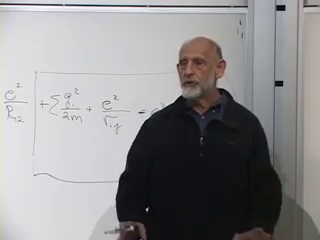
\includegraphics[width=0.72\textwidth]{lecture_01_figure_02.png}
\caption{El hamiltoniano molecular permanece en la pizarra mientras se introduce el problema del estado fundamental electrónico. La expresión mecanografiada en la ecuación~\eqref{eq:molecular-hamiltonian} recoge los términos que esta imagen no deja ver.}
\lectureframe{00:16:19}
\end{figure}

\begin{classroomqa}
\audiencequestion{¿Se están fijando sin más a cero los momentos nucleares?\lecturetimestamp{00:15:39}}
\lecturerresponse{Solo temporalmente. En la aproximación principal, los núcleos se tratan como si estuvieran clavados, porque se mueven mucho más despacio que los electrones. Recuperaremos sus momentos al resolver el problema nuclear efectivo, así que esta aproximación no viola el principio de incertidumbre.}
\end{classroomqa}

La energía del estado fundamental electrónico contribuye ahora al potencial que sienten los núcleos:
\begin{equation}
V_{\mathrm{eff}}(R_1,R_2)
=\frac{e^2}{R_{12}}+E_{\mathrm{el}}(R_1,R_2).
\label{eq:molecular-effective-potential}
\end{equation}
La invariancia rotacional y traslacional hace que, para dos átomos aislados, dependa solo de su separación \(R_{12}\). A distancias muy cortas domina la repulsión de Coulomb entre los núcleos. A distancias muy grandes, la interacción es pequeña. Entre esos límites, la nube electrónica puede producir una región atractiva y un mínimo. La función de onda nuclear se concentra entonces cerca de ese mínimo y describe una molécula ligada.

Fijémonos en el orden de las operaciones. No supusimos una atracción empírica para descartar luego los electrones. Primero resolvimos su problema cuántico en el fondo de núcleos fijos. Solo entonces eliminamos sus coordenadas explícitas y conservamos el autovalor resultante. La física de distancias cortas sobrevive en la forma, la profundidad y la curvatura de \(V_{\mathrm{eff}}\). La posición de su mínimo determina la separación de equilibrio, su curvatura controla las pequeñas vibraciones y su forma asintótica determina si existe un estado ligado. Una sola función efectiva lleva toda esa información electrónica al problema más lento.

Así, un hamiltoniano complicado de muchos electrones se ha convertido en un hamiltoniano nuclear de dos cuerpos con un potencial nuevo. Hemos eliminado los grados de libertad rápidos, pero conservado todo su efecto a baja energía. El potencial ha sido renormalizado. Este razonamiento familiar de Born--Oppenheimer no suele presentarse con ese nombre, pero contiene exactamente la idea que necesitamos:
\begin{equation}
\begin{gathered}
\text{fast microscopic dynamics}\\
\Downarrow\\
\text{effective parameters for slow dynamics}
\end{gathered}
\end{equation}

\section{Unidades naturales y dimensión de un campo}

En teoría cuántica de campos, los modos que se eliminan pueden describirse indistintamente como modos de distancias cortas, longitudes de onda cortas, frecuencias altas o energías altas. Antes de dibujar diagramas, establezcamos la contabilidad dimensional.

La mecánica ordinaria usa unidades independientes de longitud, tiempo y masa. En física de partículas fijamos
\begin{equation}
\hbar=c=1.
\end{equation}
Entonces, energía y masa son equivalentes por \(E=mc^2\), longitud y tiempo lo son porque \(c=1\), y \(\hbar=1\) hace que el momento sea el inverso de la longitud. Solo queda una dimensión:
\begin{equation}
[M]=[E]=[p]=L^{-1},
\qquad
[x]=[t]=L.
\label{eq:natural-units}
\end{equation}

Esto no elimina las dimensiones. Elige factores de conversión de modo que el tiempo pueda expresarse como una longitud y la masa como el inverso de una longitud. Una vez especificada una unidad, todas las demás se deducen. Por eso un corte puede describirse como una distancia corta \(\delta\) o como una energía alta \(\Lambda=1/\delta\): son la misma escala expresada en dos lenguajes.

Consideremos un campo escalar real \(\phi\), con una densidad lagrangiana normalizada esquemáticamente,
\begin{equation}
\mathcal L=(\partial_\mu\phi)(\partial^\mu\phi)-V(\phi),
\qquad
S=\int d^4x\,\mathcal L.
\label{eq:scalar-action}
\end{equation}

\begin{figure}[htbp]
\centering
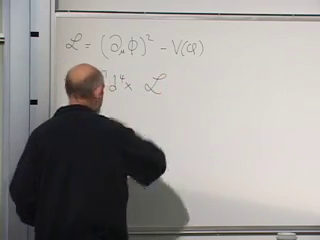
\includegraphics[width=0.78\textwidth]{lecture_01_figure_03.png}
\caption{La densidad lagrangiana escalar local y su integral sobre el espacio-tiempo, que da la acción.}
\lectureframe{00:26:08}
\end{figure}

La densidad lagrangiana es local: describe un punto del espacio-tiempo. Las ecuaciones clásicas de campo se obtienen haciendo estacionaria la acción. En teoría cuántica, la misma acción aparece en la fase de la integral de caminos \(\exp(iS)\). En cualquiera de los dos enfoques, la dimensión de \(S\) es decisiva. Al restituir \(\hbar\), la fase es \(\exp(iS/\hbar)\); una vez fijado \(\hbar=1\), \(S\) debe ser adimensional.

\begin{classroomqa}
\audiencequestion{¿La acción tiene unidades de \(\hbar\)?\lecturetimestamp{00:26:13}}
\lecturerresponse{Sí. Como se ha fijado \(\hbar\) igual a uno, en estas unidades la acción es adimensional. La medida cuatridimensional tiene dimensión \(L^4\), así que la densidad lagrangiana debe tener dimensión \(L^{-4}\).}
\end{classroomqa}

El término cinético fija ahora la dimensión del campo:
\begin{align}
[S]&=1, & [\mathcal L]&=L^{-4},\\
[\partial_\mu]&=L^{-1}, &
[(\partial\phi)^2]&=L^{-2}[\phi]^2=L^{-4},\nonumber\\
&& [\phi]&=L^{-1}.
\label{eq:scalar-dimension}
\end{align}
Este breve cálculo determinará el comportamiento ultravioleta de todos los diagramas que siguen.

Desarrollemos el potencial como
\begin{equation}
V(\phi)=\frac{m^2}{2}\phi^2+g\phi^3+\lambda\phi^4+\cdots.
\label{eq:scalar-potential}
\end{equation}
Todos los términos deben tener dimensión \(L^{-4}\). Como
\([\phi^n]=L^{-n}\),
\begin{equation}
[m^2]=L^{-2},
\qquad
[g]=L^{-1},
\qquad
[\lambda]=1.
\label{eq:coupling-dimensions}
\end{equation}
El acoplamiento cuártico es adimensional. Estos acoplamientos son especialmente importantes en la renormalización porque su dependencia de la escala no se deduce de una simple potencia de la longitud.

\begin{classroomqa}
\audiencequestion{¿\(g\) tiene unidades de masa?\lecturetimestamp{00:29:52}}
\lecturerresponse{Sí. El factor \(\phi^3\) tiene dimensión \(L^{-3}\), mientras que la densidad del potencial debe tener dimensión \(L^{-4}\). Por tanto, \([g]=L^{-1}\), que en unidades naturales es una masa.}
\end{classroomqa}

\section{Vértices y propagador a distancias cortas}

Las reglas de Feynman se construyen a partir de vértices y propagadores. El término \(g\phi^3\) da un vértice de tres líneas con un factor proporcional a \(g\); \(\lambda\phi^4\) da un vértice de cuatro líneas con un factor proporcional a \(\lambda\). El término cuadrático da una inserción local de dos puntos. Puede representarse como una partícula que entra, es absorbida y vuelve a emitirse, con un coeficiente proporcional a \(m^2/2\). Se omiten deliberadamente las normalizaciones numéricas, los signos, los factores de \(i\) y los factores de simetría, porque la clase busca extraer la dependencia de escala, no calcular una sección eficaz.

Estos dibujos tienen una interpretación operativa. Un vértice de tres puntos puede absorber dos cuantos y emitir uno, o representar cualquier asignación de sus tres líneas relacionada por cruce. Un vértice de cuatro puntos puede describir dos partículas que entran y dos que salen. La cruz cuadrática sigue siendo un vértice legítimo de dos líneas, aunque normalmente se incorpore al propagador libre. La mostramos porque pronto identificaremos todo proceso de dos puntos no resuelto comparándolo con ella.

Un propagador conecta dos puntos del espacio-tiempo. Su línea no afirma que una partícula cuántica haya seguido una trayectoria clásica rectilínea. Representa la amplitud de crear una excitación del campo en \(x\) y eliminarla o detectarla en \(y\):
\begin{equation}
\Delta(x-y)=\langle0|\phi(y)\phi(x)|0\rangle.
\label{eq:position-propagator}
\end{equation}
Leamos la expresión de derecha a izquierda. Al actuar sobre el vacío, \(\phi(x)\) crea una componente de una partícula en \(x\). Al actuar sobre el bra, \(\phi(y)\) elimina la componente en \(y\). Su elemento de matriz entre estados de vacío es la amplitud de solapamiento entre la creación en el primer punto y la detección en el segundo. Los símbolos \(x\) y \(y\) representan cuatro-vectores completos, no solo dos coordenadas cartesianas.

Los estados no tienen dimensión física, mientras que cada campo aporta \(L^{-1}\). Por tanto,
\begin{equation}
[\Delta]=L^{-2}.
\end{equation}
Para un campo sin masa no hay una escala intrínseca de longitud, así que el análisis dimensional impone el comportamiento a distancias cortas
\begin{equation}
\Delta(x-y)\sim\frac{1}{(x-y)^2}.
\label{eq:massless-propagator}
\end{equation}
El denominador es la separación al cuadrado invariante de Lorentz, con la prescripción usual necesaria en sus singularidades.\editorialnote{Para el conteo de potencias resulta conveniente hacer una rotación de Wick a una separación euclídea, donde el módulo es inequívocamente proporcional a \(1/|x-y|^2\). Esto no cambia las potencias ultravioletas que usaremos a continuación.}

Cuando \(y\) se aproxima a \(x\), el propagador diverge. Esta singularidad de la propagación a través de una separación que se anula es el origen de las divergencias ultravioletas que aparecen en diagramas más elaborados.

\section{Cómo se renormaliza la masa de un escalar}

Para un campo escalar, el parámetro dinámico es \(m^2\), como ya sugiere la relación de dispersión relativista:
\begin{equation}
E=\sqrt{\mathbf p^2+m^2}.
\end{equation}
Sea \(\delta\) la distancia más corta que resuelve nuestra descripción efectiva. No distinguiremos los procesos cuyos vértices estén separados por menos de \(\delta\). Cualquier proceso no resuelto de ese tipo, con un escalar entrante y otro saliente, tiene la misma forma observable de dos puntos que una inserción de masa y, por tanto, debe contribuir a la masa efectiva.

Pensemos en un acelerador como en un microscopio. Si su resolución más fina es \(\delta\), una absorción en un punto seguida de una emisión a una distancia mucho menor que \(\delta\) no puede distinguirse de un suceso verdaderamente local. Difuminamos deliberadamente el vértice a esa escala. La renormalización es la regla que incorpora todas esas alternativas por debajo de la resolución al coeficiente del operador local correspondiente.

\subsection{Primera corrección cuártica}

Empecemos con un único vértice \(\phi^4\). Dos líneas corresponden a la partícula externa; las otras dos se unen para formar un bucle corto que se emite y se reabsorbe casi en el mismo punto. Al promediar el propagador coincidente en la distancia de corte, obtenemos
\begin{equation}
\Delta(0)\ \longrightarrow\ \Delta(\delta)\sim\frac{1}{\delta^2},
\end{equation}
y, por tanto,
\begin{equation}
\delta m^2_{(1)}\sim\frac{\lambda}{\delta^2}.
\label{eq:one-loop-scalar-mass}
\end{equation}
Si \(m_0^2\) denota el parámetro de entrada o desnudo, el coeficiente de dos puntos a baja resolución tiene la forma esquemática
\begin{equation}
\frac{m_{\mathrm{eff}}^2}{2}
\sim
\frac{m_0^2}{2}
+c_1\frac{\lambda}{\delta^2},
\label{eq:first-renormalized-mass}
\end{equation}
donde \(c_1\) recoge los factores numéricos y dependientes de la convención que se han omitido. La masa de laboratorio medida en experimentos que no resuelven distancias menores que \(\delta\) es esta cantidad renormalizada, no \(m_0\) por sí sola.

Hay, por tanto, dos maneras indistinguibles de que ocurra el suceso observado de dos puntos. El vértice cuadrático original puede absorber y reemitir la partícula, o la interacción cuártica puede hacerlo tras emitir y reabsorber brevemente un escalar virtual. La mecánica cuántica suma las amplitudes. Cuando el bucle queda por debajo de la escala de resolución, su historia por separado desaparece de la descripción efectiva, pero su contribución al coeficiente medido permanece.

\subsection{Siguiente corrección cuártica}

Conectemos ahora dos vértices cuárticos de modo que una partícula externa entre en \(x\), otra salga de \(x+\Delta\) y tres propagadores internos unan los vértices. Hay dos potencias de \(\lambda\), mientras que los propagadores aportan \(\Delta^{-6}\). Las amplitudes cuánticas deben sumarse sobre todos los puntos no resueltos de los que puede emerger la partícula saliente, así que se integra el cuatro-vector relativo:
\begin{equation}
\delta m^2_{(2)}
\sim
\lambda^2
\int_{|\Delta|\gtrsim\delta}
d^4\Delta\,\frac{1}{|\Delta|^6}.
\label{eq:two-loop-power-count}
\end{equation}

\begin{classroomqa}
\audiencequestion{¿La pequeña marca en el vértice significa que allí solo hay tres partículas?\lecturetimestamp{00:46:35}}
\lecturerresponse{No. Seguimos usando la interacción cuártica. En cada vértice se encuentran cuatro líneas; en este diagrama de dos puntos, una es externa y tres van de un vértice al otro. El segundo vértice también tiene cuatro líneas incidentes.}
\end{classroomqa}

La medida aporta cuatro potencias de longitud y los tres propagadores, menos seis. Como el corte ultravioleta es la única escala de la estimación,
\begin{equation}
\int_{|\Delta|\gtrsim\delta}
\frac{d^4\Delta}{|\Delta|^6}
\sim\frac{1}{\delta^2},
\qquad
\delta m^2_{(2)}
\sim\frac{\lambda^2}{\delta^2}.
\label{eq:two-loop-scalar-mass}
\end{equation}
Aquí \(\Delta^\mu\) es una variable de integración de cuatro componentes; se integra sobre su componente temporal y sus tres componentes espaciales. La \(\delta\) minúscula es el corte fijo. Al principio, en la exposición oral se usa el mismo nombre para ambas y más adelante se corrige la notación.

El mismo resultado se ve al expresar radialmente la medida cuatridimensional. Salvo una constante angular,
\begin{equation}
\int_{\delta}\frac{d^4\Delta}{|\Delta|^6}
\sim
\int_{\delta}\frac{R^3\,dR}{R^6}
=\int_{\delta}\frac{dR}{R^3}
\sim\frac{1}{\delta^2}.
\end{equation}
Por eso el límite superior de distancias grandes no importa para la estimación ultravioleta: la integral está dominada por su extremo inferior.

Los diagramas de orden superior repiten el patrón. Un diagrama con más vértices cuárticos añade una potencia mayor de \(\lambda\), pero el análisis dimensional sigue permitiendo una contribución cuadráticamente divergente a la masa:
\begin{equation}
\begin{aligned}
m_{\mathrm{eff}}^2
={}&m_0^2
+\frac{1}{\delta^2}
\left(c_1\lambda+c_2\lambda^2+c_3\lambda^3+\cdots\right)\\
&+\text{weaker terms}.
\end{aligned}
\label{eq:scalar-mass-series}
\end{equation}

\subsection{La interacción cúbica y un logaritmo}

Dos vértices cúbicos contienen dos propagadores entre puntos cercanos. Su contribución escala como
\begin{equation}
\delta m_g^2
\sim
g^2\int_{|\Delta|\gtrsim\delta}
\frac{d^4\Delta}{|\Delta|^4}.
\label{eq:cubic-loop}
\end{equation}
Ahora, la medida y el denominador llevan las mismas potencias. La dependencia restante es logarítmica, en lugar de ser una potencia:
\begin{equation}
\delta m_g^2
\sim
c_g g^2\log\!\left(\frac{1}{\mu\delta}\right).
\label{eq:cubic-log}
\end{equation}
La escala de referencia \(\mu\) hace que el logaritmo sea adimensional. Esta es la versión con dimensiones correctas de la expresión esquemática de la clase \(g^2\log\delta\). Un logaritmo varía mucho más lentamente que cualquier potencia inversa, así que \(1/\delta^2\) domina cuando el corte corresponde a distancias cortas.

De nuevo, la forma radial hace patente la diferencia:
\begin{equation}
\int_{\delta}^{R_{\mathrm{IR}}}
\frac{d^4\Delta}{|\Delta|^4}
\sim
\int_{\delta}^{R_{\mathrm{IR}}}\frac{R^3\,dR}{R^4}
=\log\!\left(\frac{R_{\mathrm{IR}}}{\delta}\right).
\end{equation}
La igualdad de potencias en la medida y el denominador produce un logaritmo. Si el denominador tiene más potencias, se obtiene una potencia inversa del corte. La clase no nos pide evaluar los factores angulares; nos enseña a reconocer a simple vista la respuesta ultravioleta.

\begin{classroomqa}
\audiencequestion{¿Cuál es la base del logaritmo?\lecturetimestamp{00:57:42}}
\lecturerresponse{Se usa el logaritmo natural. Cambiar la base solo lo multiplica por una constante numérica, que queda absorbida en el coeficiente cuyos factores de \(2\), \(\pi\) y simetría no se han calculado aquí.}
\end{classroomqa}

\begin{classroomqa}
\audiencequestion{¿Cómo se puede tomar el logaritmo de una longitud y de dónde salen las unidades de la corrección de masa?\lecturetimestamp{00:58:32}}
\lecturerresponse{Un logaritmo siempre compara dos escalas; rigurosamente, es el logaritmo de una razón adimensional, como \(1/(\mu\delta)\). El acoplamiento \(g\) tiene una potencia de masa, así que \(g^2\) ya tiene exactamente la dimensión de masa al cuadrado que requiere la corrección.}
\end{classroomqa}

\begin{classroomqa}
\audiencequestion{Un diagrama de Feynman da una amplitud. ¿Su módulo al cuadrado es una probabilidad?\lecturetimestamp{00:59:41}}
\lecturerresponse{Sí, cuando la amplitud se incluye en un cálculo de una transición física con los factores de estado y de espacio de fases necesarios. Aquí su función más inmediata es distinta: una amplitud de dos puntos no resuelta tiene la misma forma local que el término de masa y, por tanto, modifica el parámetro de masa efectivo.}
\end{classroomqa}

\section{Todos los parámetros se vuelven efectivos}

La familia infinita de diagramas de masa no desaparece simplemente porque \(\lambda\) sea pequeño. La teoría de perturbaciones los ordena por potencias del acoplamiento, de modo que los términos sucesivos pueden ser menores, pero siguen siendo infinitos. La misma eliminación de procesos a distancias cortas también renormaliza las propias interacciones.

\begin{classroomqa}
\audiencequestion{¿No hay también infinitos diagramas incluso para la renormalización de la masa?\lecturetimestamp{01:00:35}}
\lecturerresponse{Sí. Si \(\lambda\) es lo bastante pequeño, la serie perturbativa puede ser útil porque las potencias sucesivas quedan cada vez más suprimidas. Sin embargo, el parámetro renormalizado se define mediante la serie completa, no solo por el primer dibujo.}
\end{classroomqa}

Desde el punto de vista operativo, una interacción local \(\lambda\phi^4\) es una amplitud con dos partículas entrantes y dos salientes. Si un proceso de cuatro puntos más complicado ocurre por entero en una región no resuelta, a baja resolución no se distingue del vértice local original. Por ello, esos diagramas se agrupan en un \(\lambda\) efectivo. En una teoría \(\phi^4\) cuatridimensional, su dependencia principal de la escala suele ser logarítmica. La clase no calcula esa función beta; usa el ejemplo para enunciar la idea general:
\begin{equation}
\begin{gathered}
\text{parameters measured at low energy}\\
\ne\\
\text{parameters entered at the microscopic cutoff}
\end{gathered}
\end{equation}

El ejemplo de cuatro puntos importa porque disipa un posible malentendido. La renormalización no es un arreglo especial que se aplica solo a la divergencia de masa. Todo operador permitido en la lagrangiana puede reproducirse mediante diagramas no resueltos con las mismas líneas externas y simetrías. Un proceso de dos puntos renormaliza un coeficiente cuadrático, uno de cuatro puntos renormaliza un coeficiente cuártico y los procesos de vacío a vacío renormalizan el término constante. La lagrangiana de baja energía es el registro compacto donde quedan asentados todos esos procesos a distancias cortas.

\begin{classroomqa}
\audiencequestion{Como \(\Delta\) tiene unidades de longitud, ¿no resulta dimensionalmente extraño tomar su logaritmo? ¿Y se intercambiaron en la pizarra las deltas mayúscula y minúscula?\lecturetimestamp{01:01:34}}
\lecturerresponse{El logaritmo se refiere en realidad a una razón respecto de otra escala y, por tanto, es adimensional. Sí, la notación se intercambió brevemente: \(\Delta^\mu\) es la variable de integración, mientras que \(\delta\) es el corte inferior de distancia que permanece en el resultado.}
\end{classroomqa}

Este es el equivalente en teoría de campos de la molécula. Resolvimos el problema de los electrones rápidos que no observamos e incorporamos el resultado a un potencial. Aquí sumamos los procesos a distancias cortas que no observamos e incorporamos el resultado a las masas, los acoplamientos y todos los demás coeficientes locales permitidos. Todo se modifica.

\begin{classroomqa}
\audiencequestion{¿Podría repetir si la cantidad medida incluye las escalas menores que las que el experimento puede detectar?\lecturetimestamp{01:05:13}}
\lecturerresponse{Sí. Sus fluctuaciones individuales no se resuelven, pero su efecto acumulado está presente. Todos los diagramas que involucran escalas más cortas se agrupan en el único coeficiente efectivo al que un experimento de baja energía llama, por ejemplo, masa física al cuadrado.}
\end{classroomqa}

\begin{classroomqa}
\audiencequestion{¿Debe entonces el término de entrada \(m_0^2\) cancelar las demás contribuciones?\lecturetimestamp{01:06:00}}
\lecturerresponse{Si la masa escalar medida es mucho menor que las contribuciones ultravioletas individuales, sí. La cancelación necesaria es el problema del ajuste fino que abordaremos ahora.}
\end{classroomqa}

\section{El problema de jerarquía del Higgs}

Imaginemos que el corte es la longitud de Planck, de modo que se pide a la teoría efectiva de campos que resuma las fluctuaciones desde las escalas de laboratorio hasta la escala en que debe intervenir la gravedad cuántica.
En unidades de física de partículas,
\begin{equation}
\delta\sim M_{\mathrm{Pl}}^{-1}\sim10^{-19}\,\mathrm{GeV}^{-1},
\qquad
\frac{1}{\delta^2}\sim10^{38}\,\mathrm{GeV}^2.
\label{eq:planck-cutoff}
\end{equation}
Para esta enorme comparación, no importa si se usa la escala de Planck reducida o la no reducida.

La jerarquía de distancias resulta igualmente sorprendente. La longitud de Planck es unos diecinueve órdenes de magnitud menor que el radio del protón y aproximadamente dieciséis o diecisiete órdenes de magnitud menor que las distancias exploradas directamente por los aceleradores mencionados. Al elevar esa separación al cuadrado se obtiene la cancelación de unas treinta y cuatro cifras en un parámetro escalar de masa al cuadrado.

Para el campo de Higgs, que es un escalar, la escala electrodébil deseada es del orden de unos cientos de GeV, no de \(10^{19}\) GeV. Sin embargo, los términos de la ecuación~\eqref{eq:scalar-mass-series} pueden tener de manera natural el orden de magnitud de la escala de Planck.
No se han determinado sus signos: algunos pueden ser positivos y otros negativos, y la masa desnuda al cuadrado también puede tener cualquiera de los dos signos. Pero, para que quede un residuo de escala electrodébil, esas contribuciones enormes deben cancelarse hasta unas treinta y cuatro cifras decimales. Susskind primero dice diecisiete cifras y luego se corrige, porque la comparación es entre masas al cuadrado. En esta versión del ajuste, lo que mide la magnitud del ajuste es la razón al cuadrado.

\begin{classroomqa}
\audiencequestion{¿Es \(\lambda\) menor o mayor que uno?\lecturetimestamp{01:09:50}}
\lecturerresponse{Se supone que es algo menor que uno. La teoría de perturbaciones se volvería intratable si las potencias sucesivas crecieran, y tampoco se puede extrapolar de manera consistente una teoría puramente escalar con un acoplamiento cuártico arbitrariamente grande. Pero \(\lambda\) no es ni de lejos tan pequeña como \(10^{-38}\); para orientarse, la conferencia toma un valor del orden de un porcentaje.}
\end{classroomqa}

\begin{classroomqa}
\audiencequestion{Aunque \(\lambda<1\), ¿no siguen siendo importantes muchos términos porque cada uno lleva el gran factor de corte?\lecturetimestamp{01:10:43}}
\lecturerresponse{Sí. Las potencias superiores acaban suprimiendo la serie, pero antes de que eso ocurra puede contribuir un gran número de términos. Todos ellos, junto con el término desnudo, tendrían que conspirar para dejar como resultado el valor físico extraordinariamente pequeño.}
\end{classroomqa}

Recordemos por qué se sabe que el parámetro de masa del Higgs está en la escala débil. En la convención de la conferencia, escribamos el potencial de ruptura de simetría como
\begin{equation}
V(\phi)=-\frac{\mu^2}{2}\phi^2+\frac{\lambda}{4}\phi^4.
\label{eq:higgs-potential}
\end{equation}
El coeficiente cuadrático negativo hace que el origen sea inestable, mientras que el término cuártico positivo estabiliza el potencial. Al derivar,
\begin{equation}
\frac{dV}{d\phi}=-\mu^2\phi+\lambda\phi^3
=\phi(-\mu^2+\lambda\phi^2),
\end{equation}
se obtiene el mínimo no nulo
\begin{equation}
\phi_{\min}^2=f^2=\frac{\mu^2}{\lambda}.
\label{eq:higgs-minimum}
\end{equation}
En la pizarra se escribe el término cuártico de forma esquemática como \(\lambda\phi^4\), pero se cita la ec.~\eqref{eq:higgs-minimum}; al incluir el factor convencional \(1/4\), ambas expresiones son coherentes sin que cambie el argumento.

El signo de \(-\mu^2\) es importante, pero no resuelve el problema de naturalidad. Lo que provoca la ruptura espontánea de simetría es la curvatura negativa en el origen. La renormalización desplaza esa curvatura mediante contribuciones grandes, tanto positivas como negativas. El vacío roto observado exige que su suma no solo sea pequeña, sino que tenga el valor negativo pequeño preciso que sitúa el mínimo en la escala débil.

Las masas de los bosones \(W\) y \(Z\) determinan que \(f\) sea del orden de \(200\,\mathrm{GeV}\) en la normalización aproximada empleada en la conferencia. Si \(\lambda\) no es ni enorme ni extraordinariamente diminuta, \(\mu\) debe ser del mismo orden general. Por tanto, el coeficiente observado en la escala débil es el residuo de contribuciones que pueden ser, cada una, decenas de órdenes de magnitud mayores.

Esto se conoce como el problema del ajuste fino del Higgs, el problema de jerarquía o el problema de jerarquía gauge. La jerarquía es la enorme razón entre la escala débil ordinaria y una posible escala de unificación o de Planck. Un número pequeño, por sí solo, no tiene por qué resultar paradójico. Lo inquietante aquí es que un número pequeño se forme a partir de contribuciones grandes y aparentemente independientes, que deben cancelarse con una precisión extrema. El problema se reconoció a finales de los 1970 y principios de los 1980, y la búsqueda de un mecanismo que explique esa cancelación motiva la supersimetría y varias ideas alternativas.

La serie perturbativa infinita agudiza el enigma, en vez de eliminarlo. Un valor de \(\lambda\) del orden de un porcentaje hace pequeñas las potencias suficientemente altas, pero antes de que esa supresión prevalezca pueden aparecer muchos términos. No basta con que un lazo cancele por accidente la masa desnuda. La escala débil efectiva debe seguir siendo estable una vez incluidas las demás contribuciones de corta distancia. Una relación estructural entre los términos sería una explicación; una cancelación dígito por dígito entre términos independientes es solo un ajuste fino.

\section{Por qué la masa de un fermión se comporta mejor}

Las demás partículas del Modelo Estándar no requieren ajustes independientes del mismo tipo. Para un fermión de Dirac, el término de masa es
\begin{equation}
\mathcal L_m=-m\bar\psi\psi
=-m\left(\bar\psi_L\psi_R+\bar\psi_R\psi_L\right).
\label{eq:fermion-mass}
\end{equation}
Contiene la masa, no su cuadrado, y acopla las quiralidades izquierda y derecha. Por tanto, una inserción local de masa transforma \(L\) en \(R\), o \(R\) en \(L\).

\begin{figure}[htbp]
\centering
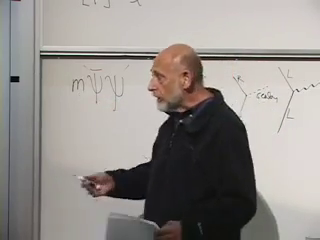
\includegraphics[width=0.76\textwidth]{lecture_01_figure_04.png}
\caption{El término de masa del fermión y los esquemas de la pizarra que muestran cambios de quiralidad. Los diagramas se reconstruyen algebraicamente a continuación, ya que parte del trabajo en la pizarra está oculta.}
\lectureframe{01:23:36}
\end{figure}

En la conferencia oral se suele hablar de lateralidad o helicidad. La protección exacta se expresa con mayor claridad en términos de quiralidad. Para una partícula ultrarrelativista, la imagen de la helicidad aporta la intuición buscada, pero la quiralidad es la propiedad que llevan los campos izquierdos y derechos en la ec.~\eqref{eq:fermion-mass}.

Las interacciones gauge conservan la quiralidad:
\begin{equation}
L\xrightarrow{\ \gamma\ }L,
\qquad
R\xrightarrow{\ \gamma\ }R.
\label{eq:gauge-preserves-chirality}
\end{equation}
Una interacción de Yukawa con un escalar conecta quiralidades opuestas:
\begin{equation}
L\xleftrightarrow{\ \phi\ }R.
\label{eq:scalar-flips-chirality}
\end{equation}
Supongamos primero que el electrón parte de \(m_0=0\). Emitir y reabsorber cualquier número de fotones no puede generar una masa, porque cada vértice gauge conserva la quiralidad. Una secuencia que empieza a la izquierda sigue siendo izquierda. Así, la electrodinámica cuántica pura permite de manera consistente un electrón sin masa: su autoenergía electromagnética no puede generar una masa aditiva a partir de cero.

En la imagen de las líneas, partamos de un electrón de quiralidad izquierda. En el primer vértice con el fotón sigue siendo de quiralidad izquierda; después de propagarse y reabsorber el fotón, también sigue siendo de quiralidad izquierda. Repetir la construcción solo añade más vértices que conservan la quiralidad. Se puede renormalizar la función de dos puntos externa, pero esta no puede adquirir la estructura izquierda-derecha que define una masa.

¿Podría lograrlo la emisión de un escalar? Un vértice escalar transforma \(L\) en \(R\), pero el escalar emitido debe reabsorberse. Por tanto, un diagrama de autoenergía de dos puntos contiene un número par de vértices escalares. El segundo cambio invierte el primero, de modo que el diagrama completo vuelve a conservar la quiralidad externa. Por complicada que se vuelva la gráfica interna, la emisión y la reabsorción emparejan los vértices e impiden que aparezca un término aditivo de \(L\) a \(R\) cuando la masa inicial es cero.

Este es un argumento de paridad sobre el número de cambios. Un vértice escalar cambia la quiralidad una vez; cerrar cada línea escalar interna requiere un segundo extremo y, por tanto, un segundo cambio. Cuatro vértices escalares producen cuatro cambios, y así sucesivamente. Un número par devuelve el fermión a su quiralidad original. La conclusión no se limita al lazo más sencillo dibujado en la pizarra.

Una corrección de masa no nula solo es posible si el diagrama ya contiene una inserción de masa. Por ejemplo, la emisión y reabsorción de un fotón pueden rodear una inserción \(m_0\bar\psi\psi\). Los vértices gauge aportan dos potencias de la carga eléctrica, pero el único cambio de quiralidad aporta la masa original:
\begin{equation}
\begin{aligned}
m_e
&=m_0+c_1e^2m_0+c_2e^4m_0+\cdots\\
&=m_0\left(1+c_1e^2+c_2e^4+\cdots\right).
\end{aligned}
\label{eq:multiplicative-fermion-mass}
\end{equation}
Si \(m_0=0\), el resultado sigue siendo cero. Si \(m_0\) es pequeña, cada corrección es proporcional a ese valor pequeño. Aún podemos preguntarnos por qué el electrón es ligero en relación con una escala fundamental, pero ya no estamos restando números enormes e independientes para obtener su masa. En este sentido, una masa fermiónica pequeña es técnicamente natural.

La inserción de masa hace explícita la secuencia permitida. Empecemos con \(L\). La emisión del fotón conserva \(L\); la inserción \(m_0\) transforma \(L\) en \(R\); la reabsorción del fotón conserva \(R\). Ahora el diagrama tiene la quiralidad externa propia de un término de masa, pero su valor contiene necesariamente el factor \(m_0\). Este es el contraste crucial con la ec.~\eqref{eq:one-loop-scalar-mass}, cuya corrección escalar sigue siendo distinta de cero incluso cuando la masa escalar inicial se fija en cero.

Los bosones gauge cuentan con una protección análoga: la simetría gauge prohíbe un término de masa independiente, por lo que un bosón gauge que parte sin masa permanece sin masa en todos los órdenes perturbativos. En el Modelo Estándar, las masas de los fermiones y de los bosones gauge débiles aparecen en respuesta al valor esperado del Higgs. Si se controla la escala del Higgs, las demás masas pequeñas no requieren copias independientes del mismo ajuste catastrófico.

Esto identifica la cuestión que la supersimetría pretende abordar: ¿puede una teoría impedir que el escalar de Higgs reciba una corrección aditiva de masa enorme? La respuesta es sí en ciertos contextos supersimétricos, porque las contribuciones bosónicas y fermiónicas están relacionadas y no son independientes. El mecanismo detallado comienza en la próxima conferencia.

\section{El otro ajuste fino: la energía del vacío}

Hay otro problema de renormalización aún más grave, pero solo se vuelve observable al incluir la gravedad. En la física no gravitatoria, sumar una constante a todas las energías no cambia ningún experimento. La masa del electrón, por ejemplo, no es una energía absoluta; es la energía adicional necesaria para añadir un electrón al vacío:
\begin{equation}
m_e=E(\text{vacuum}+\text{one electron})-E(\text{vacuum})
\end{equation}
en el sistema de reposo del electrón. Si el vacío y todos los estados excitados se desplazan juntos, sus diferencias no cambian.

Sin embargo, los diagramas de vacío a vacío sí desplazan la energía del vacío. En una teoría \(\lambda\phi^4\), se unen las cuatro patas de un vértice cuártico para formar dos lazos cortos. Cada propagador en coincidencia aporta \(1/\delta^2\), de modo que
\begin{equation}
\delta\rho_{\mathrm{vac}}
\sim
c_{\mathrm{vac}}\frac{\lambda}{\delta^4}.
\label{eq:vacuum-energy-divergence}
\end{equation}
Los diagramas de vacío más complicados llevan distintos factores de acoplamiento y coeficientes, pero el análisis dimensional suele dejar la misma sensibilidad cuártica al corte para la densidad de energía.

La ausencia de líneas externas es precisamente lo que identifica la corrección. Los diagramas de dos puntos comparan un estado de una partícula con el vacío y modifican una masa; los de cuatro puntos modifican la dispersión; un diagrama sin partículas entrantes ni salientes cambia la amplitud de vacío a vacío en sí. Un vértice cuártico aporta \(\lambda\), y sus dos lazos cortos aportan \(\delta^{-2}\) cada uno. El análisis dimensional exige entonces la escala de densidad de energía \(\delta^{-4}\).

Sin gravedad, se puede elegir el cero aditivo de la energía y preguntar a quién le importa. La relatividad general elimina esa libertad: el tensor de energía-momento es fuente de la curvatura del espacio-tiempo, así que una energía uniforme del vacío hace que el espacio vacío gravite. Aparece como una constante cosmológica y se relaciona observacionalmente con la energía oscura. Una energía del vacío medida como diminuta debe sobrevivir entonces a contribuciones de la forma \(\delta^{-4}\).

Por eso cambia la cuestión al activar la gravedad. En la mecánica cuántica ordinaria, desplazar todos los niveles en la misma constante deja intactas todas las frecuencias de transición. En gravedad, la constante no es inerte: el tensor de tensiones del vacío es proporcional a la métrica y curva el espacio-tiempo. Lo que era un cero de energía arbitrario se convierte en una fuente en la ecuación de Einstein.

Así pues, hay al menos dos problemas extremos de naturalidad. La conferencia cita aproximadamente 123 decimales de ajuste fino para la energía del vacío y aproximadamente 30--35 para la masa del Higgs. Las cifras exactas dependen de la escala ultravioleta y de las convenciones, pero el contraste es indudable. La supersimetría es una posible respuesta al problema del Higgs tratado aquí; una vez rota, no explica por sí sola la constante cosmológica observada.\editorialnote{Esta es también la razón por la que una cancelación exacta entre bosones--fermiones en una teoría supersimétrica no resuelve fenomenológicamente el problema de la energía del vacío observada: la supersimetría debe estar rota en nuestro mundo.}

\section{Preguntas finales de la clase}

\begin{classroomqa}
\audiencequestion{La corrección del Higgs depende del corte \(\delta\), pero el corte parece arbitrario. ¿Podría ser la longitud de Planck, diez veces la longitud de Planck o alguna otra cosa? ¿Eso hace que el ajuste fino sea arbitrario?\lecturetimestamp{01:33:50}}
\lecturerresponse{La contribución numérica depende de la escala más corta hasta la que se considera fiable la teoría efectiva. Esa dependencia es contabilidad física, no una vía de escape. Deben incluirse los modos hasta cualquier escala en la que el Modelo Estándar siga teniendo sentido. Elijamos \(\delta\) en la distancia donde se espera que aparezca nueva física---quizá la escala de Planck, quizá una escala de unificación cercana a \(10^{16}\,\mathrm{GeV}\). La contribución acumulada hasta esa escala ya constituye un límite inferior del problema. Extender la misma teoría a distancias aún más cortas solo aumenta la sensibilidad cuadrática. Tenemos la obligación de explicar qué cancela la contribución de cada escala entre el laboratorio y ese límite ultravioleta.}
\end{classroomqa}

\begin{classroomqa}
\audiencequestion{¿Qué define a una partícula escalar y cuál es un ejemplo?\lecturetimestamp{01:37:26}}
\lecturerresponse{El Higgs es el ejemplo que se busca. Un escalar no se transforma en componentes distintas bajo una rotación espacial; de forma equivalente, sus cuantos tienen espín cero. El fotón se describe mediante un campo vectorial y el campo gravitatorio, mediante un tensor. En el momento de esta conferencia de 2010, aún no se había detectado ninguna partícula elemental de espín cero.\editorialnote{El bosón de Higgs se descubrió en el CERN en 2012 y sus propiedades medidas son compatibles con espín cero.}}
\end{classroomqa}

\begin{classroomqa}
\audiencequestion{¿Es también la partícula \(Z\) un bosón gauge?\lecturetimestamp{01:38:31}}
\lecturerresponse{Sí. \(Z\), \(W^+\) y \(W^-\) son bosones gauge de espín uno, al igual que el fotón. Sus ecuaciones de campo y sus interacciones son generalizaciones no abelianas o electrodébiles de la descripción gauge de tipo Maxwell.}
\end{classroomqa}

\begin{classroomqa}
\audiencequestion{¿Por qué la contribución bosónica del estado fundamental no cancela la fermiónica en la energía del vacío?\lecturetimestamp{01:39:10}}
\lecturerresponse{Los lazos de fermiones y los correspondientes lazos de bosones pueden, en efecto, entrar con signos opuestos. Sin embargo, la cancelación no es automática: las masas, multiplicidades y acoplamientos de las partículas deben coincidir. Incluso una pequeña discrepancia deja un residuo grande y sensible al corte, y las infinitas familias de diagramas deben coincidir orden por orden. La supersimetría exacta impone precisamente esas relaciones entre bosones--fermiones. El contenido genérico de partículas no supersimétrico no las impone, y la supersimetría rota deja un problema residual de energía del vacío.}
\end{classroomqa}

\section{Perspectiva}

El recorrido de la conferencia sigue un orden deliberado. Primero, un cálculo molecular muestra que eliminar las variables rápidas no es ni ignorarlas ni recurrir a la magia: su energía de estado fundamental se convierte en un potencial para las variables lentas. La teoría cuántica de campos repite esa operación a través de las longitudes de onda. El análisis dimensional revela entonces qué parámetros efectivos son sensibles al corte. Las masas escalares reciben términos aditivos proporcionales a \(\delta^{-2}\); por tanto, la pequeña escala del Higgs parece delicadamente antinatural. Las masas de los fermiones se renormalizan multiplicativamente porque la quiralidad protege el límite de masa nula, y la simetría gauge protege de forma análoga a los bosones gauge sin masa. La energía del vacío es aún más sensible: escala como \(\delta^{-4}\), y la gravedad hace observable su valor absoluto.

La supersimetría aparece en el curso justo en este punto, no como matemática nueva meramente ornamental, sino como un intento de hacer que el sector escalar se comporte más como los sectores protegidos. La tarea siguiente es entender qué simetría puede relacionar bosones y fermiones con la fuerza suficiente para organizar esas cancelaciones.
\chapter{Signos fermiónicos y cancelaciones supersimétricas}

\lectureoverview{La supersimetría relaciona bosones con fermiones, pero resulta más fácil entender por qué se busca una relación así antes de escribir su álgebra. Empezaremos con la topología de las rotaciones, haremos observable mediante interferencia el signo de la función de onda de un fermión, deduciremos el signo negativo de un bucle fermiónico cerrado a partir de la antisimetría bajo intercambio y, después, usaremos los signos opuestos de los bucles bosónicos y fermiónicos para motivar las cancelaciones de la energía del vacío y de la autoenergía escalar. En la segunda mitad preguntaremos cuán fuertemente puede romperse la supersimetría, cómo podrían detectarse los supercompañeros y por qué una supersimetría exacta eliminaría la estructura ordinaria de capas atómicas.}

\section{Antes de la supersimetría: una peculiaridad de las rotaciones}

La supersimetría es una simetría entre fermiones y bosones. Sin embargo, antes de intentar construirla, conviene recordar cuán distinta es la respuesta de estos dos tipos de partículas a las rotaciones. Esta cuestión parte de un hecho topológico fácil de demostrar y sorprendentemente difícil de olvidar una vez que se ha visto.

Mantén una mano con la palma hacia arriba y gira la muñeca a través de \(2\pi\). La mano recupera su orientación original, pero es evidente que el brazo no ha vuelto a una configuración equivalente: está retorcido. Continúa otros \(2\pi\), moviendo el brazo como haga falta, y podrás deshacer la torsión. Así pues, una rotación de \(2\pi\) no puede deformarse continuamente hasta quedar en ninguna rotación mientras se mantienen fijos los alrededores, mientras que una rotación de \(4\pi\) sí. La demostración con la mano es una prueba hecha con las manos en el sentido más literal.

La misma idea puede ilustrarse sin recurrir a la anatomía. Coloca una pelota dentro de una caja fija y sujétala a las paredes con cualquier número de cuerdas flexibles, elásticas, pero irrompibles. Gira la pelota una vez, un ángulo de \(2\pi\). Las cuerdas se enredan y ningún movimiento de las cuerdas por sí solas restaura la configuración original. Gira la pelota hasta completar un ángulo total de \(4\pi\) y podrás llevar las cuerdas a su alrededor hasta que desaparezca el enredo. Las paredes representan el infinito espacial: la comparación solo tiene sentido porque el contorno no gira junto con la pelota.

\begin{classroomqa}\audiencequestion{¿Se podría deshacer el enredo girando la caja? \lecturetimestamp{00:02:53}}\lecturerresponse{Eso cambiaría el problema. La caja representa el infinito espacial y se mantiene fija. Comparamos la rotación del objeto con respecto a sus alrededores, no una rotación conjunta del objeto y sus alrededores.}\end{classroomqa}

\begin{classroomqa}\audiencequestion{¿Por qué no girar simplemente la pelota otros \(2\pi\)? \lecturetimestamp{00:03:20}}\lecturerresponse{Eso es precisamente lo que distingue los dos casos. Sin volver a girar la pelota, no se puede deshacer el enredo que deja un giro de \(2\pi\). Tras el segundo giro, que completa \(4\pi\), sí se puede.}\end{classroomqa}

En el lenguaje moderno de grupos, el grupo de rotaciones tiene dos clases topológicas de caminos cerrados:
\begin{equation}
\pi_1\!\left(SO(3)\right)\cong \mathbb Z_2.
\end{equation}
Un recorrido es no trivial, pero recorrerlo dos veces da la clase trivial.
De manera equivalente, \(SU(2)\) es el recubrimiento doble de \(SO(3)\). Esta es la prehistoria geométrica del signo fermiónico.

\editorialnote{El lenguaje de \(SO(3)\), \(SU(2)\) y el grupo fundamental hace explícita la topología. Las demostraciones del brazo y de las cuerdas establecen geométricamente el mismo comportamiento de dos valores.}

\section{Qué le hace una rotación de \texorpdfstring{\(2\pi\)}{ pi2 a un estado cuántico}}

Fijemos ahora la posición de una partícula y conservemos únicamente su estado de espín, denotado por \(\ket{\psi}\). Las partículas de espín entero son bosones y las de espín semientero son fermiones. Una rotación física puede realizarse colocando un espín cargado en un campo magnético intenso y girando el campo, o haciendo que el espín precesione el ángulo deseado en un campo fijo.

\begin{classroomqa}\audiencequestion{¿Cómo se puede girar realmente el espín de un electrón en el laboratorio? \lecturetimestamp{00:05:26}}\lecturerresponse{Un campo magnético proporciona el medio para hacerlo. Se puede girar un campo suficientemente intenso para que el espín lo siga, o dejar que el espín precesione alrededor de un campo fijo. Agarrar el electrón con la mano no es un método experimental competitivo.}\end{classroomqa}

Supongamos que una rotación completa de \(2\pi\) multiplica el estado por una fase:
\begin{equation}
R(2\pi)\ket{\psi}=\xi\ket{\psi}.
\end{equation}
Al realizar la operación dos veces, se obtiene
\begin{equation}
R(4\pi)\ket{\psi}=\xi^2\ket{\psi}.
\end{equation}
Como el camino de \(4\pi\) es topológicamente trivial, en esta comparación debe actuar como la identidad. Por tanto,
\begin{equation}
\xi^2=1,
\qquad
\xi=+1\ \hbox{or}\ -1.
\end{equation}
Los bosones realizan el signo positivo y los fermiones, el negativo:
\begin{align}
R(2\pi)\ket{\psi_B}&=+\ket{\psi_B},\\
R(2\pi)\ket{\psi_F}&=-\ket{\psi_F}.
\end{align}
Para un estado de espín definido \(j\), la expresión compacta es
\begin{equation}
R(2\pi)=(-1)^{2j}.
\end{equation}
La transcripción dice brevemente que la segunda posibilidad corresponde a una multiplicación por \(2\pi\); la derivación y el argumento de la pizarra dejan claro que el factor previsto es \(-1\).

Al principio, esto parece no tener consecuencias físicas. Si cambia el signo de toda una función de onda,
\begin{equation}
\Psi\longmapsto-\Psi,
\end{equation}
las probabilidades no cambian, porque
\begin{equation}
(-\Psi)^*(-\Psi)=\Psi^*\Psi.
\end{equation}
Tomemos dos conjuntos de electrones preparados de manera idéntica. Giremos cada electrón de uno de los conjuntos un ángulo de \(2\pi\) y dejemos intacto el otro conjunto. Ninguna medición de un electrón aislado puede revelar a cuál de los dos conjuntos pertenecía. Una fase global no es observable.

\section{Hacer relativo el signo negativo}

El signo se vuelve observable cuando se impone a una rama coherente de la función de onda, pero no a la otra. Enviemos electrones de uno en uno por un aparato de dos caminos. No determinemos qué camino sigue cada electrón, pues la información sobre el camino destruye la interferencia. Sean \(\psi_1\) y \(\psi_2\) las amplitudes de los caminos superior e inferior, de modo que el estado recombinado sea
\begin{equation}
\Psi=\psi_1+\psi_2.
\end{equation}
Imaginemos por un momento que atrapamos cada rama en una región magnética. Giremos el campo asociado a la segunda rama un ángulo de \(2\pi\). Si la partícula es un fermión, el estado pasa a ser
\begin{equation}
\Psi'=\psi_1-\psi_2.
\end{equation}
Ya no se trata de un signo global. La fase relativa desplaza los máximos de interferencia y los convierte en mínimos. Si los dos paquetes que regresan son imágenes especulares respecto del centro del detector, la combinación antisimétrica se anula en el centro:
\begin{equation}
\Psi'(0)=\psi_1(0)-\psi_2(0)=0.
\end{equation}
Por tanto, el electrón nunca se detecta en ese punto de simetría. En cambio, girar ambas ramas produciría \(-\psi_1-\psi_2=-\Psi\), lo cual no tendría ningún efecto observable.

La clase destaca el carácter relacional del experimento. Girar una región magnética con respecto a la otra es análogo a girar la pelota manteniendo fija la caja. Girar ambas regiones a la vez es análogo a girar conjuntamente la pelota y la caja. Una rotación relativa de \(4\pi\) elimina el efecto porque entonces el estado fermiónico vuelve con signo positivo. Yakir Aharonov y Leonard Susskind propusieron el experimento en 1967 y, como se señala brevemente en los apuntes de clase, más tarde se realizó en forma interferométrica. El mismo principio puede aplicarse a electrones o iones cargados: un patrón de franjas desplazado identifica un estado de espín semientero, mientras que uno sin desplazar identifica un estado de espín entero.

\begin{classroomqa}\audiencequestion{Si el campo relativo se gira \(4\pi\), ¿vuelve el patrón desplazado al original? \lecturetimestamp{00:12:21}}\lecturerresponse{Sí. Dos cambios de signo se multiplican y dan \(+1\), así que desaparece la fase relativa que intercambia los máximos y los mínimos.}\end{classroomqa}

\begin{classroomqa}\audiencequestion{¿Hasta qué punto hay que tomar literalmente las cuerdas de la caja al relacionarlas con un fermión? \lecturetimestamp{00:13:43}}\lecturerresponse{Son una imagen mnemotécnica topológica, no cuerdas físicas atadas a un electrón. Un bosón se comporta como si un giro de \(2\pi\) no dejara rastro; un fermión conserva precisamente la memoria del signo representada por el enredo no trivial.}\end{classroomqa}

\begin{classroomqa}\audiencequestion{¿Hay dos electrones en las dos regiones magnéticas, uno girado y otro sin girar? \lecturetimestamp{00:14:29}}\lecturerresponse{No. Hay un único electrón en una superposición espacial coherente. Tiene una amplitud de probabilidad de ocupar cada una de las ramas, y el aparato no debe revelar cuál ocupó. Girar una región cambia una amplitud con respecto a la otra; girar ambas cambia solo la fase común.}\end{classroomqa}

El ángulo \(2\pi\) es especial porque la orientación del espín vuelve a sí misma mientras el espinor adquiere un signo. Una rotación relativa genérica también cambia la orientación del espín. Si los estados de los dos caminos regresan con estados de espín \(\ket{\chi_1}\) y \(\ket{\chi_2}\), el término de interferencia es proporcional a
\begin{equation}
\braket{\chi_1}{\chi_2}.
\end{equation}
Su módulo determina la visibilidad de las franjas.\editorialnote{}La fórmula del solapamiento de espines completa de manera estándar el análisis cualitativo de la clase sobre la pérdida parcial y total de interferencia. Los estados de espín ortogonales llevan información perfecta sobre el camino y no interfieren.

\begin{classroomqa}\audiencequestion{¿Qué ocurre si se mide en cuál de las regiones magnéticas estaba el electrón? \lecturetimestamp{00:18:03}}\lecturerresponse{El patrón de interferencia se destruye. Cualquier registro que permita distinguir los dos caminos elimina la suma coherente de sus amplitudes.}\end{classroomqa}

\begin{classroomqa}\audiencequestion{Si todos los espines parten en la misma dirección y se mide el espín final, ¿la operación de \(2\pi\) cambia esa dirección por sí misma? \lecturetimestamp{00:18:17}}\lecturerresponse{No. Después de \(2\pi\), la dirección física del espín es la misma; solo la rama fermiónica ha adquirido un signo negativo. Por eso esta operación puede cambiar la interferencia sin dejar una orientación distinta del espín que sirva como indicador del camino.}\end{classroomqa}

\begin{classroomqa}\audiencequestion{¿Qué ocurre si el campo solo se gira un ángulo de \(\pi\) en vez de \(2\pi\)? \lecturetimestamp{00:18:43}}\lecturerresponse{Entonces cambia la dirección del espín. Una rama con espín hacia arriba y otra con espín hacia abajo pueden distinguirse y no interfieren. Los ángulos intermedios reducen gradualmente la visibilidad; un giro relativo de \(180^\circ\) la destruye por completo.}\end{classroomqa}

\section{Simetría de intercambio y signo de un bucle cerrado}

La discusión de las rotaciones ha aislado un signo negativo fermiónico. Al intercambiar partículas idénticas aparece otro signo estrechamente relacionado. Para una función de onda de dos partículas,
\begin{align}
P_{12}\Psi_B(1,2)&=+\Psi_B(1,2)=+\Psi_B(2,1),\\
P_{12}\Psi_F(1,2)&=-\Psi_F(1,2)=-\Psi_F(2,1).
\end{align}
Los estados bosónicos son simétricos y los fermiónicos, antisimétricos.

\begin{figure}[htbp]\centering
\includegraphics[width=0.74\textwidth]{lecture_02_figure_02.png}\lectureframe{00:24:27}\caption{El argumento del intercambio en notación de estados. En el fotograma solo se distingue con seguridad la etiqueta del vector de estado; las ecuaciones de antisimetría aparecen escritas en el texto y no se atribuyen a la tiza que queda oculta.}\end{figure}

Ahora podemos determinar el signo relativo de un bucle cerrado de partículas sin calcular su integral. Consideremos un diagrama de Feynman del vacío, sin líneas externas. Puede imaginarse como una partícula que recorre un camino cerrado en el espacio-tiempo, o como un par partícula-antipartícula que se crea y luego se aniquila. Un diagrama de vacío de este tipo contribuye a la amplitud del vacío y, por tanto, a la energía del vacío.

Empecemos con dos copias desconectadas del bucle. Los diagramas desconectados se multiplican, así que, si un bucle tiene signo \(\sigma\), el par tiene signo
\begin{equation}
\sigma^2=+1.
\end{equation}
Cortemos ambos bucles en un instante común, por ejemplo \(t=0\). En ese instante hay dos partículas idénticas. Si las reconectamos sin intercambiarlas, reaparecen los dos bucles separados. Si intercambiamos las partículas antes de reconectarlas, la topología se convierte en un solo bucle. El intercambio aporta \(+1\) para los bosones y \(-1\) para los fermiones. Como el signo inicial de los dos bucles era positivo, los signos resultantes para un único bucle son
\begin{equation}
\begin{aligned}
\operatorname{sign}(\text{closed boson loop})&=+1,\\
\operatorname{sign}(\text{closed fermion loop})&=-1.
\end{aligned}
\end{equation}
En general, un diagrama con \(L_F\) bucles fermiónicos cerrados independientes lleva el factor
\begin{equation}
(-1)^{L_F}.
\end{equation}
La clase deduce deliberadamente esta regla a partir del intercambio, en vez de invocar la integración de Grassmann. Este argumento elemental hace visible el origen físico del signo.

\section{Signos opuestos de los bucles y energía del vacío}

Un bucle bosónico del vacío eleva la contribución del vacío con un signo, mientras que un bucle fermiónico aporta el signo opuesto. Esto resulta sugerente de inmediato, porque la densidad de energía oscura observada es extremadamente pequeña en comparación con las estimaciones ingenuas de la teoría cuántica de campos basadas en un corte. La clase cifra la discrepancia, notoria desde hace tiempo, en aproximadamente \(123\) órdenes de magnitud. El exponente preciso depende de la escala ultravioleta que se utilice; lo que perdura es la enorme discrepancia.

El valor de un bucle depende de más que la estadística. Depende de la masa, la carga, la multiplicidad y las interacciones. Sin embargo, si un bosón y un fermión coinciden en todas las propiedades pertinentes, sus contribuciones de igual magnitud pueden cancelarse:
\begin{equation}
\begin{gathered}
m_B=m_F,\qquad q_B=q_F,\qquad g_B=g_F,\\
\Delta\rho_{\mathrm{vac}}^{(B)}
+\Delta\rho_{\mathrm{vac}}^{(F)}=0.
\end{gathered}
\end{equation}
Esta observación no resuelve el problema de la constante cosmológica. Solo aporta algo que los bucles bosónicos ordinarios por sí solos no podían aportar: contribuciones de signo opuesto. En una teoría global supersimétrica exactamente no rota, las cancelaciones de la energía del vacío pueden ser exactas bajo los supuestos adecuados; una vez rota la supersimetría, el pequeño valor no nulo observado sigue sin explicación.\editorialnote{Esta precisión distingue la motivación presentada en la clase del problema, mucho más difícil, de la constante cosmológica.}

Ya sabemos que la coincidencia exacta no describe la naturaleza. Si el electrón tuviera un supercompañero de espín cero con la misma masa y carga eléctrica, la aniquilación de un electrón y un positrón a través de un fotón virtual podría producir un par de ellos:
\begin{equation}
e^-e^+\longrightarrow\gamma^*
\longrightarrow\widetilde e^-\widetilde e^+.
\end{equation}
Un escalar cargado degenerado no habría pasado inadvertido en los experimentos ordinarios de colisionadores. Así pues, la correspondencia entre bosones y fermiones no puede ser una simetría exacta del espectro observado. Se trata de una correspondencia entre tipos de partículas, no de una reflexión en el espacio físico.

\section{El objetivo más inmediato: la autoenergía escalar}

La energía del vacío es el primer ejemplo, pero la principal preocupación de la clase es la inestabilidad radiativa de las masas escalares. Un escalar que parte de masa desnuda nula puede recibir una corrección que depende cuadráticamente del corte. Esquemáticamente,
\begin{equation}
\Delta m_H^2\sim \frac{g_B^2}{16\pi^2}\Lambda^2
\end{equation}
procede de un bucle bosónico. Las masas de los fermiones cuentan con otra protección: cuando un fermión sin masa tiene una simetría quiral exacta, las correcciones radiativas no pueden generar un término de masa aditivo. Ese fue el argumento izquierda-derecha de la clase anterior.

Imaginemos ahora una simetría lo bastante rígida como para reunir un escalar y un fermión en un mismo multiplete y hacer coincidir sus interacciones. Entonces aparece un bucle fermiónico con el signo opuesto:
\begin{equation}
\Delta m_H^2
\sim
\frac{g_B^2-g_F^2}{16\pi^2}\Lambda^2+\cdots .
\end{equation}
Si la supersimetría impone \(g_B=g_F\) e igualdad de masas, los términos cuadráticos se cancelan. Así se transmite al compañero bosónico la protección de la que goza el fermión. No se trata solo de una coincidencia numérica entre dos diagramas; la simetría debe imponer la cancelación a todos los órdenes y mediante todas las interacciones permitidas.

La comparación amplia en la pizarra muestra cómo la clase pasa de bucles aislados a correcciones de bucle emparejadas para partículas que se propagan.

\begin{figure}[htbp]
\centering
\includegraphics[width=0.79\textwidth]{lecture_02_figure_04.png}
\lectureframe{00:40:23}

\medskip
\begin{tikzpicture}[scale=0.9]
\draw (-4.2,0) circle (0.55);
\draw[dashed] (-2.4,0) circle (0.55);
\draw (0,0) -- (3.7,0);
\fill (1.85,0) circle (0.055);
\draw (1.85,0) -- (1.85,0.25);
\draw[dashed] (1.85,0.85) circle (0.6);
\end{tikzpicture}\caption{Comparación general de las topologías de bucle ordinarias y las de los supercompañeros. El esquema transcrito conserva solo el contraste topológico visible; no asigna etiquetas a partículas que quedan ocultas.}\end{figure}

Tras la pausa de la clase, el argumento se retoma con lo que se llama el cuadro de orden cero. Esto no indica un orden en la teoría de perturbaciones, sino la descripción útil más esquemática:
\begin{quote}
Toda partícula tiene un supercompañero de estadística opuesta. Cada fermión tiene un compañero bosónico y cada bosón, uno fermiónico.
\end{quote}
En una teoría supersimétrica exacta, los supercompañeros también serían degenerados, es decir, tendrían la misma masa. La naturaleza no presenta esta degeneración. Aun así, si las masas son distintas pero no demasiado, la cancelación podría seguir siendo lo bastante eficaz como para evitar una corrección escalar desmesuradamente grande. Con una ruptura suave de la supersimetría, la escala peligrosa se sustituye esquemáticamente por la separación entre las masas de los supercompañeros:
\begin{equation}
\Delta m_H^2\sim
\frac{g^2}{16\pi^2}\,\Delta m_{\mathrm{SUSY}}^2
\ln\!\frac{\Lambda^2}{\Delta m_{\mathrm{SUSY}}^2}
\end{equation}
hasta factores que dependen del modelo.\editorialnote{Esta fórmula expresa la afirmación cualitativa de la clase: una correspondencia imperfecta entre masas deja una corrección residual determinada por la separación entre ellas; no es una transcripción de la pizarra.}

\section{Supersimetría rota y la apuesta experimental de 2010}

No se había observado ningún supercompañero cuando se grabó esta clase en 2010. La inferencia inmediata era que, si los supercompañeros existían, tenían que ser más pesados que las partículas conocidas y estar fuera del alcance de los aceleradores anteriores. Los modelos supersimétricos también distinguen las partículas cuyas masas solo aparecen tras la ruptura de la simetría electrodébil de los estados que pueden tener masas mayores sin romper la simetría. La clase propone esto como justificación de que la mitad visible de un espectro supersimétrico pudiera ser ligera, mientras que la mitad no observada fuera más pesada, y reconoce francamente que esta propuesta exige cierto esfuerzo de aceptación. Susskind expresa su propia expectativa de que se detectarían supercompañeros e inmediatamente aclara que es una conjetura, no un resultado.

Por tanto, el Gran Colisionador de Hadrones ocupaba un lugar central en las perspectivas que planteaba la conferencia. Se esperaba que buscara tanto el bosón de Higgs como las superpartículas. Estas afirmaciones deben leerse en su contexto de 2010: la conferencia explica la apuesta experimental antes del descubrimiento del Higgs y de los resultados posteriores de las búsquedas en el LHC.

¿Por qué un supercompañero motivado por la naturalidad no debería encontrarse a la escala de Planck? Porque en tal caso no cumpliría la función que se le asigna. Si las masas de los bosones y los fermiones difieren enormemente, las integrales de bucle dejan de cancelarse por encima de la masa menor. La corrección escalar residual queda determinada, aproximadamente, por la gran separación entre las masas y no por la escala electrodébil. La supersimetría a una escala arbitrariamente remota sigue siendo una simetría matemática, pero ya no ofrece una explicación convincente de por qué el sector de Higgs es ligero.

La clase traduce esta idea en la expectativa propia de su época de que las separaciones pertinentes entre masas debían ser del orden de unos pocos cientos de GeV y, por tanto, estar al alcance del LHC. Esta estimación numérica es histórica y depende del modelo; la cadena lógica es más importante:
\begin{equation}
\begin{gathered}
\text{Higgs protection}\\
\Downarrow\\
\text{effective boson--fermion cancellation}\\
\Downarrow\\
\Delta m_{\mathrm{SUSY}}\ \text{not too large}.
\end{gathered}
\end{equation}

\begin{classroomqa}\audiencequestion{¿Podrían cancelarse simplemente en conjunto todas las contribuciones fermiónicas con todas las contribuciones bosónicas, sin supercompañeros uno a uno? \lecturetimestamp{00:45:01}}\lecturerresponse{Podrían cancelarse numéricamente, pero sería una cancelación accidental tan finamente ajustada como el problema original. La propuesta supersimétrica es más fuerte: unos postulados razonables imponen contribuciones correspondientes, mientras que la ruptura de la supersimetría explica por qué las masas solo coinciden de manera aproximada. La energía del vacío sirvió de ejemplo; la preocupación inmediata aquí es la autoenergía del Higgs.}\end{classroomqa}

\begin{classroomqa}\audiencequestion{¿Llamar antinatural a una cancelación global presupone ya una forma reduccionista de organizar la teoría? \lecturetimestamp{00:47:51}}\lecturerresponse{Es una objeción legítima. Nadie tiene una definición definitiva de naturalidad, y la búsqueda consiste en parte en tantear en busca de una explicación convincente. La supersimetría y la ruptura espontánea de la supersimetría ofrecen marcos matemáticos conocidos que pueden imponer el patrón deseado. Queda por resolver si la naturaleza utiliza ese marco y si es único.}\end{classroomqa}

\section{Producción directa, efectos virtuales y cadenas de desintegración}

No es necesario producir una partícula pesada en su capa de masa para que influya en un experimento. Puede aparecer virtualmente dentro de un lazo y modificar ligeramente una amplitud ordinaria de dispersión electrón-positrón. Por tanto, las mediciones de precisión electrodébil imponen restricciones a las superpartículas incluso cuando la energía del centro de masas está por debajo del umbral de producción directa de pares
\begin{equation}
\sqrt{s}<2m_{\widetilde p}.
\end{equation}
La evaluación de 2010 en la conferencia es que los datos de precisión ya estaban acotando el espacio de parámetros supersimétricos, pero aún no lo habían descartado.

\begin{classroomqa}\audiencequestion{¿Se podrían inferir indirectamente los supercompañeros, como se restringieron las propiedades de partículas pesadas anteriores mediante tasas de producción precisas antes de observarlas directamente? \lecturetimestamp{00:49:01}}\lecturerresponse{Sí. Un bucle virtual de supercompañero altera ligeramente una amplitud ordinaria, así que el problema pasa a ser la fenomenología electrodébil de alta precisión, en vez de la producción directa. Sería especialmente útil un colisionador electrón-positrón limpio y con energía suficiente. Las colisiones de protones son más confusas porque el protón es un estado compuesto de quarks y gluones: en realidad colisionan sus constituyentes fluctuantes, no dos partículas elementales cuyas condiciones iniciales se conozcan con precisión.}\end{classroomqa}

Un estudiante pregunta por la reacción inversa, partiendo de abundantes superpartículas. El obstáculo no es la simetría de inversión temporal, sino la disponibilidad. Primero hay que crear los supercompañeros pesados, y se espera que la mayoría se desintegre rápidamente en estados más ligeros.

\begin{classroomqa}\audiencequestion{Si un universo contuviera muchas superpartículas, ¿podrían dos de ellas colisionar y transformarse en partículas ordinarias? \lecturetimestamp{00:53:43}}\lecturerresponse{En principio, las reacciones pertinentes tienen canales inversos, pero no se espera que los supercompañeros pesados sigan presentes en abundancia como partículas libres. Se desintegran hacia estados de menor energía, así que un experimento debe aportar primero suficiente energía de colisión para crearlos.}\end{classroomqa}

Esto plantea la cuestión de la materia oscura. En muchos modelos supersimétricos, una regla de selección discreta impide que desaparezca por completo el último supercompañero de una cadena de desintegración. En tal caso, todos los supercompañeros más pesados van desintegrándose hasta llegar al supercompañero más ligero, o LSP. Si el LSP es eléctricamente neutro, puede ser estable y difícil de detectar, lo que lo convierte en un posible candidato a materia oscura. En este intercambio, la transcripción dice una vez «energía oscura», pero la pregunta del público y la descripción de la partícula se refieren inequívocamente a la materia oscura.

\begin{classroomqa}\audiencequestion{¿Es incompatible la rápida desintegración de los supercompañeros con la propuesta de que uno de ellos podría constituir materia oscura? \lecturetimestamp{00:54:53}}\lecturerresponse{No. En los modelos que requieren un supercompañero al final de cada cadena de desintegración, la mayoría de los supercompañeros puede desintegrarse mientras el más ligero permanece estable. La carga eléctrica suele plantear dificultades fenomenológicas adicionales, así que es probable que el LSP viable sea neutro. No es indetectable en principio, pero no dejaría la señal evidente de ionización que dejaría un selectrón cargado.}\end{classroomqa}

\section{La correspondencia exige que coincidan los acoplamientos}

La correspondencia entre masas por sí sola no basta. Comparemos un bucle del vacío de un electrón con uno de un selectrón. Sus estadísticas opuestas aportan signos opuestos, pero para que las magnitudes sean iguales hace falta que las masas coincidan. Si ahora añadimos dos fotones externos, los coeficientes también contienen los acoplamientos eléctricos, así que la cancelación requiere que las cargas sean iguales:
\begin{equation}
\begin{gathered}
q_{\widetilde e}=q_e,\\
\mathcal A_{\mathrm{loop}}^{(e)}
+\mathcal A_{\mathrm{loop}}^{(\widetilde e)}=0,\\
\text{provided the full couplings match.}
\end{gathered}
\end{equation}
Una discrepancia en cualquier aspecto deja un término divergente sin cancelar. La supersimetría es valiosa porque relaciona las interacciones, además de los nombres y los espines.

\begin{figure}[H]
\centering
\includegraphics[width=0.66\textwidth]{lecture_02_figure_05.png}
\lectureframe{00:57:15}

\medskip
\begin{tikzpicture}[scale=0.9]
\draw (-2.0,0) circle (0.85);
\draw[dashed] (2.0,0) circle (0.85);
\node at (-2.0,-1.2) {fermion loop};
\node at (2.0,-1.2) {bosonic partner loop};
\end{tikzpicture}\caption{Comparación de bucles continuos y discontinuos durante el argumento de la correspondencia de cargas. No se reconstruyen las marcas externas recortadas, porque el fotograma por sí solo no permite determinar todos los puntos de inserción.}\end{figure}

\begin{classroomqa}\audiencequestion{¿Podrían haber pasado inadvertidos los supercompañeros sencillamente porque sus constantes de acoplamiento son distintas? \lecturetimestamp{00:56:23}}\lecturerresponse{No, si se pretende que los mismos diagramas se cancelen. Añadir interacciones con fotones permite comprobar la carga eléctrica de cada línea. Unos acoplamientos desiguales producen factores de bucle numéricos distintos y restablecen el gran residuo. La simetría debe hacer coincidir las cargas e interacciones pertinentes.}\end{classroomqa}

\begin{classroomqa}\audiencequestion{¿También debería ser sin masa el supercompañero del fotón? \lecturetimestamp{00:58:01}}\lecturerresponse{Sería sin masa en una teoría supersimétrica exacta, pues tendría la misma masa que el fotón. El mundo observado no es exactamente supersimétrico, así que un estado físico similar al fotino no tiene por qué compartir la masa del fotón.}\end{classroomqa}

\section{El diccionario de los supercompañeros}

Las reglas para formar los nombres no son elegantes, pero sí útiles. A un bosón se le asigna un compañero fermiónico cuyo nombre suele terminar en \emph{-ino}: fotón y fotino, \(W\) y wino, \(Z\) y zino, gluón y gluino, Higgs e higgsino, gravitón y gravitino. A un fermión ordinario se le asigna un compañero bosónico cuyo nombre suele empezar por \emph{s-}: electrón y selectrón, quark y squark.

\begin{center}
\begin{tabular}{@{}>{\raggedright\arraybackslash}p{0.40\linewidth}>{\raggedright\arraybackslash}p{0.52\linewidth}@{}}
\toprule
estado ordinario & supercompañero y cambio de espín\\
\midrule
Higgs escalar, \(j=0\) & higgsino, \(j=\tfrac12\); \(\Delta j=+\tfrac12\)\\
bosón gauge, \(j=1\) & gaugino, \(j=\tfrac12\); \(\Delta j=-\tfrac12\)\\
fermión de materia, \(j=\tfrac12\) & sfermión, \(j=0\); \(\Delta j=-\tfrac12\)\\
gravitón, \(j=2\) & gravitino, \(j=\tfrac32\); \(\Delta j=-\tfrac12\)\\
\bottomrule
\end{tabular}
\end{center}

La relación general es que los miembros de un supermultiplete difieren en media unidad de espín:
\begin{equation}
\Delta j=\frac12.
\end{equation}
Los ejemplos esquemáticos de la clase emparejan un fermión de materia de espín \(\tfrac12\) con un escalar, y un bosón gauge de espín uno con un gaugino de espín \(\tfrac12\). En un modelo completo con interacciones, los estados pueden mezclarse tras la ruptura de simetría, por lo que los autoestados físicos de masa quizá no conserven estos nombres más sencillos.

\begin{classroomqa}
\audiencequestion{¿Podrían todos los nuevos compañeros escalares experimentar su propia ruptura espontánea de simetría? \lecturetimestamp{01:01:27}}
\lecturerresponse{Los campos escalares pueden adquirir valores esperados, pero una ruptura de simetría adicional arbitraria tendría consecuencias fenomenológicas desastrosas. Un modelo supersimétrico viable debe organizar su potencial escalar de modo que el color, la carga eléctrica y las demás simetrías necesarias no se rompan de forma inadecuada.}
\end{classroomqa}

\begin{classroomqa}
\audiencequestion{¿Tiene el higgsino interacciones especiales correspondientes al término cuártico del Higgs? \lecturetimestamp{01:02:19}}
\lecturerresponse{La supersimetría relaciona tanto las interacciones como las partículas. La relación no se obtiene sustituyendo ingenuamente cada línea del Higgs por una línea del higgsino, pero el término cuártico escalar y las interacciones fermiónicas y auxiliares pertinentes forman parte de una misma estructura restringida. Esos detalles aún no se han desarrollado en la clase.}
\end{classroomqa}

\begin{classroomqa}
\audiencequestion{¿Hay análogos del teorema de rotación de \(2\pi\) frente a \(4\pi\) en otras dimensiones? \lecturetimestamp{01:03:07}}
\lecturerresponse{Sí, pero la dimensionalidad cambia las posibilidades. En dos dimensiones espaciales, las trayectorias de intercambio pueden enroscarse unas alrededor de otras, lo que permite la existencia de anyones cuyas fases de intercambio son más generales que las bosónicas \(+1\) y las fermiónicas \(-1\). Estas excitaciones aparecen en sistemas de materia condensada, pero quedan fuera del recorrido de este curso.}
\end{classroomqa}

\section{Por qué la supersimetría exacta borraría la química}

Por último, nos preguntamos cómo sería un mundo con supersimetría exacta. Aquí, exactitud significa que cada pareja de partícula y supercompañera tiene masas iguales e interacciones relacionadas. El electrón tendría un selectrón bosónico con la misma masa y carga eléctrica, y el fotón sin masa tendría un fotino fermiónico sin masa:
\begin{equation}
m_{\widetilde e}=m_e,
\qquad
q_{\widetilde e}=q_e,
\qquad
m_{\widetilde\gamma}=m_\gamma=0.
\end{equation}

La estructura periódica familiar de la química depende de la estadística de Fermi. El hidrógeno tiene un electrón en su orbital de menor energía. El helio acomoda allí dos porque sus etiquetas de espín son distintas. El tercer electrón del litio debe ocupar un orbital de mayor energía: el principio de exclusión de Pauli impide que tres electrones idénticos ocupen el mismo estado de una partícula. Ese electrón externo tiene más energía y tendería a caer hacia dentro, emitiendo normalmente un fotón, pero los estados inferiores, ya ocupados, bloquean la transición.

La supersimetría exacta abre otro canal:
\begin{equation}
e^-_{\mathrm{outer}}
\longrightarrow
\widetilde e^-_{\mathrm{inner}}
+
\widetilde\gamma .
\end{equation}
El electrón inicial y el fotino emitido son fermiones, mientras que el selectrón restante es un bosón. Como los selectrones obedecen la estadística de Bose y no la de Fermi, el selectrón final no queda excluido de un orbital inferior que ya esté ocupado. Por tanto, el electrón de valencia puede transformarse y caer hacia dentro.

\begin{figure}[H]
\centering
\includegraphics[width=0.62\textwidth]{lecture_02_figure_06.png}
\lectureframe{01:09:18}

\medskip
\begin{tikzpicture}[scale=0.9]
\fill (0,0) circle (0.075);
\draw (0,0) circle (0.72);
\draw (0,0) circle (1.45);
\draw[-{Latex[length=2.2mm]}] (1.42,0.2) .. controls (1.2,0.52) and (0.92,0.42) .. (0.72,0.1);
\draw[decorate,decoration={snake,amplitude=1.4pt,segment length=7pt},-{Latex[length=2.2mm]}]
  (1.58,0) -- (3.55,0);
\node[above] at (2.7,0.12) {$\widetilde\gamma$};
\node[below] at (0,-1.65) {selectron drops to a lower orbital};
\end{tikzpicture}
\caption{La transición atómica que ilustra por qué la supersimetría exacta cambiaría la química. La línea ondulada saliente es visible; su identificación como fotino procede de la transcripción.}
\end{figure}

La cuestión no se limita a un átomo parecido al litio. En un átomo grande, los electrones de valencia son los que generan la variedad química. Si pueden transformarse repetidamente en selectrones bosónicos, pueden acumularse en la región disponible de menor energía, en lugar de llenar capas. El resultado se parecería a una población bosónica concentrada cerca del núcleo, y no a la estructura familiar de los orbitales de valencia. Las moléculas formadas por enlaces direccionales y capas parcialmente llenas no conservarían una forma reconocible. La clase llama \emph{slitio} al descendiente hipotético del litio, pero la broma encierra una conclusión seria: la supersimetría exacta produciría una materia distinta de la química ordinaria y, por tanto, también de la biología ordinaria.

\begin{classroomqa}
\audiencequestion{¿Podría el acoplamiento de la transición de electrón a selectrón ser tan débil que los átomos ordinarios sobrevivieran? \lecturetimestamp{01:10:23}}
\lecturerresponse{No en la teoría exacta que estamos imaginando. La supersimetría relaciona esta transición con la interacción electromagnética, así que su acoplamiento queda fijado por la carga eléctrica y no puede elegirse libremente para que sea diminuto. La clase da una vida media aproximada del orden de un microsegundo para un átomo parecido al litio; no como cálculo de precisión, sino para subrayar que la desintegración sería rápida.}
\end{classroomqa}

Por tanto, sabemos por la materia cotidiana, al margen de las búsquedas en colisionadores, que la supersimetría no puede ser exacta a bajas energías. La separación entre las masas de las partículas y sus supercompañeras es enorme en comparación con las escalas atómica o del protón, aunque sería diminuta frente a una escala de unificación o de Planck.

\begin{classroomqa}
\audiencequestion{¿Por qué se rompe entonces la supersimetría? \lecturetimestamp{01:11:19}}
\lecturerresponse{La clase ofrece un argumento mínimo de selección: si no se rompiera, no habría observadores formados por química ordinaria que pudieran plantear la pregunta. Esto no sustituye una teoría dinámica de la ruptura de la supersimetría. Solo explica por qué un mundo de supersimetría exacta a bajas energías no podría ser el nuestro.}
\end{classroomqa}

Romper la supersimetría es matemáticamente posible y, en muchas construcciones, bastante genérico, aunque conseguir una ruptura realista dista mucho de ser automático. A la inversa, las teorías cuánticas de campos con supersimetría exacta poseen una estructura especial suficiente para que algunas puedan analizarse con mucha más profundidad que las teorías genéricas. Sirven tanto como candidatas para organizar la física de partículas como de laboratorios matemáticos excepcionalmente potentes. La próxima clase pasa de esta motivación física a explorar más a fondo esa estructura.

\section{El hilo del argumento}

El camino hacia la supersimetría ha sido deliberadamente indirecto:
\begin{enumerate}
\item Una rotación espacial de \(2\pi\) pertenece a una clase topológica no trivial, mientras que una rotación de \(4\pi\) puede deformarse hasta la identidad.
\item Un estado fermiónico adquiere un signo menos bajo \(2\pi\), y un experimento de dos caminos permite observar ese signo cuando es relativo y no global.
\item La antisimetría fermiónica bajo intercambio añade un signo menos a cada lazo fermiónico con respecto a uno bosónico.
\item Los signos opuestos de los lazos permiten cancelaciones, impuestas por la simetría, de las contribuciones al vacío y a la autoenergía escalar cuando coinciden las masas y los acoplamientos.
\item En la naturaleza no existe una correspondencia exacta. Si la supersimetría protege el sector de Higgs, su ruptura no puede hacer que los compañeros pertinentes sean arbitrariamente pesados.
\item La supersimetría exacta a bajas energías permitiría que los electrones se transformaran en selectrones bosónicos y desmoronaran la estructura de capas de la que depende la química ordinaria.
\end{enumerate}

Por tanto, la supersimetría resulta atractiva e imposible en su forma exacta más ingenua por la misma razón: vincula estrechamente los bosones y los fermiones. Esa relación estrecha puede controlar las peligrosas correcciones cuánticas, pero, si persistiera sin romperse hasta la física atómica, el mundo dejaría de parecerse al que nos rodea.
\chapter{Divergencias ultravioletas y la solución supersimétrica}

\lectureoverview{Antes de introducir las matemáticas formales de la supersimetría, debemos precisar cuál es el problema que pretende resolver. Describiremos las divergencias ultravioletas tanto en el espacio de posiciones como en el espacio de momentos, deduciremos mediante análisis dimensional el comportamiento a corta distancia de los propagadores de escalares y fermiones, y estimaremos las correcciones dominantes de un lazo a la masa de un escalar. Un lazo escalar y uno fermiónico tienen la misma dependencia cuadrática del corte, pero signos opuestos. La supersimetría se vuelve convincente cuando nos preguntamos qué principio podría hacer coincidir sus acoplamientos, multiplicidades y masas lo suficiente para que esa cancelación sea estructural y no accidental.}

\section{¿Por qué volver a las divergencias?}

La intención era empezar de inmediato con el formalismo de la supersimetría. Sin embargo, es mejor posponer la abstracción una clase y reconstruir la motivación. La explicación anterior de las divergencias y la renormalización de la masa pasó demasiado rápido, y la supersimetría parecerá una invención matemática arbitraria si antes no vemos con exactitud qué hay que corregir.

Los diagramas de Feynman desempeñan dos funciones estrechamente relacionadas en la física de partículas. La más conocida es organizar las amplitudes de dispersión. Especificamos las partículas entrantes y salientes, y sumamos las amplitudes representadas por todos los diagramas del orden requerido. También organizan la construcción de un \emph{Lagrangiano efectivo}. Aquí, ``efectivo'' no es un elogio que signifique especialmente exitoso. Significa que la descripción es aproximada: se han eliminado o integrado los detalles inaccesibles a corta distancia, y su influencia queda codificada en los parámetros e interacciones restantes.

Toda descripción de este tipo tiene un intervalo de validez. Podemos especificarlo mediante la distancia mínima en la que aún es fiable, denotada aquí por \(\delta\), o mediante el momento máximo fiable,
\begin{equation}
\Lambda\sim \delta^{-1}.
\end{equation}
Los dos cortes no son supuestos independientes. Son descripciones duales de Fourier del mismo límite ultravioleta.

\section{Un propagador, dos descripciones}

El propagador es la amplitud de crear o insertar una partícula en un punto del espacio-tiempo y eliminarla o detectarla en otro. Sean los dos puntos \(x^\mu\) y \(y^\mu\), y escribamos su separación como
\begin{equation}
\Delta^\mu=y^\mu-x^\mu.
\end{equation}
Reservamos el símbolo en minúscula \(\delta\) para el corte, a fin de no confundir la separación con el regulador.

La invariancia traslacional implica que un propagador libre depende de \(x\) y \(y\) únicamente a través de \(\Delta\). El mismo objeto puede transformarse de Fourier:
\begin{equation}
G(\Delta)
=\int\frac{d^4k}{(2\pi)^4}\,e^{-ik\cdot\Delta}\,\widetilde G(k).
\end{equation}

Cuando se pregunta a la clase ``¿cuáles son las variables conjugadas de Fourier de la posición?'', la respuesta es el momento. Por consiguiente, la descripción de un lazo en el espacio de posiciones como un propagador que vuelve a su punto de partida equivale a describirlo en el espacio de momentos como una integral sobre todos los momentos que pueden circular por el lazo. Las reglas en el espacio de momentos exigen imponer la conservación del momento en cada vértice; el espacio de posiciones hace más transparente el argumento actual de conteo de potencias.

Esta equivalencia permite identificar el problema ultravioleta antes de hacer ningún cálculo. En el espacio de posiciones, un lazo explora el límite de puntos coincidentes \(\Delta\to0\). En el espacio de momentos, explora el límite \(|k|\to\infty\). Un momento grande corresponde a una longitud de onda corta, así que una singularidad a corta distancia y una divergencia a momentos altos son el mismo fenómeno expresado en coordenadas distintas.

La clase considera las clases de espín más sencillas: campos escalares, campos fermiónicos y, como trasfondo, campos de gauge. Los escalares tienen espín cero y se representan mediante un campo de una componente \(\phi(x)\). Cuando se grabó la clase, en 2010, aún no se había descubierto el Higgs y se lo describía como el principal escalar esperado en la física de partículas. Ese contexto histórico explica la expresión jocosa ``higgly-wiggly'': el campo era de gran interés físico, pero todavía no se había establecido experimentalmente.

Para un campo escalar real, el propagador puede escribirse esquemáticamente como
\begin{equation}
G_\phi(x,y)=\expect{0|T\!\left\{\phi(x)\phi(y)\right\}|0}
=G_\phi(\Delta).
\end{equation}
La convención de ordenamiento temporal y la normalización no afectarán nuestro conteo de potencias. Lo importante es que las dos inserciones del campo describen su creación en un punto y su aniquilación en el otro.

\begin{classroomqa}
\audiencequestion{¿\(x\) y \(y\) son posiciones en el espacio o en el espacio-tiempo? \lecturetimestamp{00:09:31}}
\lecturerresponse{Son puntos del espacio-tiempo. Cada uno es un cuadrivector. Por tanto, el propagador depende de su separación cuatridimensional y, en un vacío invariante de Lorentz, del intervalo invariante correspondiente.}
\end{classroomqa}

Una partícula de espín un medio se describe mediante un campo de Dirac \(\psi_i(x)\). El índice \(i\) es un índice espinorial, no una componente espacial, así que el propagador es una matriz:
\begin{equation}
S_{ij}(x,y)=\expect{0|T\!\left\{\psi_i(x)\bar\psi_j(y)\right\}|0}
=S_{ij}(\Delta).
\end{equation}

Una pregunta a la clase permite precisar el número de componentes: un campo de Dirac en cuatro dimensiones tiene cuatro componentes complejas. Un campo de Weyl sin masa puede describirse con dos componentes complejas, de modo que los campos levógiros y dextrógiros pueden tratarse por separado. Para el argumento dimensional actual, solo importa que exista una estructura matricial espinorial.

Como \(S_{ij}\) es una matriz \(4\times4\), puede desarrollarse en la base de las matrices de Dirac. Al principio omitiremos esos índices y los restituiremos cuando sean necesarios. No afirmamos que la estructura matricial esté ausente; la simplificamos deliberadamente mientras establecemos la ley de potencias ultravioletas.

\begin{classroomqa}
\audiencequestion{¿Cuándo debe aparecer el campo conjugado o adjunto en un propagador? \lecturetimestamp{00:14:06}}
\lecturerresponse{Para un escalar neutro real en esta descripción esquemática, el mismo campo contiene operadores de creación y aniquilación, así que no hace falta un campo adjunto distinto. Para un campo cargado, hay que distinguir los operadores de partículas y antipartículas. Por tanto, \(\psi\), \(\psi^\dagger\) y, de forma covariante, \(\bar\psi=\psi^\dagger\gamma^0\), desempeñan papeles distintos en el caso del electrón.}
\end{classroomqa}

La partícula física de Higgs es neutra, aunque el campo de Higgs subyacente del Modelo Estándar es un doblete electrodébil. La clase toma como modelo local el escalar neutro real; esa simplificación basta para la estimación ultravioleta.\editorialnote{Esta distinción evita confundir el ejemplo esquemático del escalar real con una descripción completa del multiplete de Higgs electrodébil.}

\section{Unidades naturales y dimensión de un campo escalar}

Tomemos \(\hbar=c=1\). La longitud y el tiempo tienen entonces las mismas unidades, mientras que la energía, la masa y el momento tienen unidades de longitud inversa:
\begin{equation}
[m]=[E]=[p]=L^{-1}.
\end{equation}
La acción aparece en la fase \(e^{iS}\), así que es adimensional. Una acción escalar representativa en cuatro dimensiones espacio-temporales es
\begin{equation}
S_\phi=\int d^4x\left[
\frac12\partial_\mu\phi\,\partial^\mu\phi
-\frac12m^2\phi^2
-\frac{\lambda}{4!}\phi^4
+\cdots\right].
\end{equation}
Los factores convencionales \(1/2\) y \(1/4!\) no afectan al análisis dimensional.

Empecemos por el término cinético. Como \([d^4x]=L^4\) y \([\partial_\mu]=L^{-1}\), la condición de adimensionalidad implica
\begin{align}
1
&=L^4\left(L^{-1}[\phi]\right)^2,\\
[\phi]&=L^{-1}.
\end{align}
El término de masa sirve de comprobación:
\begin{equation}
L^4[m^2][\phi^2]
=L^4L^{-2}L^{-2}=1.
\end{equation}

La siguiente pregunta a la clase es cuál es la dimensión del acoplamiento cuártico. En cuatro dimensiones espacio-temporales es adimensional:
\begin{equation}
L^4[\lambda][\phi]^4=L^4[\lambda]L^{-4}=1
\quad\Longrightarrow\quad [\lambda]=L^0.
\end{equation}
Esto hace que la interacción \(\phi^4\) sea especial en cuatro dimensiones. Las dimensiones de \(\phi^6\) y de las interacciones de orden superior se obtienen con la misma regla, pero sus acoplamientos llevan potencias negativas de la masa y, por tanto, indican un papel más restringido dentro de una teoría efectiva.

Las dimensiones de los campos ya nos indican qué interacciones pueden aparecer con coeficientes adimensionales. El mismo método determinará los dos propagadores y el acoplamiento de Yukawa sin evaluar una integral de Feynman detallada.

\section{El propagador escalar a corta distancia}

Consideremos primero un escalar sin masa. No hay una escala intrínseca, así que la única escala disponible es la separación \(\Delta\). La invariancia traslacional deja únicamente \(\Delta\), la invariancia de Lorentz reduce la dependencia a su magnitud invariante, y el producto de dos campos escalares tiene dimensión \(L^{-2}\). Salvo una constante numérica,
\begin{equation}
G_0(\Delta)\sim\frac{1}{\Delta^2}.
\end{equation}
El razonamiento dimensional por sí solo no permite fijar factores como \(4\pi^2\).

La masa introduce la longitud de Compton \(m^{-1}\). Su efecto se entiende mejor a partir de la relación de dispersión
\begin{equation}
E=\sqrt{\bm p^{,2}+m^2},
\qquad
E=|\bm p|\quad(m=0).
\end{equation}
Cuando \(|\bm p|\gg m\), la masa es despreciable. Como los momentos altos sondean distancias cortas, el propagador masivo debe aproximarse al comportamiento sin masa \(1/\Delta^2\) cuando \(\Delta\to0\). A distancias mucho mayores que \(m^{-1}\), la propagación queda suprimida. La clase representa este hecho esquemáticamente mediante
\begin{equation}
G_m(\Delta)\sim \frac{e^{-m|\Delta|}}{\Delta^2}.
\end{equation}
Esta no es, deliberadamente, una fórmula exacta. En el espacio euclídeo cuatridimensional, el propagador libre exacto es proporcional a \(mK_1(mr)/r\), con \(r=|\Delta|\); presenta la misma singularidad ultravioleta \(1/r^2\) y una caída exponencial a grandes distancias acompañada por un prefactor de ley de potencias.\editorialnote{La expresión con la función de Bessel proporciona la forma precisa estándar que completa la exponencial esquemática de la clase; no hace falta para el argumento de conteo de potencias.}

La lección fundamental es sencilla: la masa suaviza la propagación a grandes distancias, pero no corrige la singularidad en puntos coincidentes. Lo bastante cerca de un punto, cualquier masa finita se vuelve irrelevante.

\section{El tadpole escalar y el ajuste fino}

La interacción cuártica \(\lambda\phi^4\) produce un vértice de cuatro líneas. Unamos dos de sus patas entre sí y dejemos dos patas escalares externas. El diagrama de tadpole resultante corrige el coeficiente de \(\phi^2\) y, por tanto, la masa al cuadrado del escalar.

El fotograma conservado capta la transición exacta del análisis dimensional a esta corrección de lazo. A la izquierda permanece la relación de dispersión; a la derecha aún se ven parcialmente la acción escalar y la dimensión del campo, y en el centro acaba de aparecer el pequeño tadpole.

\begin{figure}[H]
\centering
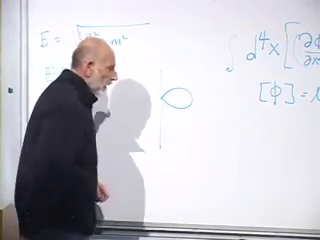
\includegraphics[width=0.72\textwidth]{lecture_03_figure_02.png}
\lectureframe{00:28:30.560}

\medskip
\begin{tikzpicture}[line width=0.8pt,scale=1.0]
  \draw[dashed] (-2.6,0) -- (0,0) -- (2.6,0);
  \fill (0,0) circle (0.055);
  \draw (0,0) .. controls (-0.85,0.7) and (-0.85,1.6) .. (0,1.6)
                .. controls (0.85,1.6) and (0.85,0.7) .. (0,0);
\end{tikzpicture}
\caption{La pizarra durante la transición a la autoenergía escalar, seguida de un redibujo esquemático prudente de la topología del tadpole. La captura muestra claramente el lazo, las fórmulas relativista y sin masa de la energía, y una parte de la acción; no se afirma que los coeficientes y rótulos ocultos sean visibles.}
\end{figure}

En el vértice, el escalar puede absorberse y reemitirse mientras las otras dos patas se propagan desde el punto de vuelta a sí mismo. Salvo factores numéricos y combinatorios, la corrección es
\begin{equation}
\delta m_\phi^2\sim \lambda G_\phi(0).
\end{equation}
El propagador en puntos coincidentes es infinito en la aproximación del continuo. Una teoría efectiva no pretende ser válida a distancias arbitrariamente cortas, así que imponemos \(|\Delta|\geq\delta\). Entonces,
\begin{equation}
G_\phi(0)\longrightarrow G_\phi(\delta)sim\frac{1}{\delta^2},
\qquad
\delta m_\phi^2\sim\frac{\lambda}{\delta^2}sim\lambda\Lambda^2.
\end{equation}
Se llama cuadrática a la divergencia porque contiene dos potencias del corte de momento. La integración en el espacio de momentos lleva a la misma conclusión: la contribución excesiva procede de momentos de lazo arbitrariamente grandes. Que la escala mínima quede determinada finalmente por la gran unificación, la gravedad cuántica o algo aún inimaginado no cambia el diagnóstico de la teoría efectiva.

Este es un problema de ajuste fino. Si \(\delta\) es extremadamente pequeño y \(\lambda\) no es extraordinariamente diminuto, la corrección radiativa es mucho mayor que la masa al cuadrado del escalar observada a bajas energías. Por tanto, el coeficiente desnudo y la corrección de lazo deben cancelarse hasta un número implausible de cifras:
\begin{equation}
m_{\mathrm{physical}}^2
=m_{\mathrm{bare}}^2+\delta m_\phi^2.
\end{equation}
El propagador masivo no resuelve la situación. A las distancias responsables de la divergencia, \(e^{-m|\Delta|}\simeq1\). El lazo ultravioleta ha dejado de depender de la masa mucho antes de alcanzar el corte.

\section{Dimensiones de los fermiones y su propagador}

Repitamos ahora el mismo análisis dimensional para un fermión de Dirac. Su acción libre es
\begin{equation}
S_\psi=\int d^4x\,
\bar\psi\left(i\gamma^\mu\partial_\mu-m\right)\psi.
\end{equation}
Las matrices gamma son numéricas y adimensionales. El término cinético contiene una sola derivada, así que
\begin{align}
1
&=L^4[\bar\psi]L^{-1}[\psi],\\
[\psi]=[\bar\psi]&=L^{-3/2}.
\end{align}
Las potencias semienteras no deberían alarmarnos: los fermiones introducen mitades en muchos lugares.

\begin{classroomqa}
\audiencequestion{¿No sería más fácil deducir \([\psi]\) a partir del término de masa? \lecturetimestamp{00:36:02}}
\lecturerresponse{Sí. El término de masa da \(L^4L^{-1}[\bar\psi\psi]=1\), de donde se obtiene \([\bar\psi\psi]=L^{-3}\) y \([\psi]=L^{-3/2}\). Primero usamos la derivación a partir del término cinético porque sigue siendo válida en la teoría sin masa y muestra por qué la masa del fermión aparece como \(m\), y no como \(m^2\).}
\end{classroomqa}

Dos campos fermiónicos tienen dimensión \(L^{-3}\), así que la abreviatura dimensional de la clase para el propagador sin masa es
\begin{equation}
S(\Delta)\sim\frac{1}{|\Delta|^3}.
\end{equation}
Al restituir su estructura matricial, se obtiene el numerador más preciso que exige la covariancia de Lorentz:
\begin{equation}
S_{ij}(\Delta)
\propto
\frac{\left(\gamma_\mu\Delta^\mu\right)_{ij}}
{\left(\Delta^2\right)^2}.
\end{equation}
El numerador añade una potencia de longitud, y el denominador contiene, por tanto, cuatro potencias del intervalo; la dimensión neta sigue siendo \(L^{-3}\). Al igual que en el caso escalar, la masa del fermión suprime el propagador a grandes separaciones, pero deja inalterado este escalamiento a corta distancia.

\section{Por qué un lazo fermiónico cerrado es negativo}

Ahora podemos preguntarnos si un diagrama fermiónico podría cancelar la autoenergía bosónica problemática. El tadpole escalar tiene signo positivo, salvo factores numéricos positivos como potencias de \(\pi\) y coeficientes combinatorios. Un lazo fermiónico cerrado tiene el signo opuesto.

\begin{classroomqa}
\audiencequestion{¿El signo menos del lazo fermiónico está relacionado con la explicación anterior de una rotación completa? \lecturetimestamp{00:40:21}}
\lecturerresponse{Forma parte de la misma estructura de signos fermiónica, pero aquí la demostración útil se basa en la antisimetría de intercambio, no en la orientación geométrica del lazo. Cortemos dos lazos, intercambiemos las partículas idénticas y volvamos a conectarlos. El intercambio convierte dos lazos en uno y aporta un signo menos solo para los fermiones.}
\end{classroomqa}

Vale la pena desarrollar el argumento completo. Supongamos que un diagrama de un lazo tiene signo \(\sigma\), positivo o negativo. Dos lazos idénticos y desconectados tienen signo
\begin{equation}
\sigma^2=+1.
\end{equation}
Cortemos simultáneamente ambos lazos. Ahora tenemos dos partículas idénticas que se propagan entre los cortes. Su función de onda ordinaria de dos partículas es simétrica para los bosones y antisimétrica para los fermiones:
\begin{align}
\Psi_B(x_1,x_2)&=+\Psi_B(x_2,x_1),\\
\Psi_F(x_1,x_2)&=-\Psi_F(x_2,x_1).
\end{align}
La antisimetría también explica el principio de exclusión de Pauli: si ambos fermiones ocupan el mismo estado, el intercambio no cambia nada físicamente, pero debe invertir la función de onda, que por tanto ha de anularse.

Volvamos a conectar las líneas cortadas después de intercambiar las dos partículas. Topológicamente, los dos lazos se han convertido en uno. La amplitud de los dos lazos sin intercambiar era positiva. El intercambio la deja positiva para los bosones y cambia su signo para los fermiones. Por tanto,
\begin{equation}
\begin{aligned}
\operatorname{sign}(\text{closed boson loop})&=+1,\\
\operatorname{sign}(\text{closed fermion loop})&=-1.
\end{aligned}
\end{equation}
La conclusión es general: cada lazo fermiónico cerrado independiente aporta un factor de \(-1\).

\section{El lazo de Yukawa}

Volvamos a la masa del escalar. Un bosón no puede convertirse en un solo fermión porque cambiaría la paridad del número fermiónico. La corrección fermiónica más sencilla consiste en que el escalar se divida en un par de fermión y antifermión, que se propagan formando un lazo y vuelven a recombinarse. La interacción es un acoplamiento de Yukawa,
\begin{equation}
\mathcal L_Y=-g\phi\bar\psi\psi.
\end{equation}
En el caso del Higgs, los fermiones pueden ser quarks o leptones. Hay dos puntos de interacción y, por tanto, dos factores de \(g\).

El tadpole escalar implicaba un solo punto, cuya posición global podía fijarse porque la invariancia traslacional solo aporta el volumen del espacio-tiempo. El lazo de Yukawa implica dos puntos. Podemos fijar uno de ellos o, de forma equivalente, fijar la posición media de ambos, pero debemos integrar sobre su separación relativa \(\Delta\). Cada propagador fermiónico aporta el factor de corta distancia \(1/|\Delta|^3\), así que
\begin{equation}
\delta m_{\phi,F}^2
\sim
-g^2\int_{|\Delta|\geq\delta}d^4\Delta\,
\frac{1}{|\Delta|^6}.
\end{equation}

Una vez escritos los dos propagadores, la integral sobre la separación y los dos acoplamientos, se pide a la clase un último factor. La respuesta es el signo menos. Los dos propagadores se cierran formando un lazo fermiónico, así que la integral de corta distancia, positiva en todo lo demás, queda multiplicada por \(-1\).

El análisis dimensional ya determina la divergencia. La medida \(d^4\Delta\) aporta cuatro potencias de longitud, hay seis en el denominador y la única escala de longitud restante es el corte:
\begin{equation}
\int_{|\Delta|\geq\delta}
\frac{d^4\Delta}{|\Delta|^6}
\sim\frac{1}{\delta^2}.
\end{equation}
Esto puede hacerse explícito con coordenadas radiales euclídeas en cuatro dimensiones:
\begin{equation}
\int_{\delta}^{R}d^4\Delta\,\frac{1}{|\Delta|^6}
=2\pi^2\int_{\delta}^{R}dr\,\frac{r^3}{r^6}
=\pi^2\left(\frac{1}{\delta^2}-\frac{1}{R^2}\right).
\end{equation}
Las trazas espinoriales y las normalizaciones de los propagadores modifican el coeficiente, pero no la dependencia cuadrática del corte.\editorialnote{La integral radial es una versión explícita estándar de la estimación dimensional hecha en la clase. Está escrita en términos de la distancia euclídea, donde la positividad y el conteo de potencias ultravioletas son transparentes.}

\begin{classroomqa}
\audiencequestion{¿Cambiaría el signo invertir o elegir otros límites de integración? \lecturetimestamp{00:51:06}}
\lecturerresponse{No. No se trata de una integral unidimensional orientada cuyos límites generen el signo físico. Es una integral sobre cuatro componentes o, de manera más clara, sobre una medida radial positiva. Su contribución ultravioleta es positiva. La contribución negativa procede únicamente del lazo fermiónico cerrado.}
\end{classroomqa}

\begin{classroomqa}
\audiencequestion{¿Cuál es la dimensión del acoplamiento de Yukawa \(g\)? \lecturetimestamp{00:51:51}}
\lecturerresponse{Es adimensional en cuatro dimensiones. Como \([\phi]=L^{-1}\) y \([\bar\psi\psi]=L^{-3}\), el producto \(\phi\bar\psi\psi\) tiene dimensión \(L^{-4}\), que queda exactamente compensada por \(d^4x\).}
\end{classroomqa}

La corrección fermiónica dominante es, por tanto,
\begin{equation}
\delta m_{\phi,F}^2
\sim -C_F\frac{g^2}{\delta^2}
=-C_Fg^2\Lambda^2,
\end{equation}
donde \(C_F>0\) contiene factores numéricos, espinoriales y de multiplicidad. El lazo escalar tiene la forma correspondiente
\begin{equation}
\delta m_{\phi,B}^2
\sim+C_B\frac{\lambda}{\delta^2}
=+C_B\lambda\Lambda^2.
\end{equation}
Aún no hemos resuelto el problema del ajuste fino, pero hemos encontrado algo indispensable: una contribución con el mismo grado de divergencia ultravioleta y signo opuesto.

\section{Qué exige la cancelación}

Sería una coincidencia extraordinaria que acoplamientos sin relación entre sí satisficieran
\begin{equation}
C_B\lambda=C_Fg^2
\end{equation}
con la precisión exacta que exige una gran jerarquía de escalas. La clase lo abrevia como \(g^2=\lambda\), omitiendo factores dependientes de las convenciones y de las multiplicidades. Una solución genuina requiere una estructura matemática que imponga la relación, no que se limite a permitirla.

Esa es la motivación de la supersimetría. La supersimetría relaciona bosones y fermiones y restringe sus acoplamientos a combinaciones que cancelan muchos términos divergentes que, de otro modo, serían problemáticos. La cancelación se repite entonces en todos los diagramas porque se deriva de una simetría, no de un ajuste de parámetros hecho lazo a lazo.

La coincidencia de masas también importa. Si las masas del bosón y del fermión son idénticas, sus propagadores completos pueden emparejarse con mayor precisión. Si las masas difieren ligeramente, las respuestas finitas completas no se cancelan de manera exacta, porque los propagadores difieren a distancias comparables con sus longitudes de Compton. Sin embargo, sus comportamientos asintóticos comunes a corta distancia pueden cancelar la parte divergente:
\begin{equation}
\mathcal I_B(\Delta)-\mathcal I_F(\Delta)
\quad\hbox{may be finite as}\quad \Delta\to0,
\end{equation}
donde \(\mathcal I_B\) y \(\mathcal I_F\) denotan los integrandos completos de los lazos bosónico y fermiónico, una vez incluidos los vértices, los numeradores y las multiplicidades. No se restan directamente los propagadores, que tienen dimensiones distintas. Aunque se cancelen los términos ultravioletas, puede quedar un residuo finito. Esto abre la posibilidad de una supersimetría aproximada o rota. La igualdad exacta produce la cancelación más limpia; una ruptura suficientemente controlada aún puede eliminar la catástrofe ultravioleta y dejar desdoblamientos de masa observables.

Así pues, hemos llegado a la supersimetría sin escribir todavía su álgebra. La cadena de razonamiento está completa:
\begin{equation}
\begin{gathered}
G_\phi(\Delta)\sim \Delta^{-2},
\qquad
\delta m_{\phi,B}^2\sim+C_B\lambda\Lambda^2,\\[0.4em]
S_\psi(\Delta)\sim \Delta^{-3},
\qquad
\delta m_{\phi,F}^2\sim-C_Fg^2\Lambda^2,\\[0.4em]
\text{symmetry-enforced matching}\\
\Longrightarrow\quad
\text{quadratic divergences cancel}.
\end{gathered}
\end{equation}
La tarea siguiente es entender el principio de simetría abstracto que impone esas relaciones y examinar ejemplos concretos de cómo actúa.
\chapter{De la simetría ordinaria al álgebra de Grassmann}

\lectureoverview{La supersimetría es una simetría, así que empezaremos por recordar qué significa esa palabra en mecánica cuántica. Una transformación física se representa en el espacio de Hilbert mediante un operador unitario; las transformaciones continuas se generan infinitesimalmente y sus conmutadores codifican cómo se componen. Una simetría genuina conserva la energía, lo que equivale a conmutar con el hamiltoniano. La supersimetría modifica entonces una hipótesis común a todos los ejemplos conocidos: sus generadores transforman bosones en fermiones y fermiones en bosones. Construir tales generadores conduce de forma natural a operadores de creación y aniquilación, anticonmutadores y el álgebra finita de Grassmann, en la que las cantidades impares se elevan al cuadrado y dan cero.}

\section{La simetría relaciona configuraciones distintas}

Una simetría no es una mera regularidad decorativa. Es una operación que relaciona una configuración física con otra. La reflexión izquierda-derecha, por ejemplo, relaciona las dos manos. Si la persona y las leyes que la rodean tuvieran una simetría exacta izquierda-derecha, las propiedades correspondientes de ambas manos coincidirían. En términos más generales, los objetos o estados relacionados por una simetría exacta deben compartir las magnitudes físicas que esta conserva. En física de partículas, eso suele significar que tienen masas iguales; en física atómica, que los estados de un mismo multiplete rotacional tienen las mismas energías.

Nuestro objetivo es la supersimetría, pero conviene recordar primero simetrías continuas como las rotaciones y las traslaciones. Ya resulta incómodo preguntar si la supersimetría es «continua» en el sentido habitual. Sus parámetros infinitesimales no son números reales ordinarios que conmuten. Es mejor entenderla como una extensión graduada de la simetría continua, y la aritmética de Grassmann que introduciremos a continuación precisa esa idea lo suficiente para nuestros fines. \editorialnote{La terminología moderna describe la supersimetría como una simetría continua graduada. Esta precisión explica la advertencia de la clase: la distinción habitual entre continuo y discreto no se aplica limpiamente a la supersimetría.}

\section{Operaciones unitarias en el espacio de Hilbert}

Un sistema cuántico se representa mediante un vector de estado \(\ket{\psi}\). Una operación de simetría física se representa mediante un operador \(U\) que actúa sobre ese estado:
\begin{equation}
\ket{\psi}\longmapsto U\ket{\psi}.
\end{equation}
En una rotación espacial, el eje y el ángulo determinan \(U\). Si un estado contiene partículas en varias posiciones, el ket transformado representa todas ellas en sus posiciones rotadas. Con una traslación ocurre algo parecido: el estado se transforma en otro que representa la configuración completa desplazada.

\begin{classroomqa}
\audiencequestion{El vector de estado pertenece a un espacio de Hilbert que a menudo es infinito-dimensional. ¿Estamos rotando el espacio de Hilbert o el espacio tridimensional ordinario? \lecturetimestamp{00:04:20}}
\lecturerresponse{Ambas descripciones se refieren a la misma operación en niveles distintos. La transformación unitaria actúa sobre el vector del espacio de Hilbert y representa la rotación física de la configuración en el espacio ordinario. No es literalmente una rotación tridimensional del espacio de Hilbert abstracto; es la representación de una rotación espacial en ese espacio.}
\end{classroomqa}

La condición esencial es la unitariedad:
\begin{equation}
U^\dagger U=UU^\dagger=\mathbf 1,
\qquad
U^{-1}=U^\dagger.
\end{equation}
Esta conserva los productos internos y, por tanto, las probabilidades:
\begin{equation}
\braket{U\psi}{U\psi}
=\bra{\psi}U^\dagger U\ket{\psi}
=\braket{\psi}{\psi}.
\end{equation}

\begin{figure}[H]
\centering
\includegraphics[width=0.56\textwidth]{lecture_04_figure_02.png}
\lectureframe{00:05:56.420}
\caption{Transición inicial en la pizarra desde un estado transformado hasta la condición de unitariedad. Se ven el ket y el producto con el operador adjunto, pero el profesor tapa sus extremos derechos; las ecuaciones completas aparecen en la derivación siguiente.}
\end{figure}

En sentido estricto, el teorema de Wigner también permite simetrías antiunitarias, como la inversión temporal. Las transformaciones conectadas continuamente con la identidad, que son las que nos ocupan aquí, se representan mediante operadores unitarios. \editorialnote{La posibilidad antiunitaria es una precisión habitual; no altera el análisis de los generadores de rotaciones, traslaciones o supersimetría que hacemos aquí.}

\section{Transformaciones infinitesimales y generadores}

La operación de no hacer nada se representa mediante \(U=\mathbf 1\), no mediante \(U=0\). Una transformación suficientemente pequeña difiere de la identidad en un término lineal en su parámetro pequeño. Para una rotación de ángulo pequeño \(\epsilon\),
\begin{equation}
U(\epsilon)=\mathbf 1+i\epsilon L+O(\epsilon^2).
\end{equation}
La unitariedad, al primer orden, exige
\begin{align}
U^\dagger U
&=\left(\mathbf 1-i\epsilon L^\dagger\right)
  \left(\mathbf 1+i\epsilon L\right)+O(\epsilon^2)\\
&=\mathbf 1+i\epsilon(L-L^\dagger)+O(\epsilon^2),
\end{align}
y, por tanto,
\begin{equation}
L^\dagger=L.
\end{equation}
El operador \(L\) es el generador infinitesimal.

Las rotaciones requieren tres generadores, uno por cada eje independiente:
\begin{equation}
L_x,\qquad L_y,\qquad L_z.
\end{equation}
Una rotación alrededor de un eje arbitrario \(\widehat{\bm n}\) está generada por
\begin{equation}
L_{\widehat{\bm n}}=\widehat{\bm n}\cdot\bm L.
\end{equation}

\begin{classroomqa}
\audiencequestion{¿Se pueden sumar los generadores de los ejes \(x\), \(y\) y \(z\) para obtener una rotación alrededor de otro eje? \lecturetimestamp{00:07:50}}
\lecturerresponse{Sí. Sus combinaciones lineales generan rotaciones alrededor de ejes intermedios. Tres componentes independientes bastan para construir cualquier rotación espacial infinitesimal.}
\end{classroomqa}

En el caso de las rotaciones, estos generadores son las componentes del momento angular. Esta notación resulta útil en términos más generales, porque toda simetría continua se describe localmente mediante sus generadores.

\section{El conmutador como tabla de multiplicar}

Los generadores de rotación satisfacen
\begin{align}
[L_x,L_y]&=iL_z,&
[L_y,L_z]&=iL_x,&
[L_z,L_x]&=iL_y,
\end{align}
o, de forma compacta,
\begin{equation}
[L_i,L_j]=i\epsilon_{ijk}L_k.
\end{equation}
El símbolo de Levi-Civita se anula si dos índices coinciden y vale \(+1\) o \(-1\) para permutaciones pares o impares de \(1,2,3\). El hecho estructural importante es el cierre: el conmutador de dos generadores es otro generador.

¿Por qué un conmutador describe la geometría de las rotaciones? Hagamos una rotación pequeña alrededor de \(x\), seguida de otra alrededor de \(y\); deshagamos la rotación alrededor de \(x\) y, por último, la rotación alrededor de \(y\). Las operaciones no se cancelan porque las rotaciones alrededor de ejes distintos no conmutan.

\begin{classroomqa}
\audiencequestion{¿Se puede ilustrar esta falta de conmutatividad con los movimientos de alabeo, cabeceo y guiñada de un avión? \lecturetimestamp{00:12:36}}
\lecturerresponse{Sí. Las rotaciones sucesivas alrededor de los ejes del cuerpo muestran de inmediato, desde el punto de vista geométrico, que cambiar el orden cambia la orientación final. El álgebra que veremos a continuación es la versión infinitesimal de ese hecho conocido.}
\end{classroomqa}

Sea
\begin{equation}
U_x(\epsilon)=\mathbf 1+i\epsilon L_x,
\qquad
U_y(\delta)=\mathbf 1+i\delta L_y.
\end{equation}
Como los operadores actúan sobre los kets de derecha a izquierda, la secuencia indicada se representa mediante
\begin{equation}
\mathcal C
=U_y^{-1}(\delta)U_x^{-1}(\epsilon)
 U_y(\delta)U_x(\epsilon).
\end{equation}

\begin{classroomqa}
\audiencequestion{¿Por qué se pueden escribir las operaciones inversas como inversas y no como adjuntas? \lecturetimestamp{00:13:25}}
\lecturerresponse{Porque las transformaciones son unitarias: \(U^\dagger=U^{-1}\). Para una transformación infinitesimal, tomar la inversa simplemente cambia el signo del término de primer orden: \(U_x^{-1}=\mathbf 1-i\epsilon L_x+O(\epsilon^2)\).}
\end{classroomqa}

Multiplicar los cuatro factores en la pizarra se convirtió en un ejercicio animado: se cancelaron todos los términos lineales en \(\epsilon\) o \(\delta\), la clase siguió los términos mixtos y una confusión momentánea con el factor dos mostró lo fácil que es perder de vista el orden de los operadores. El resultado limpio de segundo orden es
\begin{align}
\mathcal C
&=\mathbf 1+\epsilon\delta[L_x,L_y]
  +O(\epsilon^2\delta,\epsilon\delta^2)\\
&=\mathbf 1+i\epsilon\delta L_z
  +O(\epsilon^2\delta,\epsilon\delta^2).
\end{align}
Así, la secuencia cerrada deja una pequeña rotación alrededor de \(z\), con un ángulo proporcional a \(\epsilon\delta\). \editorialnote{La multiplicación mostrada fija el orden y el coeficiente tras el cálculo exploratorio hecho en clase. Invertir la convención de la secuencia cambia el signo, pero no la conclusión: la transformación residual está regida por el conmutador.}

\begin{classroomqa}
\audiencequestion{¿Cambiar el orden de las operaciones inversas haría que el producto fuese la identidad? \lecturetimestamp{00:25:23}}
\lecturerresponse{Si cada transformación se coloca inmediatamente junto a su propia inversa, los pares se cancelan. La secuencia no trivial del conmutador separa deliberadamente esos pares; el hecho de que no se reduzca a la identidad mide la dependencia del orden.}
\end{classroomqa}

Los productos más largos sí se vuelven más complicados, pero no contienen ningún principio nuevo.

\begin{classroomqa}
\audiencequestion{¿Qué ocurre si hay más de tres generadores o muchas transformaciones pequeñas? \lecturetimestamp{00:25:34}}
\lecturerresponse{Hay más conmutadores y más cuentas, pero conocer el álgebra cerrada permite determinar cómo se combinan un número arbitrario de transformaciones infinitesimales. Las transformaciones finitas se pueden construir a partir de muchas transformaciones pequeñas.}
\end{classroomqa}

En este sentido, el álgebra de conmutadores es la tabla de multiplicar de un grupo continuo escrita en las proximidades de la identidad.

\section{Las traslaciones completan el ejemplo espacial}

El momento lineal genera las traslaciones espaciales. Con la convención de signos usada en la clase,
\begin{equation}
\begin{aligned}
T_x(a)&=\mathbf 1+iaP_x+O(a^2),\\
T_y(b)&=\mathbf 1+ibP_y+O(b^2),
\end{aligned}
\end{equation}
donde \(a\) y \(b\) son distancias, no ángulos.

Dos traslaciones conmutan. Desplacemos un punto en la dirección \(x\), luego en la dirección \(y\), deshagamos la traslación en la dirección \(x\) y, por último, la traslación en la dirección \(y\); el punto vuelve a su origen:
\begin{equation}
[P_i,P_j]=0.
\end{equation}

\begin{classroomqa}
\audiencequestion{¿Para trasladar o rotar un objeto físico hacen falta fuerzas que inicien y detengan el movimiento? \lecturetimestamp{00:28:45}}
\lecturerresponse{Esa no es la operación que estamos definiendo. Una transformación de simetría compara el estado original con el estado matemático en el que se ha desplazado o rotado la configuración entera. No describe una trayectoria dinámica, una aceleración ni el trabajo realizado al mover el aparato.}
\end{classroomqa}

Una rotación y una traslación no conmutan. Traslademos un punto, rotemoslo alrededor del origen, trasladémoslo de vuelta a lo largo del eje original y deshagamos la rotación; el punto no vuelve a su posición inicial. El álgebra mixta es
\begin{equation}
[L_i,P_j]=i\epsilon_{ijk}P_k.
\end{equation}
Esta relación indica que el momento lineal se transforma como un vector bajo rotaciones. Aquí importa menos el ejercicio concreto con los índices que la lección general: las transformaciones del espacio euclídeo se codifican en los conmutadores entre los generadores de rotaciones y traslaciones.

\section{Una simetría debe conservar la energía}

Pasemos ahora de la composición de transformaciones a la dinámica. Si \(U\) es realmente una simetría de un sistema, aplicarla no puede cambiar la energía. Sea \(\ket{E}\) un estado propio de la energía:
\begin{equation}
H\ket{E}=E\ket{E}.
\end{equation}
El símbolo \(E\) de la derecha es un número; \(\ket{E}\) es un vector etiquetado por ese valor propio.

\begin{figure}[H]
\centering
\begin{minipage}[t]{0.43\textwidth}
\centering
\includegraphics[width=\linewidth]{lecture_04_figure_03.png}
\lectureframe{00:34:38.239}
\end{minipage}
\hfill
\begin{minipage}[t]{0.50\textwidth}
\centering
\includegraphics[width=\linewidth]{lecture_04_figure_04.png}
\lectureframe{00:36:22.376}
\end{minipage}
\caption{El ket transformado \(U\ket{E}\) y la ecuación que define el estado propio \(H\ket{E}=E\ket{E}\), aislados en fotogramas sucesivos de la pizarra.}
\end{figure}

Si \(U\) es una simetría, entonces \(U\ket{E}\) tiene el mismo valor propio:
\begin{equation}
HU\ket{E}=EU\ket{E}.
\end{equation}
Como \(E\) es un escalar, conmuta con \(U\), y podemos usar la ecuación original del estado propio:
\begin{align}
HU\ket{E}
&=EU\ket{E}\\
&=UE\ket{E}\\
&=UH\ket{E}.
\end{align}
Por tanto,
\begin{equation}
(HU-UH)\ket{E}=0.
\end{equation}

\begin{classroomqa}
\audiencequestion{¿Se puede repetir la derivación desde la primera relación? \lecturetimestamp{00:35:55}}
\lecturerresponse{Partamos de \(H\ket{E}=E\ket{E}\). La simetría implica que \(U\ket{E}\) tiene la misma energía, de modo que \(HU\ket{E}=EU\ket{E}\). Pasemos el escalar \(E\) a través de \(U\), sustituyamos \(E\ket{E}\) por \(H\ket{E}\) y restemos. El resultado es \((HU-UH)\ket{E}=0\).}
\end{classroomqa}

\begin{figure}[H]
\centering
\includegraphics[width=0.70\textwidth]{lecture_04_figure_05.png}
\lectureframe{00:38:51.066}
\caption{La derivación completa en la pizarra. Unas marcas curvas de guía conectan la igualdad de energías con la sustitución \(E\ket{E}=H\ket{E}\); la última línea es \((HU-UH)\ket{E}=0\).}
\end{figure}

El argumento vale para todos los estados propios de la energía. Si suponemos que esos estados forman una base completa, un operador que anula cada uno de ellos es el operador nulo:
\begin{equation}
[H,U]=0.
\end{equation}
Este es el criterio para que una transformación unitaria independiente del tiempo sea una simetría del hamiltoniano.

Para una transformación infinitesimal,
\begin{equation}
U(\epsilon)=\mathbf 1+i\epsilon L_i+O(\epsilon^2),
\end{equation}
la identidad ya conmuta con \(H\), así que cada generador debe satisfacer
\begin{equation}
[L_i,H]=0.
\end{equation}

\begin{figure}[H]
\centering
\includegraphics[width=0.47\textwidth]{lecture_04_figure_06.png}
\lectureframe{00:42:14.296}
\caption{Criterio de simetría resumido en la pizarra: \([U,H]=0\), seguido de su forma para los generadores, normalizada a partir de la etiqueta inferior parcialmente borrosa como \([L_i,H]=0\).}
\end{figure}

Si \(L_i\) no depende explícitamente del tiempo, la ecuación de Heisenberg da
\begin{equation}
\frac{dL_i}{dt}
=i[H,L_i]=0
\qquad(\hbar=1).
\end{equation}
Por tanto, los generadores de simetría son cargas conservadas. La simetría de traslación espacial implica la conservación del momento lineal; la simetría de rotación, la conservación del momento angular. \editorialnote{La condición de que no haya dependencia temporal explícita es una precisión habitual e implícita en la afirmación de la clase sobre las leyes de conservación.}

\section{Transformar todo el sistema físico}

La expresión «la rotación es una simetría» puede usarse mal si solo se transforma una parte del aparato. Se puede rotar el espín de una partícula libre sin cambiar su energía. Pero si se coloca en un campo magnético fijo y se rota solo el espín, su energía de Zeeman cambia. Eso no refuta la simetría de rotación: significa que el campo se mantuvo fijo mientras el espín se rotaba con respecto a él. Si se rotan juntos el espín y el campo, o se usa un campo externo que sea invariante por sí mismo, la energía no cambia.

Lo mismo sucede en un átomo de hidrógeno. Trasladar solo el electrón con respecto al protón cambia la distancia entre ambos y, por tanto, la energía de Coulomb. La simetría de traslación actúa sobre el sistema electrón-protón completo y desplaza ambos en la misma medida.

\begin{classroomqa}
\audiencequestion{¿Es necesario que el campo externo tenga la simetría? \lecturetimestamp{00:43:09}}
\lecturerresponse{El campo externo fijo debe ser invariante bajo la operación, o bien debe transformarse junto con el resto del sistema. Una rotación relativa entre un espín y un campo que no se ha rotado da lugar a una configuración física distinta, no a la transformación de simetría del montaje completo.}
\end{classroomqa}

La degeneración rotacional de un átomo ofrece un ejemplo positivo claro. Para un momento angular fijo \(l\), las rotaciones mezclan estados con números cuánticos magnéticos
\begin{equation}
m=-l,-l+1,\ldots,l.
\end{equation}
En ausencia de un campo magnético o eléctrico externo, todos los estados del multiplete tienen la misma energía:
\begin{equation}
E_{l,m}=E_l.
\end{equation}
La simetría relaciona estados distintos y exige que sean degenerados.

\section{Qué cambia con la supersimetría}

Todas las simetrías conocidas que hemos comentado hasta ahora conservan el carácter bosónico o fermiónico. Una rotación transforma un electrón en otro electrón, no en un fotón. Las rotaciones de color mezclan los tres colores de un quark, pero no lo convierten en un gluón. Las simetrías internas y espaciotemporales ordinarias pueden mezclar componentes o etiquetas cuánticas, pero sus generadores son bosónicos y no cambian la paridad fermiónica.

La supersimetría es distinta:
\begin{equation}
Q\ket{B}\sim\ket{F},
\qquad
Q\ket{F}\sim\ket{B}.
\end{equation}
Sus multipletes cruzan la frontera entre bosones y fermiones. En una teoría supersimétrica exacta, los compañeros de un mismo multiplete tienen la misma masa. Este es precisamente el emparejamiento que necesitábamos de las clases anteriores: los lazos bosónicos y fermiónicos emparejados pueden cancelar las grandes correcciones ultravioleta a las masas de los escalares. La construcción es difícil de visualizar porque ningún movimiento espacial ordinario transforma un estado de espín entero en uno de espín semientero. Por eso procederemos algebraicamente.

\section{Una supercarga prototípica}

Sea \(A,A^\dagger\) el operador que aniquila y crea un bosón, y sea \(C,C^\dagger\) el que aniquila y crea un fermión. El operador hermítico más sencillo que intercambia sus estados de una partícula es
\begin{equation}
Q=C^\dagger A+A^\dagger C.
\end{equation}
El primer término aniquila un bosón y crea un fermión; el segundo aniquila un fermión y crea un bosón. Si \(Q\) actúa sobre un estado de un bosón, el término \(A^\dagger C\) se anula porque no hay ningún fermión que aniquilar, mientras que \(C^\dagger A\) realiza la conversión. En un estado de un fermión ocurre al revés.

\begin{classroomqa}
\audiencequestion{¿Esta construcción crea una partícula única que es una superposición de un bosón y un fermión? \lecturetimestamp{00:52:37}}
\lecturerresponse{\(Q\) es un operador, no un estado. Al actuar sobre un estado puramente bosónico, produce un estado fermiónico; al actuar sobre uno puramente fermiónico, produce un estado bosónico. Si actúa linealmente sobre una superposición ya general, produce otra superposición, como hace cualquier operador lineal.}
\end{classroomqa}

La clase pone a prueba ahora el vacío. Como ambos operadores de aniquilación lo anulan,
\begin{equation}
A\ket{0}=0,\qquad C\ket{0}=0,
\end{equation}
tenemos
\begin{equation}
Q\ket{0}=0.
\end{equation}
El resultado es el vector nulo, no una segunda copia del vacío.

El modelo prototípico es deliberadamente esquemático. Un bosón de espín cero puede transformarse en cualquiera de las componentes de un fermión de espín un medio, así que el generador necesita un índice espinorial:
\begin{equation}
Q_\alpha\ket{B}\sim\ket{F_\alpha}.
\end{equation}
En la representación simplificada de dos componentes que usamos en la clase,
\begin{equation}
Q_\alpha\ket{F_\beta}\sim\delta_{\alpha\beta}\ket{B}.
\end{equation}

\begin{classroomqa}
\audiencequestion{¿Cómo pueden coincidir las dimensiones de los espacios de estados si un bosón de espín cero tiene una componente de espín y un fermión de espín un medio tiene dos? \lecturetimestamp{00:55:02}}
\lecturerresponse{Un \(Q\) sin índice no basta. Hay componentes espinoriales \(Q_\alpha\), cada una capaz de producir una componente de espín del fermión. La supercarga misma tiene espín un medio porque cambia el espín en media unidad.}
\end{classroomqa}

Las \(Q_\alpha\) son operadores fermiónicos o, más precisamente, impares de Grassmann. Cada uno de sus términos contiene un número impar de operadores fermiónicos, por lo que invierten la paridad fermiónica. Los observables medibles ordinarios son pares. Conviene distinguir una supercarga impar de su parámetro de transformación, también impar: una transformación supersimétrica finita se construye a partir de una combinación par como \(\epsilon^\alpha Q_\alpha+\bar\epsilon_{\dot\alpha}\bar Q^{\dot\alpha}\), en la que tanto \(\epsilon\) como \(Q\) son impares. \editorialnote{En la clase, el profesor llama informalmente números de Grassmann a los generadores. Más precisamente, las supercargas son operadores impares, mientras que los parámetros anticonmutativos son números de Grassmann; su producto es par y puede aparecer en una transformación finita.}

\section{Álgebras de operadores bosónicos y fermiónicos}

Para modos bosónicos etiquetados por \(i,j\),
\begin{align}
[A_i,A_j]&=0,&
[A_i^\dagger,A_j^\dagger]&=0,&
[A_i,A_j^\dagger]&=\delta_{ij}.
\end{align}
Las etiquetas pueden representar el momento, la posición, el espín o cualquier base completa de una partícula. Como los operadores de creación conmutan,
\begin{equation}
A_i^\dagger A_j^\dagger\ket{0}
=A_j^\dagger A_i^\dagger\ket{0}.
\end{equation}
El estado de dos bosones es simétrico al intercambiarlos.

Los operadores fermiónicos satisfacen relaciones de anticonmutación:
\begin{align}
\{C_i,C_j\}&=0,&
\{C_i^\dagger,C_j^\dagger\}&=0,&
\{C_i,C_j^\dagger\}&=\delta_{ij},
\end{align}
donde
\begin{equation}
\{X,Y\}=XY+YX.
\end{equation}
Para un solo modo,
\begin{equation}
\{C^\dagger,C^\dagger\}=2(C^\dagger)^2=0,
\end{equation}
y, por tanto,
\begin{equation}
(C^\dagger)^2=0.
\end{equation}
El operador no es nulo; su cuadrado sí lo es. Puede crear un fermión en ese modo, pero una segunda aplicación da cero. Esta es la exclusión de Pauli expresada en el lenguaje de operadores.

Para etiquetas distintas,
\begin{equation}
C_i^\dagger C_j^\dagger\ket{0}
=-C_j^\dagger C_i^\dagger\ket{0},
\end{equation}
que expresa la antisimetría del estado de dos fermiones. La sustitución algebraica
\begin{equation}
\begin{gathered}
\text{bosons: commutators}\\
\Updownarrow\\
\text{fermions: anticommutators}
\end{gathered}
\end{equation}
codifica la distinción estadística.

Muchos bosones pueden ocupar un mismo modo. Por eso, una gran ocupación de fotones puede comportarse como un campo electromagnético clásico con una amplitud numérica ordinaria. Los fermiones no pueden acumularse en un mismo modo, y un campo fermiónico impar no adquiere un valor clásico ordinario que conmute. Esto motiva una aritmética distinta para llevar la cuenta de los fermiones.

\section{Números de Grassmann y paridad}

Los números ordinarios conmutan:
\begin{equation}
\alpha_i\alpha_j=\alpha_j\alpha_i.
\end{equation}
Los generadores de Grassmann anticonmutan:
\begin{equation}
\theta_i\theta_j=-\theta_j\theta_i.
\end{equation}
Al imponer \(i=j\) en un sistema numérico donde \(2\neq0\), se obtiene
\begin{equation}
\theta_i^2=0.
\end{equation}
No se puede asignar a \(\theta_i\) ningún valor numérico ordinario, como seis o siete. Estos símbolos forman un álgebra diseñada para llevar la cuenta de los signos fermiónicos.

Los coeficientes ordinarios conmutan con los generadores de Grassmann:
\begin{equation}
\alpha\theta_i=\theta_i\alpha.
\end{equation}

\begin{classroomqa}
\audiencequestion{¿Qué tipo de objeto se obtiene al multiplicar un número ordinario por un número de Grassmann? \lecturetimestamp{01:12:32}}
\lecturerresponse{Sigue siendo impar de Grassmann. Multiplicar por un coeficiente ordinario cambia su escala, no su paridad. El espacio generado por los generadores es un espacio vectorial sobre los números ordinarios.}
\end{classroomqa}

El álgebra tiene paridad \(\mathbb Z_2\). Los coeficientes ordinarios y los productos de un número par de generadores son pares; un generador o un producto de un número impar de ellos es impar:
\begin{equation}
\begin{aligned}
\text{even}\cdot\text{even}&=\text{even},\\
\text{even}\cdot\text{odd}&=\text{odd},\\
\text{odd}\cdot\text{odd}&=\text{even}.
\end{aligned}
\end{equation}

\begin{classroomqa}
\audiencequestion{¿Es esto análogo a las reglas de multiplicación de los números reales e imaginarios, o una generalización como la introducción de \(i\)? \lecturetimestamp{01:14:25}}
\lecturerresponse{Es una generalización de la aritmética, pero no conviene llevar demasiado lejos la analogía. Los números imaginarios siguen conmutando y satisfacen \(i^2=-1\); las cantidades impares de Grassmann anticonmutan y se elevan al cuadrado dando cero. El hecho de compartir el patrón de multiplicación par-impar no hace que las álgebras sean iguales.}
\end{classroomqa}

Un producto como \(\theta_1\theta_2\) es par y conmuta con todo elemento homogéneo del álgebra de Grassmann, pero no es un número ordinario. No es nulo, aunque
\begin{equation}
(\theta_1\theta_2)^2=0.
\end{equation}

\begin{classroomqa}
\audiencequestion{Si \(\theta_1\theta_2\) es par, ¿por qué no es simplemente un número ordinario? \lecturetimestamp{01:17:36}}
\lecturerresponse{La paridad par significa que conmuta en el álgebra graduada; no significa que sea un escalar real o complejo. Su nilpotencia lo distingue de inmediato de cualquier número ordinario no nulo.}
\end{classroomqa}

\section{Funciones de variables de Grassmann}

Con un generador, todo polinomio termina en primer orden:
\begin{equation}
f(\theta)=\alpha+\beta\theta.
\end{equation}
Todas las potencias \(\theta^n\) con \(n\geq2\) se anulan. Con dos generadores, el elemento más general es
\begin{equation}
f(\theta_1,\theta_2)
=\alpha+\beta_1\theta_1+\beta_2\theta_2
+\gamma\theta_1\theta_2.
\end{equation}
Escribir el último monomio en orden inverso cambia su signo:
\begin{equation}
\theta_2\theta_1=-\theta_1\theta_2.
\end{equation}

\begin{classroomqa}
\audiencequestion{¿Multiplicar \(\theta_1\) por un coeficiente \(\beta\) crea una tercera variable de Grassmann independiente? \lecturetimestamp{01:18:39}}
\lecturerresponse{No. Crea otro vector en el espacio generado por \(\theta_1\), no un nuevo generador de la base. Con dos generadores independientes, todo término lineal impar es de la forma \(\beta_1\theta_1+\beta_2\theta_2\).}
\end{classroomqa}

Con tres generadores, la base ordenada es
\begin{equation}
1,\quad
\theta_1,\theta_2,\theta_3,\quad
\theta_1\theta_2,\theta_1\theta_3,\theta_2\theta_3,\quad
\theta_1\theta_2\theta_3.
\end{equation}
En general, \(n\) generadores producen \(2^n\) monomios de base ordenados. Toda función analítica de un número finito de generadores de Grassmann se trunca en un polinomio de este tipo, porque las potencias repetidas de un mismo generador se anulan. \editorialnote{La base de dimensión \(2^n\) muestra explícitamente el patrón que la clase construye para uno, dos y tres generadores.}

\section{Derivación de Grassmann}

Para una variable, definamos
\begin{equation}
\frac{\partial}{\partial\theta}\alpha=0,
\qquad
\frac{\partial}{\partial\theta}\theta=1,
\end{equation}
de modo que
\begin{equation}
\frac{\partial}{\partial\theta}
(\alpha+\beta\theta)=\beta.
\end{equation}
Para dos variables, elijamos derivadas por la izquierda y conservemos el orden canónico \(\theta_1\theta_2\):
\begin{align}
\frac{\partial^L f}{\partial\theta_1}
&=\beta_1+\gamma\theta_2,\\
\frac{\partial^L f}{\partial\theta_2}
&=\beta_2-\gamma\theta_1.
\end{align}
El signo menos de la segunda línea aparece porque la derivada impar debe pasar por \(\theta_1\) antes de derivar respecto de \(\theta_2\).

Esto se expresa mediante la regla del producto graduada. Si \(A\) tiene paridad \(|A|\in\{0,1\}\), entonces
\begin{equation}
\frac{\partial^L}{\partial\theta}(AB)
=\left(\frac{\partial^L A}{\partial\theta}\right)B
+(-1)^{|A|}A
\left(\frac{\partial^L B}{\partial\theta}\right).
\end{equation}
La regla sigue el espíritu de la regla ordinaria, pero incorpora el signo requerido por la anticonmutación. También se puede definir la integración de Grassmann y, como el espacio de funciones es finito, se reduce a una tabla breve. En la clase se deja esa tabla para más adelante.

\section{Se resuelve el enigma de la exponencial}

Con un único generador de Grassmann y un coeficiente ordinario \(a\),
\begin{equation}
e^{a\theta}
=1+a\theta,
\end{equation}
porque todas las potencias superiores se anulan. Dos exponenciales que contienen el mismo generador satisfacen
\begin{align}
e^{a\theta}e^{b\theta}
&=(1+a\theta)(1+b\theta)\\
&=1+(a+b)\theta\\
&=e^{(a+b)\theta}.
\end{align}

A continuación, la clase prueba con generadores distintos. La multiplicación directa da
\begin{equation}
e^{\theta_1}e^{\theta_2}
=(1+\theta_1)(1+\theta_2)
=1+\theta_1+\theta_2+\theta_1\theta_2.
\end{equation}
Al principio, el desarrollo en la pizarra parece indicar que el cuadrado de \(\theta_1+\theta_2\) podría dar el último término. Alguien del público advierte el signo:
\begin{equation}
(\theta_1+\theta_2)^2
=\theta_1^2+\theta_1\theta_2
 +\theta_2\theta_1+\theta_2^2
=0.
\end{equation}

\begin{classroomqa}
\audiencequestion{¿Se cancela el término cuadrático porque contiene \(\theta_1\theta_2+\theta_2\theta_1\)? \lecturetimestamp{01:24:00}}
\lecturerresponse{Sí. Esa corrección cambia la conclusión: \(e^{\theta_1+\theta_2}=1+\theta_1+\theta_2\), mientras que el producto ordenado \(e^{\theta_1}e^{\theta_2}\) también contiene \(\theta_1\theta_2\). La ley ingenua de suma de exponentes no se aplica a exponentes distintos que anticonmutan.}
\end{classroomqa}

No hay contradicción. Incluso para matrices ordinarias, \(e^Ae^B=e^{A+B}\) solo se cumple cuando \(A\) y \(B\) conmutan. En este caso,
\begin{equation}
[\theta_1,\theta_2]
=\theta_1\theta_2-\theta_2\theta_1
=2\theta_1\theta_2.
\end{equation}
Este conmutador es par y conmuta con ambos generadores, así que la serie de Baker-Campbell-Hausdorff termina:
\begin{equation}
e^{\theta_1}e^{\theta_2}
=\exp\left(
\theta_1+\theta_2+\frac12[\theta_1,\theta_2]
\right)
=e^{\theta_1+\theta_2+\theta_1\theta_2}.
\end{equation}
Como el exponente de la derecha es nilpotente, su desarrollo da exactamente
\(1+\theta_1+\theta_2+\theta_1\theta_2\). \editorialnote{Este cálculo de Baker-Campbell-Hausdorff resuelve la cuestión que queda pendiente en la clase en directo. Allí se descubre correctamente que la ley ingenua falla, pero la clase termina antes de identificar el término de conmutador que falta.}

\begin{classroomqa}
\audiencequestion{¿Qué tipo de número es \(1+\theta_1\), y se pueden sumar partes ordinarias y de Grassmann? \lecturetimestamp{01:26:16}}
\lecturerresponse{Es un elemento no homogéneo del álgebra de Grassmann, con una parte par \(1\) y una parte impar \(\theta_1\). Se permiten esas sumas, pero no son ni escalares ordinarios ni elementos impares homogéneos.}
\end{classroomqa}

Hacia el final se examina otra aparente paradoja:
\begin{equation}
(\theta_1+\theta_2)^2=0.
\end{equation}
Esto no implica que \(\theta_1\theta_2=0\), porque los dos términos cruzados se cancelan entre sí, en lugar de anularse por separado.

\begin{classroomqa}
\audiencequestion{Si todo elemento impar de Grassmann se eleva al cuadrado y da cero, ¿significa eso que el producto de dos generadores de Grassmann cualesquiera es cero? \lecturetimestamp{01:32:19}}
\lecturerresponse{No. La ecuación \((\theta_1+\theta_2)^2=0\) dice que \(\theta_1\theta_2+\theta_2\theta_1=0\). Esto demuestra la anticonmutación, no que alguno de los dos productos ordenados se anule. El producto de generadores distintos puede ser distinto de cero.}
\end{classroomqa}

\begin{classroomqa}
\audiencequestion{¿Estamos suponiendo la definición habitual mediante series de potencias al escribir estas exponenciales? \lecturetimestamp{01:34:42}}
\lecturerresponse{Sí, y esa definición es coherente porque todas las series terminan. Lo que falla no es la exponencial en sí, sino la identidad injustificada \(e^Ae^B=e^{A+B}\) para \(A\) y \(B\) que no conmutan. La corrección con el conmutador restablece la ley de composición adecuada.}
\end{classroomqa}

Este final exploratorio es adecuado. Las simetrías ordinarias nos llevaron de las transformaciones unitarias a los generadores y los conmutadores; la supersimetría nos llevó de los generadores impares a las variables anticonmutativas. En ambos casos, la ley de multiplicación es el objeto central. Para las rotaciones aparece en \([L_i,L_j]\); para las exponenciales de Grassmann, aparece en el término con el conmutador, que impide la suma ingenua. El álgebra es poco familiar, pero es coherente, finita y exactamente la adecuada para las transformaciones fermiónicas que requiere la supersimetría.

\chapter{Supercargas, cierre y superspacio}

\lectureoverview{La supersimetría es difícil, no porque sus reglas sean numerosas, sino porque estas reúnen ideas que la física ordinaria mantiene separadas. Empezamos con variables de Grassmann, cuyos elementos impares anticonmutan y cuyas funciones se truncan tras un número finito de términos. El álgebra de sus derivadas proporciona entonces el modelo para los generadores de simetría impares. Un oscilador bosónico y uno fermiónico dan lugar a las supercargas más sencillas: su anticonmutador es el hamiltoniano, de modo que el intercambio de bosones y fermiones es inseparable de las traslaciones temporales. La misma álgebra puede representarse geométricamente mediante traslaciones en direcciones de Grassmann de un espacio-tiempo ampliado llamado superspacio.}

\section{Por qué hay que retroceder antes de avanzar}

La supersimetría es una de las construcciones más abstractas de la física. Se parece a las rotaciones y las traslaciones porque es una simetría, pero no cabe en el espacio-tiempo ordinario sin ampliar lo que entendemos por coordenada. Sus parámetros naturales son cantidades de Grassmann: objetos que pueden sumarse y multiplicarse, pero que anticonmutan en vez de conmutar.

Por eso no sería útil abordar directamente el álgebra final. Primero haremos manejable la aritmética impar; después recordaremos cómo se organizan las simetrías continuas ordinarias, y solo entonces combinaremos ambas ideas. El recorrido es más largo, pero cada paso prepara el siguiente.

\section{El álgebra de Grassmann en la práctica}

\subsection{Elementos impares y pares}

Sean \(\epsilon_i\) generadores independientes de Grassmann. Cumplen
\begin{equation}
\epsilon_i\epsilon_j=-\epsilon_j\epsilon_i,
\qquad
\{\epsilon_i,\epsilon_j\}=0.
\end{equation}
Al tomar \(i=j\) se obtiene
\begin{equation}
2\epsilon_i^2=0,
\qquad
\epsilon_i^2=0,
\end{equation}
sobre los números reales o complejos. El generador no es cero; solo su cuadrado es cero.

Cada elemento homogéneo tiene una paridad. Un producto que contiene un número impar de generadores de Grassmann es impar, mientras que uno que contiene un número par es par:
\begin{align}
\text{odd}\times\text{odd}&=\text{even},\\
\text{odd}\times\text{even}&=\text{odd},\\
\text{even}\times\text{even}&=\text{even}.
\end{align}
Los elementos pares conmutan con los elementos homogéneos. Dos elementos impares anticonmutan. Así,
\begin{equation}
n\epsilon_i=\epsilon_i n,
\qquad
\epsilon_i\epsilon_j=-\epsilon_j\epsilon_i,
\end{equation}
cuando \(n\) es par.

Un elemento par no tiene por qué ser un número real o complejo ordinario. Por ejemplo, el producto
\(\epsilon_1\epsilon_2\) es par y nilpotente. Los números ordinarios forman la parte escalar del álgebra, mientras que los productos pares aportan otros elementos conmutativos.

\begin{classroomqa}
\audiencequestion{¿Hay alguna diferencia entre el álgebra de Grassmann y los números de Grassmann, o son lo mismo? \lecturetimestamp{00:06:45}}
\lecturerresponse{Los elementos son los números de Grassmann; el álgebra es el conjunto de esos elementos junto con sus reglas de suma y multiplicación. Por tanto, puede hablarse informalmente del mismo objeto, pero es útil distinguir entre las entidades con las que se opera y las reglas que rigen esas operaciones.}
\end{classroomqa}

\subsection{Las funciones se truncan}

Una función de una variable de Grassmann solo puede contener dos potencias:
\begin{equation}
f(\epsilon)=a+b\epsilon.
\end{equation}
No hay término \(\epsilon^2\). Con dos generadores independientes,
\begin{equation}
f(\epsilon_1,\epsilon_2)
=a+b_1\epsilon_1+b_2\epsilon_2+c\epsilon_1\epsilon_2.
\end{equation}
el desarrollo termina cuando aparecen ambos generadores. Para \(n\) generadores independientes, los monomios ordenados forman una base de dimensión \(2^n\):
\begin{equation}
1,\quad
\epsilon_i,\quad
\epsilon_i\epsilon_j,\quad
\ldots,\quad
\epsilon_1\epsilon_2\cdots\epsilon_n.
\end{equation}
\editorialnote{El resultado finito en dimensión \(2^n\) es el patrón general que subyace a los ejemplos con uno y dos generadores. También puede definirse un álgebra de Grassmann infinita, pero todos los polinomios que usamos aquí contienen solo un número finito de generadores.}

Al combinar dos generadores reales en un par complejo \(\theta,\bar\theta\), una función general puede escribirse, con un orden elegido, como
\begin{equation}
f(\theta,\bar\theta)
=a+\bar b\,\theta+\bar\theta\,b+c\,\bar\theta\theta.
\end{equation}
La barra indica la notación de par complejo que usamos aquí. Invertir el orden final cambia el signo:
\begin{equation}
\bar\theta\theta=-\theta\bar\theta.
\end{equation}

Suele ser conveniente asignar una paridad definida a toda la función. Si \(f\) es par, entonces \(a\) y \(c\) son pares, mientras que \(b\) y \(\bar b\) son impares. Si \(f\) es impar, esas asignaciones se invierten. Los coeficientes pueden pertenecer a un álgebra de Grassmann más amplia, siempre que no dependan de las variables particulares respecto de las cuales desarrollamos la función.

\begin{classroomqa}
\audiencequestion{¿Se puede introducir una variable de Grassmann en funciones trigonométricas u otras funciones analíticas? \lecturetimestamp{00:11:06}}
\lecturerresponse{Sí, pero la serie de potencias se trunca enseguida. Para un generador impar,
\[
\sin\epsilon=\epsilon,\qquad
\cos\epsilon=1,\qquad
e^\epsilon=1+\epsilon.
\]
Se conservan los nombres habituales, pero hay tan pocas potencias que las funciones no pueden adquirir la complejidad analítica acostumbrada.}
\end{classroomqa}

\section{Derivar es llevar la cuenta de los signos}

Usaremos una derivada izquierda de Grassmann. Sus reglas locales definitorias son
\begin{equation}
\partial_\theta a=0,
\qquad
\partial_\theta(\theta B)=B,
\end{equation}
cuando \(a\) y \(B\) no dependen de \(\theta\). Antes de derivar, llevamos el \(\theta\) pertinente a la izquierda. Cada vez que pasa junto a otro factor impar, cambia el signo.

Por ejemplo, si \(b\) es impar,
\begin{equation}
b\theta=-\theta b,
\qquad
\partial_\theta(b\theta)=-b.
\end{equation}
No hay nada misterioso en la derivada. El signo menos apareció antes de derivar, al reordenar los factores impares.

\subsection{El cálculo con dos variables}

Volvamos a
\begin{equation}
f(\theta,\bar\theta)
=a+\bar b\,\theta+\bar\theta\,b+c\,\bar\theta\theta.
\end{equation}
Supongamos primero que \(f\) es par. Entonces \(\bar b\) es impar y \(c\) es par. Al reordenar los términos que contienen \(\theta\),
\begin{align}
\bar b\,\theta&=-\theta\bar b,\\
c\,\bar\theta\theta&=-\theta c\,\bar\theta.
\end{align}
Por tanto,
\begin{equation}
\partial_\theta f=-\bar b-c\bar\theta.
\end{equation}

Si \(f\) es impar, entonces \(\bar b\) es par y \(c\) es impar. El primer término no pasa junto a ningún coeficiente impar, mientras que en el último \(\theta\) pasa junto a dos factores impares, \(c\) y \(\bar\theta\). Los dos signos se cancelan:
\begin{equation}
\partial_\theta f=\bar b+c\bar\theta.
\end{equation}

\begin{classroomqa}
\audiencequestion{¿Por qué llevan signo menos los dos términos que sobreviven en el ejemplo par? \lecturetimestamp{00:16:49}}
\lecturerresponse{El primer signo aparece al pasar \(\theta\) junto al coeficiente impar \(\bar b\). En el último término, \(c\) es par, pero \(\theta\) tiene que pasar junto a la variable impar \(\bar\theta\). En cada reordenamiento se pasa junto a un factor impar, por lo que aparece un signo menos.}
\end{classroomqa}

La respuesta depende de la convención de orden, pero las matemáticas no. Si hubiéramos empezado con \(c\theta\bar\theta\) en vez de \(c\bar\theta\theta\), el coeficiente mostrado diferiría en un signo y la fórmula de la derivada cambiaría en consecuencia.

\begin{classroomqa}
\audiencequestion{¿Podría haberse escrito el último término con \(\theta\) y \(\bar\theta\) en orden inverso? ¿Tiene el signo resultante un significado más profundo? \lecturetimestamp{00:18:50}}
\lecturerresponse{Puede escribirse en cualquiera de los dos órdenes, pero intercambiar las dos variables impares cambia el signo. Ese signo puede incorporarse al coeficiente \(c\). En esta etapa, el efecto consiste en llevar la cuenta: el orden importa, la paridad no cambia y un cambio de signo nunca convierte un objeto impar en uno par. La importancia física aparece cuando esa misma contabilidad impone la estadística fermiónica y la supersimetría.}
\end{classroomqa}

\begin{classroomqa}
\audiencequestion{¿Los coeficientes \(a,b,c\) se toman simplemente del cuerpo de los números complejos? \lecturetimestamp{00:20:47}}
\lecturerresponse{Pueden ser números complejos ordinarios cuando su paridad debe ser par, pero también pueden contener generadores distintos de \(\theta,\bar\theta\). El álgebra de interés suele incluir todos los escalares complejos junto con un conjunto elegido de generadores impares y sus productos.}
\end{classroomqa}

\begin{classroomqa}
\audiencequestion{Las derivadas de las funciones pares e impares parecen opuestas. ¿Es una simetría general? \lecturetimestamp{00:22:31}}
\lecturerresponse{No por sí sola. Los signos se deducen mecánicamente de la paridad de cada coeficiente y del número de factores impares que se atraviesan. A veces dos resultados son opuestos por casualidad, pero la regla fiable es más sencilla: cada intercambio de dos objetos impares aporta un signo menos.}
\end{classroomqa}

\subsection{La coordenada y la derivada como operadores}

Hay una analogía ordinaria instructiva. Consideremos la multiplicación por \(x\) y la derivación respecto de \(x\), actuando sobre una función arbitraria \(g(x)\). Entonces
\begin{align}
\partial_x\!\left(xg\right)&=g+xg',\\
x\partial_xg&=xg',
\end{align}
por lo que
\begin{equation}
[\partial_x,x]g=g.
\end{equation}
Como esto se cumple para toda \(g\),
\begin{equation}
[\partial_x,x]=1.
\end{equation}
Con \(p=-i\partial_x\), esta es el álgebra familiar de posición y momento, en unidades donde \(\hbar=1\).

La analogía de Grassmann usa un anticonmutador. Tomemos
\begin{equation}
f(\theta)=a+\theta b,
\end{equation}
con \(a\) par y \(b\) impar, de modo que \(f\) es par. Primero,
\begin{equation}
\theta\partial_\theta f=\theta b.
\end{equation}
En el orden inverso,
\begin{align}
\partial_\theta(\theta f)
&=\partial_\theta(\theta a+\theta^2b)\\
&=a.
\end{align}
Al sumar ambos órdenes se obtiene la función original:
\begin{equation}
\left(\partial_\theta\theta+\theta\partial_\theta\right)f
=a+\theta b=f.
\end{equation}
Por tanto,
\begin{equation}
\boxed{\{\partial_\theta,\theta\}=1.}
\end{equation}
La derivada \(\partial_\theta\) también es impar. Por eso su relación canónica con la coordenada impar es un anticonmutador.

\begin{classroomqa}
\audiencequestion{¿Se puede usar una función que contenga partes pares e impares, en lugar de asignarle una paridad definida? \lecturetimestamp{00:31:05}}
\lecturerresponse{Se pueden formar elementos no homogéneos de ese tipo, pero normalmente los cálculos se organizan en objetos homogéneos pares e impares. Una paridad definida permite determinar sin ambigüedad cada signo en un producto graduado; un objeto mixto se trata separándolo en sus partes par e impar.}
\end{classroomqa}

\begin{classroomqa}
\audiencequestion{¿Se suponía que la función de prueba \(g(x)\) era impar en el cálculo del conmutador ordinario? \lecturetimestamp{00:31:45}}
\lecturerresponse{No. Era una función ordinaria de una coordenada ordinaria conmutativa. Se introdujo únicamente para mostrar cómo se demuestra la identidad de operadores \([\partial_x,x]=1\) antes de repetir el argumento con el par de Grassmann \(\partial_\theta,\theta\).}
\end{classroomqa}

\begin{classroomqa}
\audiencequestion{¿Hay un límite para el número de generadores de Grassmann independientes? \lecturetimestamp{00:32:16}}
\lecturerresponse{No hay límite algebraico. Para \(n\) generadores, la base tiene \(2^n\) monomios, por lo que la contabilidad crece rápidamente, pero la construcción funciona para cualquier \(n\) finito.}
\end{classroomqa}

\subsection{Integración}

La integral sobre una variable de Grassmann queda definida por
\begin{equation}
\int d\theta\,1=0,
\qquad
\int d\theta\,\theta=1.
\end{equation}
En consecuencia, para \(f(\theta)=a+\theta b\),
\begin{equation}
\int d\theta\,f(\theta)=b=\partial_\theta f(\theta).
\end{equation}
Así, la integración y la derivación extraen la misma componente. Esta es la integral de Berezin. Su normalización es la única elección sencilla compatible con la invariancia ante traslaciones y con la integración por partes de Grassmann. \editorialnote{Las reglas para las componentes precisan la afirmación de la clase de que la integración y la derivación de Grassmann son la misma operación.}

\section{La simetría ordinaria como referencia}

Consideremos un grupo unitario continuo con generadores hermíticos \(G_i\). Cerca de la identidad,
\begin{equation}
U(\alpha)=\mathbf 1+i\alpha^iG_i+O(\alpha^2),
\end{equation}
donde los \(\alpha^i\) son parámetros conmutativos ordinarios. La ley de multiplicación infinitesimal queda codificada por el álgebra de Lie
\begin{equation}
[G_i,G_j]=i f_{ij}{}^{k}G_k.
\end{equation}
Las constantes \(f_{ij}{}^k\) son las constantes de estructura. El cierre significa que el conmutador de dos generadores cualesquiera es una combinación lineal de generadores que ya pertenecen al álgebra.

Para las rotaciones,
\begin{equation}
[L_i,L_j]=i\varepsilon_{ijk}L_k.
\end{equation}
Las tres componentes hermíticas pueden combinarse en los operadores escalera no hermíticos
\begin{equation}
L_\pm=L_x\pm iL_y,
\end{equation}
que aumentan o disminuyen en una unidad el número cuántico magnético \(m\). Las combinaciones complejas son útiles sin alterar la hermiticidad de los generadores físicos subyacentes.

En una base general, solo los dos primeros índices de \(f_{ij}{}^k\) tienen que ser antisimétricos. Para un álgebra compacta con una métrica ortonormal invariante, se puede bajar el índice final y elegir convenciones en las que \(f_{ijk}\) sea totalmente antisimétrico, como ocurre para las rotaciones. \editorialnote{Esta precisión distingue la antisimetría universal del conmutador de la propiedad más fuerte que se obtiene en la familiar base de rotaciones.}

Para que \(G_i\) genere una simetría efectiva de un sistema independiente del tiempo,
\begin{equation}
[H,G_i]=0.
\end{equation}
De manera equivalente, \(G_i\) transforma cada subespacio de energía en sí mismo. Si no hay dependencia explícita del tiempo, la ecuación de Heisenberg da
\begin{equation}
\frac{dG_i}{dt}=i[H,G_i]=0,
\end{equation}
de modo que el generador es una carga conservada.

Los observables ordinarios son pares. Un campo fermiónico es impar, pero un campo impar aislado no es por sí mismo un observable medible; los operadores físicos contienen un número total par de factores fermiónicos. La supersimetría cambia la paridad de los generadores, no la paridad exigida a los resultados observables.

La notación más clara para todos los casos es el conmutador graduado
\begin{equation}
[X,Y]_{\mathrm{gr}}
=XY-(-1)^{|X||Y|}YX.
\end{equation}
Es un conmutador ordinario si uno de los operadores es par, y un anticonmutador si ambos son impares.

\section{El oscilador supersimétrico más sencillo}

\subsection{Un modo bosónico y uno fermiónico}

Tomemos un único modo bosónico con operadores de creación y aniquilación \(a_+\) y \(a_-\):
\begin{equation}
[a_-,a_+]=1,
\qquad
[a_+,a_+]=[a_-,a_-]=0.
\end{equation}
Su operador número es
\begin{equation}
N_B=a_+a_-,
\end{equation}
y su número de ocupación puede ser \(0,1,2,\ldots\).

Para un único modo fermiónico, introduzcamos \(c_+\) y \(c_-\):
\begin{equation}
\{c_-,c_+\}=1,
\qquad
\{c_+,c_+\}=\{c_-,c_-\}=0.
\end{equation}
Por tanto,
\begin{equation}
c_+^2=c_-^2=0,
\qquad
N_F=c_+c_-,
\end{equation}
y el número de ocupación solo puede ser \(0\) o \(1\). Los operadores bosónicos son pares, los fermiónicos son impares, y cada \(a_\pm\) conmuta con cada \(c_\pm\).

\editorialnote{La nilpotencia restringe el modo fermiónico a un solo estado ocupado. El modo bosónico admite una ocupación ilimitada; el álgebra del oscilador resuelve una breve afirmación contraria que aparece en la explicación de clase.}

Supongamos que el bosón y el fermión tienen la misma energía en reposo \(m\), y definamos
\begin{equation}
Q=\sqrt m\,a_+c_-,
\qquad
\bar Q=Q^\dagger=\sqrt m\,a_-c_+.
\end{equation}
El operador \(Q\) aniquila un fermión y crea un bosón. Su conjugado aniquila un bosón y crea un fermión. Cada uno contiene un operador fermiónico y, por tanto, es impar.

Su acción sobre los estados de número es explícita:
\begin{align}
Q\ket{n,1}
&=\sqrt{m(n+1)}\,\ket{n+1,0},
&
Q\ket{n,0}&=0,\\
\bar Q\ket{n,0}
&=\sqrt{mn}\,\ket{n-1,1},
&
\bar Q\ket{n,1}&=0.
\end{align}
\editorialnote{Las fórmulas para los estados de número expresan directamente, con la normalización adecuada, la acción de reemplazo de partículas descrita en la clase.}

\subsection{El anticonmutador cierra sobre la energía}

El análogo graduado de hallar un álgebra de Lie consiste en calcular
\begin{align}
\{Q,\bar Q\}
&=Q\bar Q+\bar Q Q\\
&=m\left(a_+c_-a_-c_+
        +a_-c_+a_+c_-\right).
\end{align}
Como los \(a\) son pares, pasan junto a los \(c\) sin producir un signo:
\begin{equation}
\{Q,\bar Q\}
=m\left(a_+a_-c_-c_+
        +a_-a_+c_+c_-\right).
\end{equation}
Usamos ahora
\begin{equation}
c_-c_+=1-c_+c_-,
\qquad
a_-a_+=a_+a_-+1.
\end{equation}
Entonces,
\begin{align}
\{Q,\bar Q\}
&=m\left[
N_B(1-N_F)+(N_B+1)N_F
\right]\\
&=m(N_B+N_F).
\end{align}
El factor adicional de dos que apareció temporalmente durante la reordenación en clase desaparece: una contribución aporta \(N_B\) y la otra aporta \(N_F\).

Para partículas en reposo y de igual masa, el hamiltoniano es
\begin{equation}
H=m(N_B+N_F).
\end{equation}
Así,
\begin{equation}
\boxed{\{Q,\bar Q\}=H.}
\end{equation}

\begin{figure}[H]
\centering
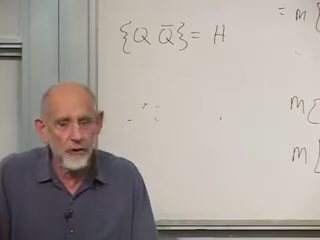
\includegraphics[width=0.62\textwidth]{lecture_05_figure_02.png}
\lectureframe{00:55:46.300}
\caption{La relación de cierre central, aislada en la pizarra. Se ven las llaves y \(Q,\bar Q,H\); la coma queda implícita en la notación habitual del anticonmutador.}
\end{figure}

Se ha elegido el cero aditivo de la energía de modo que el estado vacío tenga \(H=0\). En el oscilador supersimétrico, esta es la convención natural: las contribuciones bosónica y fermiónica de energía de punto cero se cancelan. \editorialnote{La clase trabaja directamente con la energía total en reposo y no muestra por separado los términos de punto cero; la convención indicada explicita esa elección.}

El hamiltoniano es par. También es un generador de simetría: genera traslaciones temporales. Por tanto, los generadores impares no cierran entre sí a menos que se incluya el generador par de traslaciones temporales.

\begin{classroomqa}
\audiencequestion{¿Cuál de los elementos de la relación es par? ¿Es el hamiltoniano? \lecturetimestamp{00:58:24}}
\lecturerresponse{Sí. La energía es un observable ordinario, así que \(H\) es par. La supercarga \(Q\) es impar, y el producto de dos cantidades impares es par; por consiguiente, \(\{Q,\bar Q\}\) puede ser igual a \(H\). Un generador impar y uno par se relacionan mediante un conmutador, no mediante un anticonmutador.}
\end{classroomqa}

\subsection{Completar el álgebra}

Las relaciones entre elementos de igual paridad son inmediatas:
\begin{equation}
\{Q,Q\}=2Q^2=0,
\qquad
\{\bar Q,\bar Q\}=2\bar Q^2=0,
\end{equation}
porque \(Q^2\) contiene \(c_-^2\) y \(\bar Q^2\) contiene \(c_+^2\).

Queda por establecer la relación con \(H\). Sea
\begin{equation}
H\ket{E}=E\ket{E}.
\end{equation}
Si las masas del bosón y del fermión son iguales, \(Q\) transforma uno en el otro sin cambiar la energía. Por tanto, \(Q\ket{E}\) es cero o bien otro estado propio con el mismo autovalor:
\begin{equation}
H Q\ket{E}=E Q\ket{E}.
\end{equation}
Por otro lado,
\begin{equation}
QH\ket{E}=Q(E\ket{E})=E Q\ket{E}.
\end{equation}
Al restar,
\begin{equation}
[H,Q]\ket{E}=0.
\end{equation}
Si los estados propios de la energía forman una base completa, esto vale como identidad de operadores:
\begin{equation}
[H,Q]=0,
\qquad
[H,\bar Q]=0.
\end{equation}

\begin{classroomqa}
\audiencequestion{¿Qué ocurre si el bosón y el fermión no tienen la misma masa? \lecturetimestamp{01:01:16}}
\lecturerresponse{Entonces, al sustituir uno por el otro, cambia la energía, así que la supercarga propuesta no conmuta con el hamiltoniano y se pierde la supersimetría sencilla. Para
\[
H=m_BN_B+m_FN_F,
\]
el resultado explícito es
\[
[H,Q]=(m_B-m_F)Q.
\]
Se anula precisamente cuando \(m_B=m_F\). \editorialnote{El conmutador para masas distintas expresa directamente, en forma de operador, el argumento basado en el cambio de energía y hace explícita la condición de igualdad de masas.}}
\end{classroomqa}

\begin{classroomqa}
\audiencequestion{¿Se puede repetir más despacio el argumento basado en los estados propios de la energía? \lecturetimestamp{01:01:37}}
\lecturerresponse{Partamos de \(H\ket{E}=E\ket{E}\). La igualdad de masas implica que \(Q\ket{E}\) tiene la misma energía definida \(E\), por lo que \(HQ\ket{E}=EQ\ket{E}\). En el otro orden se obtiene \(QH\ket{E}=QE\ket{E}=EQ\ket{E}\), porque \(E\) es un escalar ordinario. Su diferencia se anula en cada estado propio de la energía. La completitud permite extender la afirmación desde esos estados a la ecuación de operadores \([H,Q]=0\).}
\end{classroomqa}

Por tanto, el álgebra completa de este modelo es
\begin{align}
\{Q,\bar Q\}&=H,\\
\{Q,Q\}&=\{\bar Q,\bar Q\}=0,\\
[H,Q]&=[H,\bar Q]=0.
\end{align}
Las supercargas son cargas impares conservadas. Más sorprendentemente, su álgebra combina una operación que cambia el tipo de partícula con el generador de las traslaciones del espacio-tiempo.

\section{Por qué el hamiltoniano representa las traslaciones temporales}

En este modelo simplificado no hay coordenada espacial, pero sí hay tiempo. La ecuación de Schrödinger es
\begin{equation}
i\frac{\partial}{\partial t}\ket{\psi(t)}
=H\ket{\psi(t)}.
\end{equation}

\begin{figure}[H]
\centering
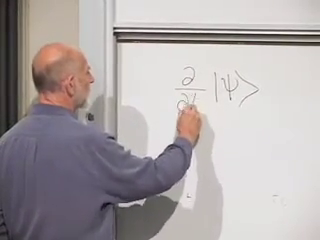
\includegraphics[width=0.56\textwidth]{lecture_05_figure_03.png}
\lectureframe{01:07:26.300}
\caption{La derivada temporal escrita junto a \(\ket{\psi}\). La mano oculta parte del denominador; la ecuación de Schrödinger completa aparece arriba.}
\end{figure}

Para un desplazamiento finito \(\delta\),
\begin{equation}
\ket{\psi(t+\delta)}
=e^{-iH\delta}\ket{\psi(t)}.
\end{equation}
Al desarrollar hasta primer orden,
\begin{equation}
\ket{\psi(t+\delta)}
=\left(\mathbf 1-i\delta H\right)\ket{\psi(t)}
+O(\delta^2).
\end{equation}
Así, \(H\) es el generador infinitesimal que actualiza el estado en el tiempo.

Las simetrías internas, como el isospín y el color, también cambian las etiquetas de las partículas. El isospín puede mezclar los estados del protón y del neutrón; las rotaciones de color mezclan los quarks rojos, verdes y azules. Sin embargo, ninguna composición de esas transformaciones internas traslada un sistema en el espacio o en el tiempo. La supersimetría es distinta:
\begin{equation}
\begin{gathered}
\text{odd particle-changing transformation}\\
\mathrel{\stackrel{\{\ ,\ \}}{\Longrightarrow}}\\
\text{time translation}
\end{gathered}
\end{equation}
Esto indica que los generadores impares podrían ser ellos mismos traslaciones, pero a lo largo de coordenadas distintas de las habituales.

\section{Superspacio}

\subsection{Una función del tiempo y de coordenadas impares}

Introduzcamos una función
\begin{equation}
\Psi=\Psi(\theta,\bar\theta,t).
\end{equation}
Puede interpretarse como una función de onda en el modelo simplificado o, en general, como un supercampo. Como el desarrollo impar se trunca,
\begin{equation}
\Psi(\theta,\bar\theta,t)
=A(t)+\bar\chi(t)\theta
+\bar\theta\chi(t)+F(t)\bar\theta\theta.
\end{equation}
Un único objeto reúne funciones componentes pares e impares. \editorialnote{Este desarrollo en componentes aplica el polinomio de Grassmann introducido antes; constituye el contenido explícito habitual de una función en el superspacio de este modelo.}

Una traslación temporal ordinaria deja fijo \(\theta,\bar\theta\) y transforma
\begin{equation}
t\longmapsto t+\delta.
\end{equation}
A primer orden,
\begin{equation}
\Psi(\theta,\bar\theta,t+\delta)
=\Psi(\theta,\bar\theta,t)
+\delta\,\partial_t\Psi(\theta,\bar\theta,t).
\end{equation}

\begin{figure}[H]
\centering
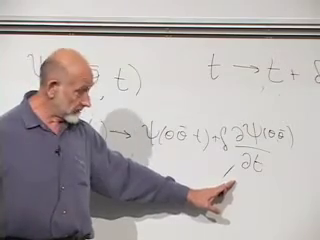
\includegraphics[width=0.72\textwidth]{lecture_05_figure_04.png}
\lectureframe{01:13:15.060}
\caption{La pizarra muestra \(t\to t+\delta\) encima del cambio de primer orden de \(\Psi\), e indica directamente el término de la derivada.}
\end{figure}

\subsection{Traslación en una dirección impar}

Inventemos ahora una transformación que desplace una coordenada impar:
\begin{equation}
\theta\longmapsto\theta+\epsilon,
\end{equation}
donde \(\epsilon\) es otro parámetro impar de Grassmann. Al mismo tiempo, hagamos que el tiempo adquiera un desplazamiento nilpotente par,
\begin{equation}
t\longmapsto t+i\bar\theta\epsilon.
\end{equation}
Tanto \(\bar\theta\) como \(\epsilon\) son impares, así que su producto es par y puede sumarse de manera coherente a la coordenada par \(t\).

Con el parámetro a la izquierda,
\begin{equation}
i\bar\theta\epsilon=-i\epsilon\bar\theta.
\end{equation}
La variación inducida es, por tanto,
\begin{align}
\delta_\epsilon\Psi
&=\epsilon\,\partial_\theta\Psi
-i\epsilon\bar\theta\,\partial_t\Psi\\
&=\epsilon q_0\Psi,
\end{align}
donde
\begin{equation}
q_0=\partial_\theta-i\bar\theta\partial_t.
\end{equation}
Este operador diferencial impar es el generador del desplazamiento combinado. Un generador conjugado compatible, con derivadas izquierdas, es
\begin{equation}
\bar q_0=-\partial_{\bar\theta}
+i\theta\partial_t.
\end{equation}

Los signos exactos dependen de si se usan derivadas izquierdas o derechas de Grassmann y de cómo la conjugación invierte los factores impares. Lo que no debe depender de la convención es el cierre sobre las traslaciones temporales. Con las definiciones anteriores,
\begin{align}
\{q_0,\bar q_0\}
&=i\{\partial_\theta,\theta\}\partial_t
+i\{\bar\theta,\partial_{\bar\theta}\}\partial_t\\
&=2i\partial_t.
\end{align}
El término con dos derivadas se anula, al igual que el término cuadrático en las coordenadas impares. Los dos términos mixtos aportan \(i\partial_t\) cada uno.

Como \(H=i\partial_t\) sobre los estados en la representación de Schrödinger,
\begin{equation}
\{q_0,\bar q_0\}=2H.
\end{equation}
Si normalizamos de modo que
\begin{equation}
q=\frac{q_0}{\sqrt2},
\qquad
\bar q=\frac{\bar q_0}{\sqrt2},
\end{equation}
entonces
\begin{equation}
\boxed{\{q,\bar q\}=H.}
\end{equation}
\editorialnote{La clase desarrolla deliberadamente los signos con cierta incertidumbre y luego observa que aparece un factor de dos. La convención mostrada para las derivadas izquierdas conserva ese cálculo en la pizarra, a la vez que fija una normalización coherente. Otras convenciones habituales trasladan los signos entre los desplazamientos de coordenadas y los generadores.}

\begin{classroomqa}
\audiencequestion{¿De dónde sale el factor final de dos en el anticonmutador del superspacio? \lecturetimestamp{01:24:21}}
\lecturerresponse{Hay dos contribuciones mixtas iguales. Una proviene de \(\{\partial_\theta,\theta\}=1\) y la otra de \(\{\partial_{\bar\theta},\bar\theta\}=1\). Cada una multiplica la derivada temporal. Por eso, para los generadores sin normalizar se obtiene \(2i\partial_t\); un factor \(1/\sqrt2\) en cada supercarga restablece la normalización anterior.}
\end{classroomqa}

\begin{classroomqa}
\audiencequestion{¿Se usó en la construcción la hipótesis de que \(\epsilon\) es pequeño? \lecturetimestamp{01:24:51}}
\lecturerresponse{Se usó la nilpotencia, no una magnitud numérica ordinaria. Como \(\epsilon^2=0\), todo desarrollo en una sola \(\epsilon\) termina tras el primer orden. Llamarla infinitesimal o pequeña es una analogía útil, pero la truncación es exacta.}
\end{classroomqa}

\editorialnote{Los parámetros de Grassmann no tienen una magnitud positiva ordinaria. Su papel como parámetros infinitesimales se debe a la nilpotencia y a la terminación exacta del desarrollo.}

\subsection{El significado geométrico}

El álgebra tiene ahora dos realizaciones equivalentes. En la descripción mediante osciladores, \(Q\) y \(\bar Q\) transforman fermiones en bosones y bosones en fermiones. En la descripción geométrica, \(q\) y \(\bar q\) trasladan una función a través de direcciones impares e inducen un desplazamiento temporal ordinario. En ambas descripciones,
\begin{equation}
\begin{gathered}
\{\text{supercharge},\text{conjugate supercharge}\}\\
=\text{time-translation generator}.
\end{gathered}
\end{equation}

El espacio de coordenadas generalizado que contiene \(t,\theta,\bar\theta\) es el superspacio. En una teoría de campos relativista también contiene las coordenadas espaciales ordinarias, y las supercargas cierran sobre el momento total del espacio-tiempo \(P_\mu\), no solo sobre \(H=P_0\). Curvar esta estructura conduce hacia la supergravedad.

En cierto sentido, las variables de Grassmann son un recurso eficiente para llevar la cuenta de bosones y fermiones. En otro, la relación de cierre expresa algo mucho más profundo: la distinción entre el tipo de partícula y la geometría del espacio-tiempo deja de ser absoluta. Desplazarse dos veces en direcciones impares produce un desplazamiento en una dirección ordinaria. Que la naturaleza realice experimentalmente esta estructura es una cuestión aparte del hecho matemático de que la estructura sea coherente, económica y extraordinariamente rígida.

\chapter{Por qué la supersimetría podría ser importante}

\lectureoverview{Las fluctuaciones del vacío conectan los temas de este capítulo.
Las condiciones de contorno producen la fuerza de Casimir, los efectos de lazos ponen en riesgo la masa del Higgs, nuevas partículas virtuales modifican el comportamiento de los acoplamientos gauge con la escala y la energía del vacío gobierna la expansión cósmica. Estos problemas motivan la supersimetría a baja energía como una forma de estabilizar la escala del Higgs, proporcionar un candidato a materia oscura y mejorar la unificación de los acoplamientos gauge. Después construiremos supercampos usando coordenadas de Grassmann y emplearemos la integración de Berezin para obtener una acción supersimétrica.}

\section{Fluctuaciones del vacío entre placas reflectantes}

Retomamos la supersimetría resolviendo primero una cuestión sobre el efecto Casimir. Coloquemos dos placas reflectantes paralelas separadas una distancia \(d\). Aunque no haya partículas reales, un campo cuántico presenta fluctuaciones del vacío. Podemos imaginarlas como procesos virtuales o, de forma equivalente, como el movimiento de punto cero de los modos oscilatorios del campo. Las placas imponen condiciones de contorno, por lo que las fluctuaciones permitidas entre ellas difieren de las del espacio sin restricciones.

La magnitud importante no es un cero absoluto de energía, sino el cambio que se produce al variar la separación. Denotemos por \(\mathcal E(d)=E(d)/A\) la energía del vacío por unidad de área. Cuando \(\mathcal E\) depende de \(d\), se trata de una energía potencial, y la fuerza por unidad de área es
\begin{equation}
\frac{F}{A}=-\frac{d\mathcal E}{dd}.
\end{equation}
Así, una reorganización de los procesos virtuales se convierte en una fuerza observable. En el conocido ejemplo electromagnético con placas conductoras ideales, la energía y la presión son
\begin{align}
\mathcal E(d)&=-\frac{\pi^2}{720\,d^3},\\
\frac{F}{A}&=-\frac{\pi^2}{240\,d^4},
\end{align}
en unidades \(\hbar=c=1\).\editorialnote{Estos coeficientes y la distinción entre la energía por área \(d^{-3}\) y la presión \(d^{-4}\) resuelven la cuestión dimensional planteada en la pizarra. Son el resultado estándar para placas ideales; aquí no se deriva.} El signo menos indica atracción.

\begin{classroomqa}
\audiencequestion{¿La cuarta potencia describe la fuerza o la energía? \lecturetimestamp{00:04:39}}
\lecturerresponse{Para placas paralelas en cuatro dimensiones del espacio-tiempo, la energía por unidad de área disminuye como \(d^{-3}\), mientras que al derivar respecto de \(d\) la fuerza por unidad de área disminuye como \(d^{-4}\). El análisis dimensional ya determina estas potencias cuando se restituyen \(\hbar\) y \(c\).}
\end{classroomqa}

A veces se resume el cálculo diciendo que las placas interrumpen los lazos virtuales de fotones. Esa imagen es útil siempre que no se tome demasiado literalmente. El cálculo preciso consiste en un cambio del espectro de modos de campo permitidos o, de forma equivalente, un cambio de la acción efectiva cuántica. Ambos lenguajes conducen a la misma energía dependiente de la separación.

\begin{classroomqa}
\audiencequestion{¿Puede la fuerza de Casimir ser repulsiva en lugar de atractiva? \lecturetimestamp{00:07:48}}
\lecturerresponse{Sí. El signo no es universal: depende de los campos, la geometría, los materiales y las condiciones de contorno. Los lazos fermiónicos suelen aportar un signo de lazo opuesto al de los bosónicos, lo que motiva la sugerencia planteada en la pizarra; sin embargo, la estadística fermiónica por sí sola no constituye un teorema general según el cual toda fuerza de Casimir deba ser repulsiva.\editorialnote{Esta precisión sustituye una respuesta deliberadamente tentativa dada en clase por la afirmación general necesaria para evitar una regla universal falsa.}}
\end{classroomqa}

\subsection{¿Qué se consideraría evidencia de la energía del vacío?}

La fuerza de Casimir se mide, y los observables atómicos también son sensibles a los lazos del vacío. Sin embargo, ninguno de estos hechos demuestra por sí solo que la energía absoluta del vacío gravite. Un experimento de Casimir mide una diferencia de energía causada por las condiciones de contorno; es posible describir la misma fuerza sin atribuir significado operativo a una suma ilimitada de energías de punto cero absolutas.

La prueba decisiva viene de la gravedad. La energía es carga gravitatoria. Si el espacio vacío contiene una densidad de energía uniforme, esta debe aparecer en las ecuaciones de Einstein e influir en la expansión cósmica. Por tanto, la expansión acelerada del universo constituye la evidencia gravitatoria directa de un componente similar al vacío.

\begin{classroomqa}
\audiencequestion{¿Por qué los relatos divulgativos llaman misteriosa a la energía del vacío, como si los físicos no supieran qué es? \lecturetimestamp{00:08:19}}
\lecturerresponse{La teoría cuántica de campos asigna una contribución de punto cero a cada campo, así que la posibilidad de que exista energía del vacío no es misteriosa. El misterio es cuantitativo: ¿por qué el valor que gravita es extraordinariamente pequeño en comparación con las estimaciones basadas en los campos cuánticos conocidos y un corte de alta energía? Lo sorprendente es su casi total ausencia, no su mera presencia.}
\end{classroomqa}

Durante muchos años, el límite superior observacional era tan pequeño que resultaba psicológicamente tentador fijar la constante cosmológica exactamente en cero y buscar un principio que impusiera la cancelación. Las mejoras en las observaciones cosmológicas revelaron, en cambio, un valor pequeño pero distinto de cero. Ese descubrimiento no hizo que la energía del vacío resultara conceptualmente ajena; hizo imposible ignorar la magnitud de la supresión que aún no se explica. La comparación pertinente depende de la escala ultravioleta supuesta, pero toda estimación natural de alta energía exige una cancelación enorme.

\section{Qué hace una carga de supersimetría a un estado con muchas partículas}

Antes de enumerar razones para creer en la supersimetría, conviene despejar una posible paradoja. Los bosones pueden ocupar un mismo modo en cantidades arbitrariamente grandes, mientras que la ocupación de un modo fermiónico solo puede ser cero o uno. Si una simetría intercambia bosones y fermiones, ¿convierte mil bosones en un modo en mil fermiones prohibidos?

No. Un generador fermiónico cambia un cuanto cada vez. En el modelo de oscilador, sea \(a\) el operador que aniquila un bosón y \(c^\dagger\) el que crea su compañero fermiónico. Una carga de supersimetría puede representarse como
\begin{equation}
Q=c^\dagger a.
\end{equation}
Sobre un estado con \(n\) bosones y ningún fermión,
\begin{equation}
Q\ket{n,0}
=\sqrt n\,\ket{n-1,1}.
\end{equation}
Se ha eliminado un bosón y se ha insertado un fermión. Si se vuelve a aplicar la misma carga, el resultado es cero:
\begin{equation}
Q^2=(c^\dagger)^2a^2=0.
\end{equation}
Esta es la nilpotencia que se hereda de los operadores de creación fermiónicos.

\begin{classroomqa}
\audiencequestion{Si muchos bosones ocupan el mismo estado, ¿por qué una transformación de supersimetría no produce muchos fermiones en ese mismo estado y viola el principio de exclusión? \lecturetimestamp{00:12:05}}
\lecturerresponse{El generador no sustituye toda la población. Cambia el estado en una unidad de número fermiónico. La misma carga fermiónica no puede acumularse como un generador de rotaciones ordinario, porque su cuadrado se anula. Una carga complementaria puede deshacer el intercambio, y el anticonmutador mixto se cierra en una traslación temporal.}
\end{classroomqa}

La última frase es esencial. La forma abreviada \(Q^2=0\) se aplica a una componente quiral individual o a la carga sencilla que acabamos de escribir; no significa que se anule todo producto de cargas de supersimetría. En supersimetría en cuatro dimensiones,
\begin{equation}
\{Q_\alpha,\bar Q_{\dot\beta}\}
=2\sigma^\mu_{\alpha\dot\beta}P_\mu,
\end{equation}
mientras que
\begin{equation}
\{Q_\alpha,Q_\beta\}=0,
\qquad
\{\bar Q_{\dot\alpha},\bar Q_{\dot\beta}\}=0
\end{equation}
para el álgebra mínima sin cargas centrales.\editorialnote{Esta forma en componentes precisa la abreviatura usada en clase: la acción repetida de la misma carga de supersimetría \(Q\) se anula, mientras que una carga y su conjugada generan una traslación.}

\section{Tres razones para buscar supersimetría a baja energía}

\begin{classroomqa}
\audiencequestion{¿Hay motivos para la supersimetría además de cancelar la energía del vacío? \lecturetimestamp{00:15:06}}
\lecturerresponse{Hay tres motivos estrechamente relacionados: controlar la autoenergía del Higgs, contar con una posible partícula estable de materia oscura y lograr un encuentro mucho más preciso de los acoplamientos gauge a alta energía. Ninguno demuestra que la supersimetría se realice en la naturaleza, pero en conjunto hacen de ella una teoría seria que merece ponerse a prueba.}
\end{classroomqa}

La expresión \emph{supersimetría a baja energía} es relativa. No significa que los supercompañeros sean ligeros en la escala cotidiana, sino que sus masas no están muy por encima de las escalas electrodébil y de los aceleradores. Los tres argumentos se debilitan si las masas de los supercompañeros se elevan arbitrariamente.

\subsection{Proteger la escala del Higgs}

La masa de un escalar es excepcionalmente sensible a la física de alta energía. Esquemáticamente, un lazo bosónico produce una corrección de la forma
\begin{equation}
\delta m_H^2\big|_{\mathrm B}
\sim +\frac{\lambda}{16\pi^2}\Lambda^2,
\end{equation}
donde \(\Lambda\) representa la escala hasta la que se utiliza la teoría efectiva. Un lazo fermiónico lleva el signo opuesto,
\begin{equation}
\delta m_H^2\big|_{\mathrm F}
\sim -\frac{|y|^2}{8\pi^2}\Lambda^2.
\end{equation}
Los coeficientes dependen de la interacción y de las multiplicidades de los campos, pero la supersimetría los relaciona de tal modo que la sensibilidad ultravioleta dominante se cancela entre los supercompañeros.\editorialnote{Las fórmulas esquemáticas de los lazos muestran la matemática que subyace al argumento cualitativo sobre la autoenergía. No pretenden ser un cálculo completo de la masa del Higgs del Modelo Estándar.}

Esto importa porque el valor esperado del Higgs fija la escala electrodébil. Las masas de los bosones gauge y de los fermiones obedecen relaciones como
\begin{equation}
m_W=\frac{gv}{2},
\qquad
m_f=\frac{y_fv}{\sqrt2}.
\end{equation}
Si el sector del Higgs tendiera de forma natural a una escala enorme, se perdería el espectro de partículas conocido a baja energía, a menos que se ajustaran los parámetros desnudos contra las correcciones radiativas con una precisión extrema.

La supersimetría exacta haría exacta la cancelación, pero ya está descartada por las masas desiguales de los bosones y fermiones observados. Con supersimetría rota suavemente, la sensibilidad cuadrática se sustituye por una dependencia de las diferencias de masa entre supercompañeros, esquemáticamente
\begin{equation}
\delta m_H^2
\sim
\frac{g^2}{16\pi^2}
\left(m_{\mathrm{soft}}^2-m_{\mathrm{ordinary}}^2\right)
\ln\frac{\Lambda^2}{m_{\mathrm{soft}}^2}.
\end{equation}
La cancelación solo resulta útil mientras la diferencia de masas no sea demasiado grande.

\subsection{Un estado final estable para las cascadas de materia oscura}

Dividamos el espectro entre partículas ordinarias y sus supercompañeros. Un fermión tiene un supercompañero bosónico; un bosón, uno fermiónico. Si las interacciones conservan una paridad que distingue estas dos clases, la desintegración de un supercompañero debe dejar otro supercompañero:
\begin{equation}
\widetilde X
\longrightarrow X+\widetilde Y
\longrightarrow X+Y+\widetilde Z
\longrightarrow\cdots.
\end{equation}
La cascada no puede descartar su último supercompañero. Por tanto, termina en la partícula supersimétrica más ligera, el LSP.

La simetría que se usa habitualmente es la paridad \(R\),
\begin{equation}
R_p=(-1)^{3(B-L)+2s}.
\end{equation}
Las partículas del Modelo Estándar tienen \(R_p=+1\), mientras que sus supercompañeros tienen \(R_p=-1\). Si \(R_p\) es exacta, toda interacción contiene un número par de supercompañeros y el LSP es estable.\editorialnote{La supersimetría por sí sola no garantiza que el LSP sea estable. La estabilidad requiere que se conserve la paridad \(R\) u otra simetría con la misma consecuencia; sin ella, el LSP puede desintegrarse.}

La materia oscura debe sobrevivir al menos durante escalas de tiempo cosmológicas. También debe interactuar con suficiente debilidad como para atravesar repetidamente el disco galáctico visible sin perder una cantidad sustancial de energía. Una población con carga eléctrica o interacciones fuertes dispersaría, disiparía energía y tendería a colapsar hasta formar la misma estructura delgada que la materia ordinaria. El halo extendido observado apunta, en cambio, a un componente neutro y débilmente interactuante.

Esto no identifica de manera única al LSP. Según el modelo y el patrón de ruptura de la simetría, el candidato podría ser una mezcla neutra de gauginos electrodébiles e higgsinos, o bien un gravitino. Los candidatos cargados o coloreados están fuertemente restringidos. Lo que aporta la supersimetría no es una respuesta garantizada, sino un mecanismo natural para producir un estado final neutro y longevo.

\section{Acoplamientos variables con la escala y el indicio de unificación}

El tercer motivo parte del apantallamiento de la carga. Un acoplamiento medido depende de la escala de energía porque las partículas virtuales modifican la interacción. En el electromagnetismo, un lazo electrón-positrón insertado en un propagador del fotón apantalla la carga a larga distancia. A distancias menores, o con mayor transferencia de momento, queda menos nube de polarización entre las partículas de prueba y la carga efectiva es mayor.

Escribamos
\begin{equation}
\alpha_i=\frac{g_i^2}{4\pi}.
\end{equation}
A un lazo, el inverso del acoplamiento varía linealmente con el logaritmo de la energía:
\begin{equation}
\frac{d\alpha_i^{-1}}{d\ln\mu}
=-\frac{b_i}{2\pi}.
\end{equation}
Así,
\begin{equation}
\alpha_i^{-1}(\mu)
=\alpha_i^{-1}(\mu_0)
-\frac{b_i}{2\pi}\ln\frac{\mu}{\mu_0}.
\end{equation}
\editorialnote{Esta ecuación a un lazo es la formulación precisa de las rectas casi perfectas que se dibujan en función del logaritmo de la energía. Los umbrales y las correcciones de órdenes superiores curvan ligeramente las líneas.}

Por encima de la escala electrodébil, los tres acoplamientos gauge fundamentales corresponden a
\begin{equation}
U(1)_Y,\qquad SU(2)_L,\qquad SU(3)_c.
\end{equation}
El acoplamiento electromagnético que se emplea para orientarse a baja energía es una combinación de los dos primeros tras la ruptura de la simetría electrodébil. En QCD, los campos gauge no abelianos producen antiapantallamiento: el acoplamiento fuerte disminuye a distancias cortas, fenómeno conocido como libertad asintótica. Por consiguiente, \(\alpha_3^{-1}\) aumenta con \(\ln\mu\), mientras que los inversos de los otros acoplamientos tienen pendientes distintas.

Las curvas del Modelo Estándar apuntan sugestivamente unas hacia otras, pero no se cruzan en un único punto. Los supercompañeros modifican los lazos virtuales y, por tanto, cambian los coeficientes \(b_i\). En la normalización convencional de gran unificación,
\begin{align}
(b_1,b_2,b_3)_{\mathrm{SM}}
&=\left(\frac{41}{10},-\frac{19}{6},-7\right),\\
(b_1,b_2,b_3)_{\mathrm{MSSM}}
&=\left(\frac{33}{5},1,-3\right).
\end{align}
Con umbrales de los supercompañeros cerca de la escala del TeV, las curvas supersimétricas extrapoladas se encuentran con mucha más precisión cerca de
\begin{equation}
M_{\mathrm{GUT}}\sim 10^{16}\ \mathrm{GeV}.
\end{equation}
Ningún experimento alcanza directamente esa escala. Se miden los acoplamientos a baja energía, el contenido de campos determina su evolución con la escala y las curvas se extrapolan a lo largo de muchas décadas. Dos líneas siempre se cruzan en algún punto; que tres líneas independientes se encuentren cerca de un mismo punto es la observación no trivial.

\begin{classroomqa}
\audiencequestion{¿La extrapolación mejorada supone supersimetría exacta y masas iguales para los supercompañeros? \lecturetimestamp{00:38:09}}
\lecturerresponse{No. La supersimetría está rota, así que las masas son distintas. Lo que importa es cuándo empiezan a contribuir los lazos de los supercompañeros a la evolución de los acoplamientos. Si no son demasiado pesados, las pendientes cambian con suficiente antelación para que converjan los tres acoplamientos. Si son extremadamente pesados, los umbrales supersimétricos aparecen demasiado tarde y se pierde el encuentro más preciso.}
\end{classroomqa}

Las correcciones de umbral y el espectro desconocido de alta energía impiden afirmar literalmente que las tres líneas se encuentran con exactitud matemática. Aun así, el resultado es sorprendente: la misma escala aproximada de los supercompañeros que ayuda con el Higgs y proporciona un candidato a materia oscura térmica también mejora la unificación.

\subsection{La gravedad y la escala común de alta energía}

La gravedad se comporta de otra manera porque su carga es la propia energía. Una medida adimensional útil a una energía del centro de masas \(E\) es
\begin{equation}
\alpha_G(E)\sim GE^2
=\left(\frac{E}{M_{\mathrm{Pl}}}\right)^2.
\end{equation}
A energías ordinarias es extraordinariamente pequeña, pero crece cuadráticamente con \(E\). Por eso, su inversa disminuye mucho más rápido que los inversos de los acoplamientos gauge, que varían logarítmicamente, y se vuelve del orden de la unidad cerca de la escala de Planck.

Esta comparación sugiere que todas las interacciones podrían estar regidas por escalas altas cercanas entre sí, pero es menos clara que la unificación gauge. Los acoplamientos gauge son parámetros adimensionales en teorías de campos renormalizables; la constante de Newton tiene dimensiones, por lo que representar la gravedad en la misma gráfica requiere adoptar una convención.

\begin{classroomqa}
\audiencequestion{¿Los supercompañeros participan en las mismas tres interacciones gauge o definen fuerzas nuevas? \lecturetimestamp{00:42:35}}
\lecturerresponse{Tienen los mismos números cuánticos gauge que sus compañeros. Un selectrón tiene la carga eléctrica del electrón, y un escuark tiene el color y las cargas electrodébiles correspondientes a las del quark, aunque sus espines y masas sean distintos. Por tanto, sus lazos modifican las mismas interacciones gauge, en lugar de introducir tres interacciones nuevas.}
\end{classroomqa}

\begin{classroomqa}
\audiencequestion{¿El descubrimiento de un supercompañero en el LHC sería una prueba definitiva de la supersimetría? \lecturetimestamp{00:43:27}}
\lecturerresponse{Una sola partícula desconocida no bastaría por el mero hecho de llevar ese nombre, pero un espectro de supercompañeros que obedeciera las relaciones supersimétricas entre espines, cargas, masas y acoplamientos sería muy distintivo. La supersimetría impone muchas restricciones correlacionadas, por lo que el patrón detallado de interacciones proporcionaría la prueba decisiva.}
\end{classroomqa}

\subsection{Por qué no se puede desplazar la escala sin pagar un precio}

Si los supercompañeros están apenas más allá del alcance experimental, los tres motivos aún pueden ser válidos. Si sus masas aumentan varios órdenes de magnitud, cada argumento pierde fuerza:
\begin{enumerate}\item Las cancelaciones de la masa del Higgs dejan una gran sensibilidad residual a la diferencia de masas.
\item Ya no aparece una reliquia térmica convencional de escala electrodébil en la escala esperada.
\item Los umbrales de la evolución de los acoplamientos se desplazan hacia arriba y los tres acoplamientos se encuentran con menor precisión.
\end{enumerate}
La supersimetría aún podría existir a una escala mucho mayor, pero ya no resolvería estos problemas concretos de baja energía con la misma economía. La longevidad de la idea no demuestra que la naturaleza tenga que emplearla; demuestra que la propuesta es coherente y merece una prueba decisiva.

\section{Qué puede y qué no puede decirnos la cosmología sobre la materia oscura}

\begin{classroomqa}
\audiencequestion{¿Puede la cosmología estándar determinar la cantidad de materia oscura y la masa de cada partícula de materia oscura, del mismo modo que la nucleosíntesis permite restringir las cantidades de hidrógeno y helio? \lecturetimestamp{00:46:32}}
\lecturerresponse{La cosmología mide muy bien la densidad total de masa de materia oscura, pero la densidad por sí sola no permite separar la masa del número de partículas. La misma densidad podría corresponder a unas pocas partículas pesadas o a un número enorme de partículas muy ligeras. Para identificar la partícula microscópica hace falta teoría adicional u observaciones no gravitatorias.}
\end{classroomqa}

Dos posibilidades generales ilustran esta ambigüedad. Una partícula débilmente interactuante, cercana a la escala electrodébil o del TeV, puede desacoplarse térmicamente de un baño caliente. En el extremo opuesto, un bosón extremadamente ligero, como el axión, puede ocupar una configuración de campo coherente o un condensado. Las posibilidades intermedias no quedan descartadas solo porque los dos mecanismos mejor desarrollados se encuentren cerca de extremos opuestos.

La propia estructura del halo impone una restricción importante. La materia oscura atraviesa la materia ordinaria con poca fricción, por lo que permanece extendida espacialmente en lugar de colapsar en el disco luminoso. Las curvas de rotación y otros fenómenos gravitatorios nos indican que la masa está presente, pero no permiten contar las partículas por sí solos.

\begin{classroomqa}
\audiencequestion{¿Es posible que el universo primitivo contuviera inicialmente solo superpartículas, que luego se desintegraran en las partículas que observamos? \lecturetimestamp{00:49:11}}
\lecturerresponse{A temperaturas mucho mayores que todas las masas pertinentes, las reacciones rápidas llevan las especies al equilibrio térmico, en lugar de mantener una población unilateral arbitraria. Las colisiones ordinarias crean supercompañeros cuando estos escasean, mientras que las colisiones y desintegraciones de supercompañeros reponen las partículas ordinarias. La abundancia precisa depende de las interacciones y de los grados de libertad, pero el plasma caliente tiende continuamente al equilibrio.}
\end{classroomqa}

A medida que el universo se enfría, las especies masivas quedan suprimidas por el factor de Boltzmann y se aniquilan o desintegran. Un LSP estable deja de seguir el equilibrio cuando su tasa de interacción se vuelve más lenta que la expansión cósmica:
\begin{equation}
\Gamma_{\mathrm{ann}}
\sim n\langle\sigma v\rangle
\lesssim H.
\end{equation}
Las partículas restantes constituyen una abundancia relicta.\editorialnote{Este criterio de desacoplamiento completa de forma cuantitativa el argumento del equilibrio térmico. Otros candidatos a LSP, en especial los gravitinos con acoplamiento muy débil, pueden tener historias no térmicas.}

\begin{classroomqa}
\audiencequestion{¿De qué partícula ordinaria es supercompañero el LSP, y debe carecer de interacciones? \lecturetimestamp{00:51:05}}
\lecturerresponse{No hay una respuesta independiente del modelo. Se espera que un LSP viable como materia oscura sea eléctricamente neutro y no tenga color, pero no tiene por qué carecer por completo de interacciones. Puede ser una mezcla relacionada con el fotón, los bosones gauge débiles y los campos del Higgs, o puede ser el gravitino. Su identidad precisa se deduce del espectro de ruptura de la supersimetría.}
\end{classroomqa}

\section{Diagramas del vacío, diagramas de autoenergía y expansión}

\begin{classroomqa}
\audiencequestion{¿Cuál es la diferencia entre la divergencia del Higgs y la divergencia de la energía del vacío? \lecturetimestamp{00:52:09}}
\lecturerresponse{Un diagrama del vacío no tiene líneas externas de partículas; modifica la acción efectiva del espacio vacío y contribuye a la energía del vacío. Un diagrama de autoenergía del Higgs tiene dos líneas externas del Higgs; modifica el propagador del Higgs y, por tanto, su masa. Ambos implican fluctuaciones virtuales, pero responden a preguntas distintas.}
\end{classroomqa}

Podemos imaginar una partícula real como una impureza insertada en el vacío. Las fluctuaciones del vacío que se acoplan a ella modifican su propagación y su masa. Las placas de Casimir también modifican las fluctuaciones del vacío, pero mediante condiciones de contorno macroscópicas. En todos los casos, el elemento común es la respuesta de las fluctuaciones cuánticas a algo que se ha introducido; lo que difiere es el observable cuya corrección se calcula.

\vspace{-2pt}
\subsection{La materia, la radiación y el vacío se diluyen de maneras distintas}

Sea \(a(t)\) el factor de escala cosmológico y
\begin{equation}
H=\frac{\dot a}{a}
\end{equation}
el parámetro de Hubble. La conservación local del tensor de energía-momento en un universo homogéneo da
\begin{equation}
\dot\rho+3H(\rho+p)=0.
\end{equation}
Para una ecuación de estado \(p=w\rho\), esto se integra y da
\begin{equation}
\rho(a)\propto a^{-3(1+w)}.
\end{equation}
\editorialnote{La ecuación de continuidad proporciona la derivación concisa que sustenta las explicaciones basadas en el recuento de partículas y el estiramiento de las longitudes de onda.}

Para la materia fría no relativista, \(p\approx0\), así que
\begin{equation}
\rho_m\propto a^{-3}.
\end{equation}
Un volumen comóvil fijo crece como \(a^3\), mientras que la energía en reposo transportada por sus partículas permanece aproximadamente constante.

Para la radiación, \(p=\rho/3\), y
\begin{equation}
\rho_r\propto a^{-4}.
\end{equation}
Tres potencias proceden de la dilución de la densidad numérica. La cuarta se debe al corrimiento al rojo:
\begin{equation}
\lambda\propto a,
\qquad
E_\gamma=\frac{2\pi\hbar c}{\lambda}\propto a^{-1}.
\end{equation}

\begin{classroomqa}
\audiencequestion{Si un fotón tiene una función de onda, ¿por qué podemos hablar de él como partícula y no como onda al derivar la ley de dilución? \lecturetimestamp{00:58:21}}
\lecturerresponse{La distinción no afecta a la dependencia con la escala. En la descripción de partículas, el número de cuantos en un volumen comóvil permanece fijo y cada cuanto experimenta un corrimiento al rojo como \(a^{-1}\). En la descripción de ondas clásicas, la longitud de onda se estira y la energía del campo disminuye en la misma proporción. Podemos usar el lenguaje que haga más fácil visualizar la expansión.}
\end{classroomqa}

La energía del vacío tiene \(p_\Lambda=-\rho_\Lambda\), así que
\begin{equation}
\rho_\Lambda=\text{constant}.
\end{equation}
No se diluye al expandirse el espacio. De hecho, una región comóvil contiene
\begin{equation}
E_\Lambda=\rho_\Lambda a^3V_0,
\end{equation}
que crece con su volumen físico. Este hecho plantea la cuestión de la conservación de la energía que abordaremos en breve.

Las distintas potencias organizan la historia cósmica. La radiación disminuye más deprisa, la materia disminuye más lentamente y la energía del vacío no disminuye en absoluto. Por tanto, un término de vacío diminuto puede ser insignificante en el universo temprano y dominar en épocas tardías. Según los valores aproximados comentados aquí, el presupuesto energético actual consta de aproximadamente \(70\%\) de energía del vacío y \(30\%\) de materia, con una contribución de radiación mucho menor.

\section{La geometría es igual a la energía}

La componente tiempo-tiempo de las ecuaciones de Einstein convierte las leyes de escala anteriores en dinámica. La pizarra empieza con un lema y un único término geométrico.

\begin{figure}[H]
\centering
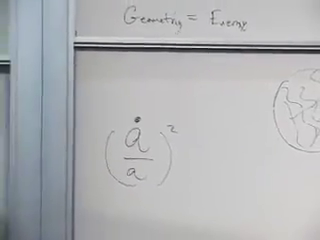
\includegraphics[width=0.68\textwidth]{lecture_06_figure_03.png}
\lectureframe{01:06:37.088}
\caption{El lema organizador \emph{la geometría es igual a la energía}, con el término de expansión \(H^2=(\dot a/a)^2\) escrito debajo.}
\end{figure}

Para un universo homogéneo e isótropo, la primera ecuación de Friedmann es
\begin{equation}
H^2+\frac{k}{a^2}
=\frac{8\pi G}{3}\rho,
\end{equation}
en unidades \(c=1\), donde \(k=+1,0,-1\) denota una geometría espacial cerrada, plana o abierta, y
\begin{equation}
\rho
=\rho_{\mathrm{ordinary}}
+\rho_{\mathrm{dark}}
+\rho_{\mathrm{radiation}}
+\rho_{\mathrm{vacuum}}.
\end{equation}
El signo que aparece junto a \(1/a^2\) depende de si el término de curvatura se deja a la izquierda o se pasa a la derecha, así como del valor de \(k\).

\begin{figure}[H]
\centering
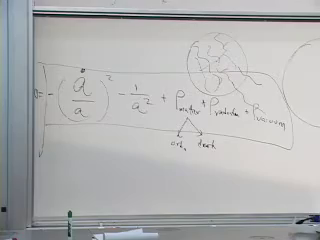
\includegraphics[width=0.96\textwidth]{lecture_06_figure_04.png}
\lectureframe{01:08:46.794}
\caption{El balance completo de la pizarra: expansión y curvatura espacial en el lado geométrico, y materia, radiación y energía del vacío en el lado de las fuentes. La materia se desglosa además en componentes ordinaria y oscura.}
\end{figure}

\subsection{La restricción hamiltoniana cosmológica}

\begin{classroomqa}
\audiencequestion{Si la energía del vacío en una región comóvil crece al expandirse el universo, ¿hay una densidad de energía neta constante o una energía total conservada? \lecturetimestamp{01:01:51}}
\lecturerresponse{La relatividad general no proporciona una energía global universal para un espacio-tiempo expansivo arbitrario. Sin embargo, en la reducción cosmológica homogénea, la ecuación de Einstein tiempo-tiempo es una restricción hamiltoniana. Cuando se colocan la geometría y la materia en un mismo lado, el hamiltoniano restringido se anula. Los términos de materia variables quedan compensados por los grados de libertad gravitatorios, y no por una energía ordinaria fija dentro de una caja.}
\end{classroomqa}

Esquemáticamente, la formulación canónica es
\begin{equation}
\mathcal H_{\mathrm{gravity}}
+\mathcal H_{\mathrm{matter}}
=0.
\end{equation}
Este es el significado preciso de afirmar que la energía total es cero. Se trata de una ecuación de movimiento impuesta por la invariancia ante reparametrizaciones temporales, no de afirmar que toda densidad de energía local se anule. En un volumen comóvil, la energía de la materia ordinaria se mantiene aproximadamente constante, la energía de la radiación disminuye y la energía del vacío aumenta; mientras tanto, la contribución gravitatoria y la tasa de expansión se ajustan para que la restricción de Einstein siga satisfaciéndose.

La conservación local sigue siendo exacta:
\begin{equation}
\nabla_\mu T^{\mu\nu}=0.
\end{equation}
Para el fluido homogéneo, esta es precisamente la ecuación de continuidad
\(\dot\rho+3H(\rho+p)=0\). Lo que en general deja de cumplirse es la intuición propia del espacio-tiempo plano de que también debe existir una única suma global de la energía de la materia, independiente de las coordenadas, que se conserve en un universo en expansión.\editorialnote{Esta distinción precisa la afirmación didáctica de que la energía siempre es cero: la conservación covariante local y la restricción hamiltoniana cosmológica son exactas, mientras que, en general, no está definida una energía global única de materia más gravedad.}

\begin{classroomqa}
\audiencequestion{¿Es la restricción de energía nula la condición que determina si el universo es abierto, cerrado o plano? \lecturetimestamp{01:04:42}}
\lecturerresponse{No. La restricción hamiltoniana se aplica en todos los casos. Los universos abiertos, planos y cerrados se distinguen por el parámetro de curvatura \(k\) y, por tanto, por el término \(k/a^2\). La curvatura modifica una contribución al balance; no activa ni desactiva la restricción.}
\end{classroomqa}

\section{Coordenadas de Grassmann y supercampos}

\begin{classroomqa}
\audiencequestion{¿Aparecen realmente los números de Grassmann en el lagrangiano de la teoría? \lecturetimestamp{01:09:37}}
\lecturerresponse{Aparecen primero porque los campos fermiónicos son impares de Grassmann. Aparecen una segunda vez como coordenadas del espacio supersimétrico. Los supercampos dependen de esas coordenadas impares, y las acciones supersimétricas se construyen derivando e integrando con respecto a ellas.}
\end{classroomqa}

Un campo ordinario es una función del espacio-tiempo,
\begin{equation}
\phi=\phi(x^\mu).
\end{equation}
La supersimetría mínima en cuatro dimensiones amplía \(x^\mu\) con un espinor impar de dos componentes \(\theta^\alpha\) y su conjugado \(\bar\theta^{\dot\alpha}\):
\begin{equation}
z^M=(x^\mu,\theta^\alpha,\bar\theta^{\dot\alpha}).
\end{equation}
Hay dos componentes impares complejas, o cuatro direcciones impares reales. Un supercampo es una función definida en este espacio supersimétrico:
\begin{equation}
\Phi=\Phi(x,\theta,\bar\theta).
\end{equation}

Estas no son dimensiones espaciales diminutas en el sentido métrico. Una coordenada de Grassmann no tiene una magnitud numérica positiva. Llamarla pequeña es una regla mnemotécnica para recordar la nilpotencia:
\begin{equation}
(\theta^\alpha)^2=0,
\qquad
\theta^\alpha\theta^\beta=-\theta^\beta\theta^\alpha.
\end{equation}
\editorialnote{La razón por la que toda expansión en un número finito de coordenadas de Grassmann termina es la nilpotencia, no la pequeñez numérica.}

Con cuatro coordenadas impares independientes, un supercampo completamente general tiene como máximo \(2^4=16\) monomios de Grassmann. Esquemáticamente,
\begin{equation}
\begin{aligned}
\Phi(x,\Theta)={}&\phi(x)+\Theta_A\psi_A(x)\\
&+\frac{1}{2}\Theta_A\Theta_B Z_{AB}(x)+\cdots\\
&+\Theta_1\Theta_2\Theta_3\Theta_4D(x),
\end{aligned}
\end{equation}
donde \(\Theta_A\) representa colectivamente las cuatro coordenadas impares reales. Como se puede elegir que el supercampo completo sea par, los coeficientes de las potencias pares son bosónicos y los de las potencias impares son fermiónicos. Así, un supercampo reúne un multiplete finito de campos componentes ordinarios.

Esta forma de agruparlos es más que una notación. La supersimetría actúa geométricamente como una traslación en las direcciones impares, combinada con una traslación en el espacio-tiempo. Un lagrangiano construido a partir de supercampos según las reglas del espacio supersimétrico hereda la simetría, del mismo modo que un lagrangiano escalar construido a partir de tensores hereda la invariancia rotacional o de Lorentz.

La acción incluye ahora medidas de Grassmann. Un término típico de espacio supersimétrico completo tiene la forma
\begin{equation}
S_D=\int d^4x\,d^2\theta\,d^2\bar\theta\,
\mathcal K(\Phi,\Phi^\dagger).
\end{equation}
Los términos quirales usan, en cambio,
\begin{equation}
S_F=\int d^4x\,d^2\theta\,W(\Phi)+\mathrm{h.c.}
\end{equation}
\editorialnote{La distinción entre medidas de espacio supersimétrico completo y medidas quirales es el refinamiento estándar de la acción esquemática \(d^4x\,d^4\theta\). Los ejemplos concretos determinarán qué medida corresponde utilizar.}

Hemos llegado, por tanto, a una pregunta que el cálculo ordinario no responde: ¿qué significa integrar respecto de una coordenada anticonmutativa?

\section{Integración de Berezin}

\subsection{El modelo ordinario: una derivada total}

Comencemos con una función ordinaria \(F(x)\) que se anula cuando \(x\) tiende a valores positivos y negativos grandes. El teorema fundamental del cálculo da
\begin{equation}
\int_{-\infty}^{\infty}dx\,\frac{dF}{dx}
=F(\infty)-F(-\infty)
=0.
\end{equation}

\begin{figure}[H]
\centering
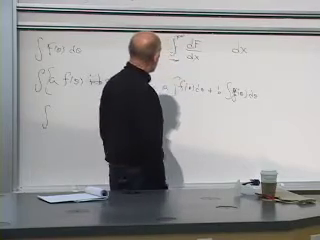
\includegraphics[width=0.88\textwidth]{lecture_06_figure_05.png}
\lectureframe{01:26:31.594}
\caption{El modelo ordinario de la integración de Berezin: la integral de una derivada total se reduce a los valores en los extremos y se anula cuando la función tiende a cero. La línea inferior de la pizarra está parcialmente tapada, así que el texto presenta la ecuación sin obstrucciones.}
\end{figure}

Queremos que la integral de Grassmann sea lineal y comparta la propiedad útil de que la integral de una derivada total se anule. Para una coordenada impar, exigimos
\begin{align}
\int d\theta\,[af(\theta)+bg(\theta)]
&=
a\int d\theta\,f(\theta)
+b\int d\theta\,g(\theta),\\
\int d\theta\,\partial_\theta f(\theta)&=0.
\end{align}
La segunda condición es el análogo algebraico de la invariancia de la medida ante traslaciones. No hay extremos de una recta numérica impar ni una suma sobre intervalos diminutos.

\begin{classroomqa}
\audiencequestion{Si no existe una integral indefinida de Grassmann, ¿estamos abandonando la idea de que integrar es la operación inversa de derivar? \lecturetimestamp{01:21:19}}
\lecturerresponse{Sí. La integración de Berezin es un funcional lineal definido, no una operación de hallar primitivas. De hecho, para una variable de Grassmann, está representada por la misma operación algebraica que la derivación.}
\end{classroomqa}

\begin{classroomqa}
\audiencequestion{¿La integración respecto de \(d^4x\) todo el espacio-tiempo también es una integral definida? \lecturetimestamp{01:21:34}}
\lecturerresponse{Sí. Al integrar la acción sobre el espacio-tiempo se sobreentienden las condiciones de contorno. La diferencia es que la integración ordinaria sobre el espacio-tiempo puede entenderse mediante límites de sumas, mientras que la integración de Grassmann se define algebraicamente por su acción sobre la base finita \(1,\theta\).}
\end{classroomqa}

\subsection{Una variable}

Toda función de una variable impar se puede escribir con su coeficiente en el orden fijo, a la derecha:
\begin{equation}
f(\theta)=a+\theta b.
\end{equation}
Como \(\partial_\theta\theta=1\), la regla para las derivadas totales implica
\begin{equation}
\int d\theta\,1=0.
\end{equation}
La normalización restante se elige como
\begin{equation}
\int d\theta\,\theta=1.
\end{equation}
Por consiguiente,
\begin{equation}
\int d\theta\,f(\theta)=b.
\end{equation}
La integral selecciona el coeficiente de la potencia más alta disponible. Con la convención de derivada por la izquierda usada aquí,
\begin{equation}
\partial_\theta f=b
=\int d\theta\,f.
\end{equation}

\begin{classroomqa}
\audiencequestion{¿Existe una función \(F(\theta)\) que satisfaga \(\partial_\theta F=\theta\)? \lecturetimestamp{01:30:05}}
\lecturerresponse{No. Tal función tendría que incluir un término proporcional a \(\theta^2\), pero \(\theta^2=0\). Esta es otra manera de ver por qué no existe un análogo de una primitiva indefinida para las variables de Grassmann.}
\end{classroomqa}

\subsection{Dos variables y el orden de la medida}

Para un par complejo \(\theta,\bar\theta\), escribamos una función general par en la forma ordenada
\begin{equation}
f(\theta,\bar\theta)
=a+\bar\theta\psi+\bar\psi\theta+b\,\bar\theta\theta.
\end{equation}
No hay términos de orden superior porque
\begin{equation}
\theta^2=\bar\theta^2=0,
\qquad
\bar\theta\theta=-\theta\bar\theta.
\end{equation}

Fijamos ahora la convención
\begin{equation}
\int d\theta\,d\bar\theta\,
\bar\theta\theta=1.
\end{equation}
En las integrales iteradas, la operación adyacente \(d\bar\theta\) actúa primero. La tabla queda entonces
\begin{align}
\int d\theta\,d\bar\theta\,1&=0,\\
\int d\theta\,d\bar\theta\,\theta&=0,\\
\int d\theta\,d\bar\theta\,\bar\theta&=0,\\
\int d\theta\,d\bar\theta\,\bar\theta\theta&=1.
\end{align}
Por tanto,
\begin{equation}
\int d\theta\,d\bar\theta\,
f(\theta,\bar\theta)=b.
\end{equation}

\begin{classroomqa}
\audiencequestion{Para un término lineal en \(\theta\), ¿es realmente la integración respecto de \(\theta\) la que hace que la integral doble se anule? \lecturetimestamp{01:34:59}}
\lecturerresponse{No; la explicación oral invirtió los papeles. Integrar \(\theta\) con respecto a \(\theta\) da uno. El resultado ya no contiene \(\bar\theta\), y la integral restante de uno respecto de \(\bar\theta\) se anula. En cualquier caso, la integral doble solo es distinta de cero cuando aparecen ambas variables.}
\end{classroomqa}

\begin{classroomqa}
\audiencequestion{Si se intercambian \(\theta\) y \(\bar\theta\), ¿cambia de signo la integral? \lecturetimestamp{01:36:33}}
\lecturerresponse{Sí. Las variables impares y las medidas impares anticonmutan. Con la convención anterior,
\[
\int d\bar\theta\,d\theta\,\bar\theta\theta=-1.
\]
Por tanto, hay que elegir un orden y mantenerlo de manera coherente. La física es independiente de la convención, pero los signos intermedios no lo son.}
\end{classroomqa}

Para \(n\) variables de Grassmann independientes, el patrón es inmediato:
\begin{equation}
\int d\theta_n\cdots d\theta_1\,
f(\theta_1,\ldots,\theta_n)
\end{equation}
extrae el coeficiente del monomio de grado máximo ordenado
\(\theta_1\cdots\theta_n\), con el signo determinado por el orden elegido para las variables y las medidas. Esta sencilla regla de extracción de componentes es la clave de las acciones en el espacio supersimétrico. Una variación supersimétrica se convierte en una derivada total impar, y la integral en el espacio supersimétrico la elimina, del mismo modo que una acción ordinaria elimina una derivada total en el espacio-tiempo bajo condiciones de contorno adecuadas.

\section{Por qué un cálculo tan sencillo tiene tanta potencia}

Las reglas parecen casi triviales:
\begin{equation}
\int d\theta\,1=0,
\qquad
\int d\theta\,\theta=1.
\end{equation}
Sin embargo, nos permiten construir teorías de campos con interacciones en las que las relaciones entre las masas y los acoplamientos bosónicos y fermiónicos se conservan automáticamente. El propósito del cálculo en el espacio supersimétrico es el mismo que el del cálculo tensorial en relatividad: organizar la notación de modo que la simetría deseada se conserve en todas las manipulaciones permitidas.

Llevar la cuenta de los signos es el precio. Cada intercambio de dos objetos impares aporta un signo menos, y un cálculo puede ser conceptualmente correcto y, aun así, fallar por una elección equivocada del orden. Esta dificultad no es decorativa: es la manifestación algebraica de la estadística fermiónica.

\begin{classroomqa}
\audiencequestion{¿Se inventaron los números de Grassmann junto con la supersimetría o ya existían antes? \lecturetimestamp{01:41:19}}
\lecturerresponse{Son mucho más antiguos. Hermann Grassmann desarrolló el álgebra exterior subyacente en el siglo XIX. Las formas diferenciales ya usan elementos de base anticonmutativos; la teoría cuántica de campos y la supersimetría del siglo XX encontraron un nuevo papel físico para las mismas matemáticas.}
\end{classroomqa}

Ya estamos preparados para realizar construcciones concretas. Los supercampos reúnen multipletes completos de bosones y fermiones, las derivadas en el espacio supersimétrico preservan el álgebra y la integración de Berezin extrae la acción en términos de componentes. La tarea siguiente consiste en emplear estas herramientas en el modelo unidimensional más sencillo y luego extenderlas a la teoría de campos.

\chapter{El supersespacio y la construcción de la dinámica supersimétrica}

\lectureoverview{Reconstruimos la supersimetría a partir del sistema más pequeño en el que puede actuar: un oscilador bosónico y otro fermiónico con la misma energía. El contraste entre sus ecuaciones de segundo y primer orden conduce a las cargas supersimétricas y a su álgebra. Después reinterpretamos esa álgebra como geometría en un espacio con la coordenada ordinaria (t) y las coordenadas de Grassmann \(\theta,\bar\theta\). Los supercampos reúnen los bosones, los fermiones y un campo auxiliar en un solo objeto; la integración de Berezin extrae un lagrangiano ordinario invariante; las derivadas covariantes permiten imponer restricciones compatibles con la simetría; y la restricción quiral ofrece el primer ejemplo importante. La lección muestra deliberadamente las dificultades de signos y ordenación de este formalismo y concluye explicando por qué la simetría misma es más fundamental que un catálogo de reglas de Feynman.}

\section{Volvamos al sistema de un modo}

Empecemos de nuevo con fermiones y bosones en reposo. Omitimos todas las coordenadas espaciales y las etiquetas de momento. En un modo dado, un cuanto está presente o ausente, y basta con los operadores de creación y aniquilación para describirlo. Escribamos \(a^\dagger,a\) para un modo bosónico y \(c^\dagger,c\) para uno fermiónico. Satisfacen
\begin{align}
[a,a^\dagger]&=1,
&
\{c,c^\dagger\}&=1,
&
c^2=(c^\dagger)^2&=0.
\end{align}
Si ambos cuantos tienen la misma energía \(m\), entonces, salvo una constante irrelevante del vacío,
\begin{equation}
H=m\left(a^\dagger a+c^\dagger c\right).
\label{eq:l7-one-mode-hamiltonian}
\end{equation}
El operador número \(a^\dagger a\) puede tomar cualquier valor entero no negativo, mientras que \(c^\dagger c\) solo puede valer cero o uno. Esta es toda la cinemática del modelo de juguete.

Esta simplificación es estratégica. Queremos entender la operación que elimina un bosón e introduce un fermión, o hace lo contrario, sin cambiar la energía. Sin embargo, antes de construir esa operación, traduciremos el mismo sistema del lenguaje de operadores al lenguaje lagrangiano.

\section{El oscilador bosónico}

Para el bosón, introduzcamos una coordenada real \(\phi(t)\). Sin variación espacial, un campo escalar libre se convierte en un oscilador armónico ordinario. La primera expresión que se escribió en la pizarra fue
\[
\frac{1}{2}\dot\phi^{,2}+\frac{1}{2}m^2\phi^2.
\]
Esa expresión es la energía cinética más la potencial, no el lagrangiano. En la lección se corrige inmediatamente el signo:
\begin{equation}
L_B=\frac{1}{2}\dot\phi^{,2}-\frac{1}{2}m^2\phi^2.
\label{eq:l7-boson-lagrangian}
\end{equation}

\begin{figure}[H]
\centering
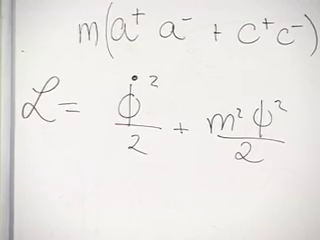
\includegraphics[width=0.62\textwidth]{lecture_07_figure_02.png}
\lectureframe{00:03:25.431}
\caption{El hamiltoniano de un modo aparece sobre el lagrangiano bosónico. La imagen conserva el signo más inicial antes de la corrección verbal a \(T-V\).}
\end{figure}

\begin{classroomqa}
\audiencequestion{¿Qué tiene de incorrecto el signo del lagrangiano del oscilador que aparece en la ecuación? \lecturetimestamp{00:04:00}}
\lecturerresponse{La energía es \(T+V\), pero el lagrangiano es \(T-V\). Por tanto, el término de potencial debe llevar un signo menos. La corrección cambia la ecuación, que pasa de describir un comportamiento exponencial a la oscilación armónica esperada.}
\end{classroomqa}

En efecto, la ecuación de Euler--Lagrange da
\begin{align}
\frac{d}{dt}\frac{\partial L_B}{\partial\dot\phi}
&=\frac{\partial L_B}{\partial\phi},\\
\ddot\phi&=-m^2\phi,
\end{align}
o bien
\begin{equation}
\ddot\phi+m^2\phi=0.
\label{eq:l7-boson-eom}
\end{equation}
Su frecuencia es \(m\), no \(m^2\). La cuantización de este oscilador produce la misma sucesión de estados descrita por \(a^\dagger\) y \(a\) en la ecuación ~\eqref{eq:l7-one-mode-hamiltonian}.

\section{Por qué la acción fermiónica es de primer orden}

El lagrangiano fermiónico parece más sencillo porque contiene una sola derivada temporal. La razón ya se aprecia en un intento deliberadamente ingenuo. Para una variable conmutativa ordinaria,
\begin{equation}
L_{\mathrm{trial}}=\phi\dot\phi
=\frac{1}{2}\frac{d}{dt}\phi^2.
\end{equation}
Es una derivada total. Su ecuación de Euler--Lagrange solo dice que \(\dot\phi=\dot\phi\), así que cualquier trayectoria diferenciable está permitida. Eliminar una derivada total de la acción cambia los datos de los extremos, pero no la ecuación de movimiento en el interior.

Ahora llamemos \(\psi\) a la variable y declarémosla impar de Grassmann. Tanto \(\psi\) como \(\dot\psi\) anticonmutan. Si se elige fijar la variación por la izquierda, reordenar los factores impares introduce un signo menos, de modo que el mismo intento formal da
\begin{equation}
\frac{d}{dt}\frac{\partial L_{\mathrm{trial}}}{\partial\dot\psi}
=\dot\psi,
\qquad
\frac{\partial L_{\mathrm{trial}}}{\partial\psi}
=-\dot\psi.
\end{equation}
Por tanto, la ecuación es
\begin{equation}
\dot\psi=-\dot\psi
\quad\Longrightarrow\quad
\dot\psi=0.
\label{eq:l7-constant-fermion}
\end{equation}
La expresión que era una tautología para una coordenada conmutativa adquiere contenido dinámico para una variable anticonmutativa. Contiene demasiado para un oscilador, pues solo permite una constante, pero precisamente ahí está la pista que necesitamos.

\begin{classroomqa}
\audiencequestion{¿La solución es simplemente que \(\psi\) es constante? \lecturetimestamp{00:13:57}}
\lecturerresponse{Sí. La ecuación~\eqref{eq:l7-constant-fermion} es una ecuación diferencial genuina de primer orden, cuya solución es una constante arbitraria con valores de Grassmann. Un término de masa convertirá esa solución estática en una oscilante.}
\end{classroomqa}

El intento obvio, \(m\psi^2\), falla porque \(\psi^2=0\). Necesitamos dos variables reales impares \(\psi_1,\psi_2\), o, de manera equivalente, una variable compleja y su conjugada. En la lección se desarrolla en la pizarra la formulación con dos variables reales, revisando una y otra vez los signos y los factores de dos. Una formulación compleja con normalización convencional es
\begin{equation}
L_F=\frac{i}{2}
\left(\bar\psi\dot\psi-\dot{\bar\psi}\psi\right)
-m\bar\psi\psi.
\label{eq:l7-fermion-lagrangian}
\end{equation}
Salvo una derivada total, esto es \(i\bar\psi\dot\psi-m\bar\psi\psi\). Al variar \(\bar\psi\) se obtiene
\begin{equation}
i\dot\psi=m\psi,
\qquad
\psi(t)=\psi(0)e^{-imt}.
\label{eq:l7-fermion-eom}
\end{equation}
La ecuación conjugada tiene la fase opuesta. Así, el modo fermiónico oscila con energía \(m\), igual que el bosónico, aunque su ecuación sea de primer orden en vez de segundo.

\editorialnote{~\eqref{eq:l7-fermion-lagrangian} fija una ordenación y normalización estándar para el cálculo exploratorio con dos variables reales. En la lección se introduce el factor \(i\), se ajusta un factor de dos y queda sin resolver el signo de una componente real. Estos cambios no alteran la conclusión central: la cinética fermiónica es de primer orden, la masa aparece linealmente y un fermión complejo proporciona un bilineal no nulo.}

Esta es la versión en dimensión cero de un contraste relativista conocido. La ecuación de Klein--Gordon es de segundo orden en el tiempo, mientras que la ecuación de Dirac es de primer orden. Al suprimir el espacio, el bosón se convierte en un oscilador armónico y el fermión en un oscilador complejo de Grassmann.

\begin{classroomqa}
\audiencequestion{¿Importa el orden en que se escriben \(\psi\), \(\dot\psi\) y sus conjugadas? \lecturetimestamp{00:18:58}}
\lecturerresponse{Las fórmulas intermedias sí dependen del orden, porque los factores impares anticonmutan. La teoría física no depende de una preferencia arbitraria al escribir, siempre que se emplee de manera coherente una misma convención para la variación por la izquierda o por la derecha, la conjugación y la integración. Invertir un par de factores impares cambia un signo, y ese signo debe cambiarse también en todo lo demás de manera coherente.}
\end{classroomqa}

Al combinar las ecuaciones ~\eqref{eq:l7-boson-lagrangian} y \eqref{eq:l7-fermion-lagrangian} obtenemos una descripción lagrangiana del mismo par degenerado representado por la ecuación ~\eqref{eq:l7-one-mode-hamiltonian}. Ya podemos identificar la simetría que los relaciona.

\section{Las cargas supersimétricas y su álgebra}

Un operador que elimina un fermión e introduce un bosón es
\begin{equation}
Q^\dagger=\sqrt{2m}\,a^\dagger c,
\end{equation}
mientras que su conjugado elimina un bosón e introduce un fermión,
\begin{equation}
Q=\sqrt{2m}\,a c^\dagger.
\end{equation}
La normalización se elige para que el álgebra adopte su forma estándar. Usando \(cc^\dagger=1-c^\dagger c\), \(aa^\dagger=a^\dagger a+1\) y el hecho de que los operadores bosónicos conmutan con los fermiónicos,
\begin{align}
\{Q,Q^\dagger\}
&=2m\left(ac^\dagger a^\dagger c+a^\dagger c a c^\dagger\right)\notag\\
&=2m\left[(a^\dagger a+1)c^\dagger c
+a^\dagger a(1-c^\dagger c)\right]\notag\\
&=2m\left(a^\dagger a+c^\dagger c\right)=2H.
\label{eq:l7-superalgebra}
\end{align}
Los operadores bosónicos pueden desplazarse a través de los fermiónicos. La misma nilpotencia que limita la ocupación fermiónica implica
\begin{equation}
Q^2=(Q^\dagger)^2=0.
\end{equation}
Por último,
\begin{equation}
[H,Q]=[H,Q^\dagger]=0.
\label{eq:l7-conserved-supercharges}
\end{equation}
Cada carga supersimétrica cambia el número de bosones y el de fermiones en sentidos opuestos, así que los dos cambios de energía se cancelan cuando las frecuencias son iguales.

\begin{classroomqa}
\audiencequestion{¿Qué es \([H,Q]\)? ¿La respuesta es proporcional a \(Q\)? \lecturetimestamp{00:25:10}}
\lecturerresponse{No. La respuesta es cero. Un operador de creación o aniquilación aislado adquiriría la energía correspondiente al conmutar con \(H\), pero las contribuciones bosónica y fermiónica en \(Q\) se cancelan. Esa cancelación se debe precisamente a la condición de igualdad de energías.}
\end{classroomqa}

\begin{classroomqa}
\audiencequestion{¿No se había escrito ya ese conmutador en la pizarra? \lecturetimestamp{00:25:45}}
\lecturerresponse{Sí. Volver a encontrarlo es útil porque nos obliga a interpretar la relación en vez de limitarnos a copiarla: conmutar con el hamiltoniano significa que la transformación es una simetría y que su generador se conserva.}
\end{classroomqa}

El adjetivo \emph{carga} alude a esta ley de conservación. Sin embargo, no debemos tratar \(Q\) como un número ordinario que pueda medirse simultáneamente y que esté asociado a un estado. Es impar de Grassmann, nilpotente y transforma un estado bosónico en uno fermiónico. Lo útil es afirmar que es un generador conservado que actúa dentro de supermultipletes degenerados.
\editorialnote{Esta formulación precisa la analogía de clase que consiste en etiquetar los estados por su energía o su carga eléctrica. Las cargas supersimétricas impares individuales no hermíticas no son observables ordinarios que tengan números cuánticos numéricos. La acción conservada de estas cargas y la representación del superálgebra completo proporcionan la clasificación adecuada.}

\section{Los generadores como derivadas}

El álgebra es compacta, pero por sí sola no nos dice cómo construir teorías con interacciones. El siguiente paso es geométrico. Los generadores de simetrías conocidos ya actúan como operadores diferenciales. Según la convención de la lección,
\begin{equation}
H=i\frac{\partial}{\partial t},
\qquad
P=-i\frac{\partial}{\partial x}.
\end{equation}

\begin{figure}[H]
\centering
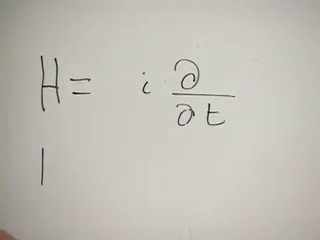
\includegraphics[width=0.50\textwidth]{lecture_07_figure_03.png}
\lectureframe{00:28:12.720}
\caption{El hamiltoniano representado como generador de las traslaciones temporales.}
\end{figure}

El momento angular también es una coordenada multiplicada por una derivada. Si las cargas supersimétricas son generadores impares, cabe preguntarse si pueden representarse mediante derivadas respecto de coordenadas impares. Por ello, ampliamos el eje temporal al supersespacio
\begin{equation}
(t,\theta,\bar\theta),
\qquad
\theta^2=\bar\theta^2=0,
\qquad
\theta\bar\theta=-\bar\theta\theta.
\end{equation}
Los campos en este espacio dependen de un tiempo ordinario y de un par conjugado de coordenadas de Grassmann.

La lección muestra deliberadamente cuán traicioneros pueden ser los signos. El signo debido a la conjugación compleja, el que aparece al mover un parámetro impar y el que resulta de elegir derivadas por la izquierda en vez de por la derecha corresponden a operaciones distintas. En lugar de conservar etapas incompatibles de la pizarra, fijaremos ahora una convención: todas las derivadas impares son por la izquierda, y
\begin{equation}
q=\partial_\theta+i\bar\theta\partial_t,
\qquad
\bar q=\partial_{\bar\theta}+i\theta\partial_t.
\label{eq:l7-differential-supercharges}
\end{equation}
Entonces
\begin{equation}
q^2=\bar q^{,2}=0,
\qquad
\{q,\bar q\}=2i\partial_t=2H.
\label{eq:l7-differential-algebra}
\end{equation}
El factor de dos procede de dos términos cruzados: \(\{\partial_\theta,\theta\}=1\) y \(\{\partial_{\bar\theta},\bar\theta\}=1\). Si los generadores solo contuvieran \(\partial_\theta\) y \(\partial_{\bar\theta}\), su anticonmutador se anularía y no podría reproducir el hamiltoniano.

\begin{classroomqa}
\audiencequestion{¿Deben llevar el mismo signo los dos términos con derivadas temporales en \(q\) y \(\bar q\)? \lecturetimestamp{00:31:01}}
\lecturerresponse{Hay que elegirlos de forma coherente para que el anticonmutador mixto sea \(2H\). Se puede usar una convención global con signo más o su alternativa conjugada coherente. El cálculo, y no la intuición visual sobre el símbolo \(i\), determina los signos relativos.}
\end{classroomqa}

En la sala se revisan los signos una y otra vez, y la dificultad acaba convirtiéndose en una broma: parece que los signos cambian durante el trayecto al trabajo. La broma viene al caso. Al hacer pasar un parámetro de Grassmann a través de una coordenada puede cambiar un signo, aunque no haya cambiado ninguna convención física. La ecuación~\eqref{eq:l7-differential-supercharges} es la referencia fija para todo lo que sigue.

\subsection{La supersimetría como desplazamiento de coordenadas}

Sean \(\xi,\bar\xi\) parámetros infinitesimales impares. La acción sobre un supercampo mediante
\begin{equation}
\delta_\xi=\xi q+\bar\xi\bar q
\end{equation}
equivale, según la convención anterior, al cambio infinitesimal de coordenadas
\begin{align}
\theta&\longrightarrow\theta+\xi,\\
\bar\theta&\longrightarrow\bar\theta+\bar\xi,\\
t&\longrightarrow t+i\left(\xi\bar\theta+\bar\xi\theta\right).
\label{eq:l7-coordinate-shift}
\end{align}
Por tanto, la variación de un supercampo escalar es
\begin{equation}
\delta_\xi\Phi
=\left(\xi\partial_\theta+\bar\xi\partial_{\bar\theta}
+i\xi\bar\theta\partial_t+i\bar\xi\theta\partial_t\right)\Phi
=\left(\xi q+\bar\xi\bar q\right)\Phi.
\end{equation}
Este es el contenido geométrico de la supersimetría. Es una traslación en direcciones impares ligada a una traslación en el tiempo ordinario. Dos desplazamientos impares se cierran en una traslación temporal, de acuerdo con la ecuación~\eqref{eq:l7-differential-algebra}.

\begin{classroomqa}
\audiencequestion{¿Podría el signo menos en disputa representar un movimiento hacia atrás en el tiempo? \lecturetimestamp{00:58:13}}
\lecturerresponse{Una convención distinta para los signos puede invertir el desplazamiento temporal infinitesimal que se muestra, pero no introduce ningún proceso físico separado de retroceso temporal. Lo que importa es que la transformación de coordenadas y los generadores diferenciales obedezcan la misma álgebra.}
\end{classroomqa}

\begin{classroomqa}
\audiencequestion{¿Tiene este tiempo extendido una realización física o es solo un artificio formal? \lecturetimestamp{00:58:23}}
\lecturerresponse{En cierto sentido útil, es un artificio formal: organiza el álgebra en una estructura geométrica. Pero esta estructura resulta físicamente valiosa al introducir interacciones. El supersespacio proporciona un cálculo sistemático para construir lagrangianos que preservan la simetría entre bosones y fermiones--en cada paso, del mismo modo que el cálculo tensorial ayuda a construir escalares de Lorentz.}
\end{classroomqa}

\section{Supercampos y la componente auxiliar}

Como solo hay dos coordenadas impares, el desarrollo de un supercampo par termina:
\begin{equation}
\Phi(t,\theta,\bar\theta)
=\phi(t)+\bar\theta\psi(t)+\bar\psi(t)\theta
+D(t)\bar\theta\theta.
\label{eq:l7-superfield}
\end{equation}
Los coeficientes de los monomios pares, \(\phi\) y \(D\), son bosónicos; los coeficientes de los monomios impares, \(\psi\) y \(\bar\psi\), son fermiónicos. No sobrevive ningún término \(\theta^2\), \(\bar\theta^2\) ni de orden superior. Dejamos sin desarrollar la dependencia temporal, porque una serie de Taylor ordinaria en \(t\) no terminaría y aquí no serviría de nada.

\begin{classroomqa}
\audiencequestion{¿Qué representa la componente \(D(t)\) del término de orden superior? \lecturetimestamp{00:41:46}}
\lecturerresponse{En esta etapa es simplemente el coeficiente bosónico final del desarrollo finito. En la acción por componentes normalmente no tiene término cinético y se elimina mediante una ecuación de movimiento algebraica; por eso se llama campo auxiliar. En tono jocoso, la lección sugiere ``D de «dummy»,'' que expresa su papel no dinámico, aunque esa no sea la definición histórica.}
\end{classroomqa}

El supercampo es un solo objeto, mientras que \(\phi,\psi,\bar\psi,D\) son sus componentes. Una transformación supersimétrica los mezcla. Así, un bosón y un fermión están relacionados de una manera estructural muy parecida a la relación entre las componentes \(x\) y \(y\) de un vector bajo una rotación, aunque las direcciones de Grassmann no puedan representarse como ejes ordinarios.

\section{La superacción y la componente de orden superior}

Para obtener ecuaciones de movimiento necesitamos una acción. En teoría de campos ordinaria se forma un lagrangiano escalar y se integra sobre el espacio-tiempo. Aquí, la expresión análoga es
\begin{equation}
S=\int dt\,d\theta\,d\bar\theta\;\Lambda
\bigl(\Phi,\text{ superspace derivatives of }\Phi\bigr),
\label{eq:l7-superaction}
\end{equation}
donde \(\Lambda\) es un supercampo par. La integración de Berezin es algebraica. Elegimos
\begin{equation}
\int d\theta\,d\bar\theta\;\bar\theta\theta=1.
\end{equation}
Por tanto, si
\begin{equation}
\Lambda=A+\bar\theta B+\bar B\theta+C\bar\theta\theta,
\end{equation}
entonces
\begin{equation}
\int d\theta\,d\bar\theta\;\Lambda=C.
\label{eq:l7-top-component}
\end{equation}
La integración respecto de las coordenadas impares extrae la componente de orden superior y deja un lagrangiano ordinario que se integra respecto del tiempo.

¿Por qué es invariante el resultado? Una variación supersimétrica traslada las variables de integración. La variación de la componente de orden superior es una derivada total ordinaria respecto del tiempo, mientras que las derivadas totales impares se anulan al integrar según Berezin. Con condiciones adecuadas en los extremos, la acción no cambia. Este es el análogo en el supersespacio de construir un escalar de Lorentz antes de integrarlo sobre el espacio-tiempo.

\section{Producto de supercampos}

La manera más sencilla de obtener un supercampo nuevo a partir de uno dado es multiplicarlo por sí mismo. Partiendo de la ecuación~\eqref{eq:l7-superfield}, se anula todo término que contenga \(\theta^2\) o \(\bar\theta^2\). Manteniendo el orden \(\bar\theta\theta\) y colocando a la izquierda los campos componentes con barra, obtenemos
\begin{align}
\Phi^2
={}&\phi^2
+2\phi\bar\theta\psi
+2\phi\bar\psi\theta\notag\\
&+\left(2\phi D-2\bar\psi\psi\right)\bar\theta\theta.
\label{eq:l7-superfield-square}
\end{align}

\begin{figure}[H]
\centering
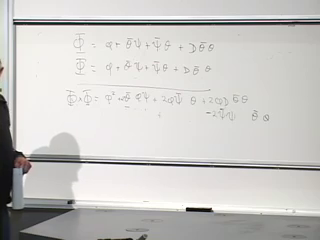
\includegraphics[width=0.82\textwidth]{lecture_07_figure_05.png}
\lectureframe{01:07:57.844}
\caption{El producto de supercampos componente a componente y la colección de sus términos \(\bar\theta\theta\).}
\end{figure}

Los dos términos \(\phi D\) y \(D\phi\) se suman porque ambos campos son pares. Los dos términos cruzados fermiónicos también se suman después de reordenar cada uno, pero ambos llevan el mismo signo negativo:
\begin{equation}
(\bar\theta\psi)(\bar\psi\theta)
+(\bar\psi\theta)(\bar\theta\psi)
=-2\bar\psi\psi\,\bar\theta\theta.
\end{equation}
Al integrar el cuadrado respecto de las coordenadas impares se obtiene
\begin{equation}
\int d\theta\,d\bar\theta\;\Phi^2
=2\phi D-2\bar\psi\psi.
\end{equation}
Este término es supersimétrico por construcción, pero aún no es un lagrangiano cinético. No contiene derivadas temporales.

A continuación, en la pizarra se proponen \(\Phi^3\), \(\Phi^4\) y \(\Phi^n\) como ejercicios. Hay una regla compacta. Para cualquier función ordinaria \(W\),
\begin{equation}
\left.W(\Phi)\right|_{\bar\theta\theta}
=W'(\phi)D-W''(\phi)\bar\psi\psi.
\label{eq:l7-function-top-component}
\end{equation}
Para \(W(\phi)=\phi^2\), esto reproduce la ecuación~\eqref{eq:l7-superfield-square}; para \(W(\phi)=\phi^n\), da
\begin{equation}
\left.\Phi^n\right|_{\bar\theta\theta}
=n\phi^{n-1}D-n(n-1)\phi^{n-2}\bar\psi\psi.
\end{equation}
\editorialnote{La lección propone como ejercicio la potencia \(n\) y anticipa qué tipos de términos cabe esperar. La ecuación~\eqref{eq:l7-function-top-component} proporciona la regla completa con la convención de orden fijada.}

En este punto, el profesor pregunta si el público está agotado. El público responde que no; él contesta que sí lo está. El intercambio es algo más que un alivio cómico. Las potencias de supercampos son fáciles porque el desarrollo termina, pero las derivadas y las restricciones son donde la contabilidad de signos se vuelve realmente exigente.

\section{¿Qué derivadas respetan la supersimetría?}

Antes de seguir el siguiente argumento de la pizarra, hay que hacer una corrección. La derivada temporal ordinaria no plantea ningún problema:
\begin{equation}
[\partial_t,q]=[\partial_t,\bar q]=0.
\end{equation}
Por consiguiente, \(\partial_t\Phi\) se transforma como un supercampo siempre que lo haga \(\Phi\). Los objetos sutiles son las derivadas impares sin modificar \(\partial_\theta\Phi\) y \(\partial_{\bar\theta}\Phi\), porque no anticonmutan con ambas cargas supersimétricas. Necesitamos derivadas impares modificadas para las restricciones y para construir componentes de manera manifiestamente supersimétrica.
\editorialnote{La afirmación verbal de que la derivación temporal no produce otro supercampo no es correcta con la convención que usamos aquí. Como \(\partial_t\) conmuta con ambas cargas supersimétricas, es covariante. La construcción posterior de derivadas impares modificadas sigue siendo necesaria y constituye el verdadero punto matemático de la lección.}

\subsection{La analogía del campo «mágico»``''}

La lección motiva el criterio mediante rotaciones ordinarias. Sea \(f(x,y)\) tal que
\begin{equation}
\partial_y f=0.
\label{eq:l7-magic-constraint}
\end{equation}
Llamemos a una función así campo ``«mágico».'' Depende de \(x\), pero no de \(y\). ¿Se conserva la clase de campos mágicos bajo rotaciones? Para
\begin{equation}
L_z=-i\left(x\partial_y-y\partial_x\right),
\end{equation}
obtenemos
\begin{equation}
[\partial_y,L_z]=i\partial_x\neq0.
\end{equation}
Por tanto, \(L_z f\) en general adquiere dependencia respecto de \(y\), aunque \(f\) satisfaga inicialmente la ecuación~\eqref{eq:l7-magic-constraint}. La restricción no es invariante bajo rotaciones.

La lección general es sencilla. Si un campo satisface \(C\Phi=0\) y una simetría está generada por \(G\), el campo transformado sigue satisfaciendo la restricción cuando el conmutador graduado de \(C\) y \(G\) se anula. Para dos operadores impares, el conmutador graduado es un anticonmutador.

\begin{classroomqa}
\audiencequestion{¿Cuándo es compatible con una simetría una restricción impuesta a un campo? \lecturetimestamp{01:17:56}}
\lecturerresponse{Cuando el operador de restricción conmuta en sentido graduado con los generadores de simetría. Entonces se puede desplazar \(C(G\Phi)\) a través de \(G\) y reducirlo a \(G(C\Phi)=0\). El ejemplo de la rotación falla porque \(\partial_y\) no conmuta con el generador de rotaciones.}
\end{classroomqa}

\subsection{Derivadas impares covariantes}

Con las cargas supersimétricas fijadas por la ecuación~\eqref{eq:l7-differential-supercharges}, definimos
\begin{equation}
\mathcal D=\partial_\theta-i\bar\theta\partial_t,
\qquad
\bar{\mathcal D}=\partial_{\bar\theta}-i\theta\partial_t.
\label{eq:l7-covariant-derivatives}
\end{equation}
El único cambio es el signo del término con derivada temporal. El cálculo directo da
\begin{align}
\{\mathcal D,q\}
&=\{\mathcal D,\bar q\}
=\{\bar{\mathcal D},q\}
=\{\bar{\mathcal D},\bar q\}=0,\\
\{\mathcal D,\bar{\mathcal D}\}&=-2i\partial_t.
\label{eq:l7-covariant-algebra}
\end{align}
Los dos términos cruzados potencialmente no nulos se cancelan. Es el análogo impar de una derivada covariante: deriva preservando la ley de transformación.

En la lección se usa \(D\) tanto para la componente auxiliar como para esta derivada. Reservamos \(D(t)\) para la componente y usamos la letra caligráfica \(\mathcal D\) para el operador.

\section{La restricción quiral}

Ahora podemos imponer una restricción no trivial que se conserva bajo la supersimetría:
\begin{equation}
\bar{\mathcal D}\Phi=0.
\label{eq:l7-chiral-constraint}
\end{equation}
Un campo que la satisface se llama quiral. Si es quiral antes de una transformación supersimétrica, entonces
\begin{equation}
\bar{\mathcal D}(q\Phi)
=-q(\bar{\mathcal D}\Phi)=0,
\qquad
\bar{\mathcal D}(\bar q\Phi)
=-\bar q(\bar{\mathcal D}\Phi)=0.
\end{equation}
Así, el supercampo transformado entero permanece dentro de la clase restringida. A diferencia de la condición de campo mágico, la quiralidad es compatible con la simetría.

Para resolver la restricción, definimos una coordenada temporal desplazada
\begin{equation}
\tau=t+i\bar\theta\theta.
\label{eq:l7-chiral-time}
\end{equation}
Como usamos derivadas por la izquierda,
\begin{equation}
\partial_{\bar\theta}\tau=i\theta,
\end{equation}
y, por tanto,
\begin{equation}
\bar{\mathcal D}F(\tau,\theta)
=\left(\partial_{\bar\theta}-i\theta\partial_t\right)F(\tau,\theta)
=i\theta\partial_\tau F-i\theta\partial_\tau F=0.
\end{equation}
Así pues, el supercampo quiral local más general depende de \(\bar\theta\) solo a través de \(\tau\):
\begin{equation}
\Phi_{\mathrm{ch}}(\tau,\theta)
=\phi(\tau)+\bar\psi(\tau)\theta.
\label{eq:l7-chiral-field-tau}
\end{equation}

\begin{classroomqa}
\audiencequestion{¿Depender de \(\tau\) y \(\theta\) es la única forma de satisfacer la restricción quiral? \lecturetimestamp{01:32:35}}
\lecturerresponse{Localmente, sí. La ecuación diferencial \(\bar{\mathcal D}\Phi=0\) dice precisamente que la dependencia independiente respecto de \(\bar\theta\) puede incorporarse a la coordenada desplazada \(\tau=t+i\bar\theta\theta\). El desarrollo finito restante es una función de \(\tau\) más un término proporcional a \(\theta\).}
\end{classroomqa}

Al volver a desarrollar en la coordenada temporal original,
\begin{align}
\phi(\tau)
&=\phi(t)+i\bar\theta\theta\dot\phi(t),\\
\bar\psi(\tau)\theta
&=\bar\psi(t)\theta,
\end{align}
pues la corrección a la segunda línea contiene \(\theta^2\). Así,
\begin{equation}
\Phi_{\mathrm{ch}}(t,\theta,\bar\theta)
=\phi(t)+\bar\psi(t)\theta
+i\bar\theta\theta\dot\phi(t).
\label{eq:l7-chiral-field-components}
\end{equation}

\begin{classroomqa}
\audiencequestion{¿Debe incluir un término de segundo orden el desarrollo de Taylor de \(\phi(t+i\bar\theta\theta)\)? \lecturetimestamp{01:33:51}}
\lecturerresponse{No. La primera corrección es \(i\bar\theta\theta\dot\phi\), y todas las correcciones de orden superior contienen \((\bar\theta\theta)^2=0\). El público lo advierte enseguida: la nilpotencia ya había dado los dos primeros términos y había truncado la serie.}
\end{classroomqa}

Esta es la economía de la quiralidad. El supercampo sin restricciones de la ecuación~\eqref{eq:l7-superfield} tiene dos componentes bosónicas y dos fermiónicas. En este ejemplo mínimo unidimensional, la condición quiral elimina la componente auxiliar independiente y relaciona la componente de orden superior con \(\dot\phi\).

\section{El cálculo que, con razón, se interrumpe}

El siguiente paso natural es combinar el campo quiral con su conjugado e integrar en el supersespacio. Se empieza a escribir el desarrollo conjugado, y alguien del público pregunta si el orden \(\theta\bar\theta\) debe invertirse al conjugar. En ese momento, los signos dejan de parecer fiables. En vez de fingir seguridad, se interrumpe el cálculo.

\begin{classroomqa}
\audiencequestion{¿Podemos conocer el resultado principal aunque se posponga la multiplicación por el campo conjugado? \lecturetimestamp{01:37:30}}
\lecturerresponse{Sí. Si se tratan de manera coherente los signos y las conjugaciones, una expresión en el supersespacio construida a partir de un campo quiral y su conjugado produce los términos cinéticos bosónico y fermiónico ordinarios deseados. El resultado importante de esta lección es el principio de construcción, no una línea final poco fiable copiada de un cálculo hecho con cansancio.}
\end{classroomqa}

Conviene dejar visible el punto en que se interrumpe el cálculo. El formalismo no perdona: basta colocar mal un factor impar para cambiar un signo, y hay que conservar la misma convención al conjugar, derivar, multiplicar e integrar. Si se pierde esa coherencia, lo correcto es restablecerla antes de continuar. En una convención estándar, la acción cinética conocida se construye a partir de un producto con el campo conjugado, pero su reducción detallada por componentes corresponde al siguiente cálculo, hecho con cuidado, no a una reconstrucción de una línea inacabada de la pizarra.

\section{Por qué la simetría es la idea central}

Un lagrangiano supersimétrico hace más que colocar un bosón junto a un fermión. Restringe sus masas e interacciones para que formen una representación del superálgebra. En un vacío exactamente supersimétrico, los miembros de un supermultiplete tienen masas iguales. Sus contribuciones de lazos están correlacionadas, y los efectos ultravioleta bosónicos y fermiónicos se cancelan precisamente en las combinaciones impuestas por la simetría.

Por eso importa el aparato de construcción. Se podrían enumerar los vértices de Feynman y verificar las cancelaciones diagrama por diagrama, pero entonces estas parecerían accidentales. La supersimetría las explica del mismo modo que la simetría de Lorentz explica por qué las amplitudes de dispersión se transforman coherentemente en todos los sistemas de referencia inerciales.

\editorialnote{La supersimetría exacta no implica que se anule cada corrección individual a la autoenergía. Relaciona las renormalizaciones y elimina ciertas sensibilidades ultravioletas; los enunciados de no renormalización dependen de la magnitud, la dimensión y la cantidad de supersimetría. Se conserva aquí la afirmación amplia de la lección sobre las cancelaciones, expresada con estas salvedades.}

\begin{classroomqa}
\audiencequestion{¿Cómo se escribe ``«quiral»''? \lecturetimestamp{01:39:48}}
\lecturerresponse{Q-U-I-R-A-L. La palabra designa la restricción \(\bar{\mathcal D}\Phi=0\); no se refiere a la quiralidad geométrica ordinaria de un objeto en el espacio tridimensional, aunque la terminología provenga de la estructura levógira y dextrógira de los espinores relativistas.}
\end{classroomqa}

\begin{classroomqa}
\audiencequestion{¿Se podría prescindir del lagrangiano e ir directamente a las reglas de Feynman supersimétricas? \lecturetimestamp{01:40:00}}
\lecturerresponse{Desde luego, se pueden enunciar las reglas, pero entonces las relaciones entre los acoplamientos y las cancelaciones que producen parecen coincidencias sin explicación. El contenido más profundo es la simetría del espacio-tiempo generalizada. El lagrangiano, o una formulación invariante equivalente, hace visible esa razón y genera las reglas de forma sistemática.}
\end{classroomqa}

Supongamos que todos los órdenes perturbativos dieran amplitudes invariantes de Lorentz, aunque no se hubiera mencionado ninguna transformación de Lorentz. Tras suficientes cálculos, exigiríamos una explicación. La respuesta sería la simetría del espacio-tiempo que organiza de una vez todos los órdenes. El papel del superspacio es análogo: los desplazamientos en \(\theta,\bar\theta\) mezclan componentes bosónicas y fermiónicas, y su álgebra se cierra sobre las traslaciones en el espacio-tiempo.

\begin{classroomqa}
\audiencequestion{¿También habría que desarrollar las coordenadas espaciales ordinarias en una serie de potencias finita, como se hace con las coordenadas de Grassmann? \lecturetimestamp{01:44:55}}
\lecturerresponse{No. Una serie de potencias de una coordenada ordinaria no termina y, por lo general, no es la descomposición natural. Una transformada de Fourier resulta más útil porque descompone un campo en ondas y momentos. El desarrollo en \(\theta\) es especial precisamente porque la nilpotencia lo hace finito.}
\end{classroomqa}

\begin{classroomqa}
\audiencequestion{Si apareciera una partícula nueva en el LHC, ¿cómo podríamos saber si es una supercompañera y no simplemente una partícula desconocida? \lecturetimestamp{01:45:42}}
\lecturerresponse{La supersimetría predice números cuánticos e interacciones correlacionados, no solo un estado adicional. Los espines difieren en una unidad de un medio, las cargas gauge están relacionadas y muchos acoplamientos cúbicos y cuárticos dependen de menos parámetros independientes que en una teoría genérica. Las secciones eficaces, las fracciones de ramificación y el resto del espectro tendrían que satisfacer esas relaciones.}
\end{classroomqa}

Una resonancia desconocida por sí sola no demostraría la supersimetría. Sí lo haría una red de relaciones entre acoplamientos y elementos del espectro. Esa es la contraparte experimental de la construcción del superspacio: interacciones entre componentes que parecen independientes proceden de un único objeto invariante.

\begin{classroomqa}
\audiencequestion{Las partículas observadas y sus hipotéticas supercompañeras no tienen la misma masa. ¿Cómo cambia eso la teoría? \lecturetimestamp{01:47:01}}
\lecturerresponse{La cambia enormemente. La supersimetría debe romperse, por lo general mediante una ruptura espontánea que se transmite al sector observado. La ruptura separa las masas de los miembros de un supermultiplete, pero conserva suficiente estructura para controlar las interacciones y, si la escala es lo bastante baja, las correcciones ultravioletas. Desarrollar ese mecanismo constituye una teoría sustancial por sí misma, sobre todo cuando se incluye la gravedad.}
\end{classroomqa}

\section{Un principio sencillo, un cálculo difícil}

La valoración final es inusualmente franca. La idea inicial parece sencilla: los bosones y los fermiones están relacionados por una simetría. Sin embargo, llevarla a la práctica pronto exige dominar índices, conjugaciones, ordenamientos de Grassmann y signos. Incluso después de construir la simetría, la física de partículas realista requiere romperla; acoplarla a la gravedad conduce hacia la supergravedad y añade otra capa de estructura.

Esta dificultad no demuestra que la idea esté vacía. La naturaleza no tiene por qué hacer que un principio sencillo sea fácil de calcular. Los especialistas aprenden el tema repitiendo los detalles hasta que las reglas de los signos se vuelven automáticas. La frustración nace de la distancia entre el álgebra compacta
\begin{equation}
\{Q,Q^\dagger\}=2H
\end{equation}
y toda la maquinaria necesaria para realizarla en una teoría con interacciones.

\begin{classroomqa}
\audiencequestion{¿Una capa adicional de abstracción acaba simplificando el formalismo, o las complicaciones siguen acumulándose? \lecturetimestamp{01:49:33}}
\lecturerresponse{Ninguna simplificación general ha eliminado el trabajo detallado. Las reglas subyacentes pueden ser breves, pero aplicarlas de manera fiable exige dominar repetidamente las convenciones. Por eso, un tratamiento completo suele ocupar un curso técnico entero, en lugar de una fracción de un curso general de física de partículas.}
\end{classroomqa}

\begin{classroomqa}
\audiencequestion{¿Las transformaciones nos dicen qué son realmente los fermiones y los bosones, o por qué su comportamiento ordinario es diferente? \lecturetimestamp{01:51:42}}
\lecturerresponse{Nos dicen que ambos son componentes de un único supercampo e imágenes uno del otro bajo la acción de las supercargas. La acción de \(Q\) transforma un componente bosónico en uno fermiónico, mientras que la transformación siguiente produce derivadas y componentes auxiliares. Esto es análogo a una rotación que mezcla componentes de un vector, pero no puede traducirse en una imagen igual de literal: el lenguaje adecuado es la propia geometría de Grassmann.}
\end{classroomqa}

Esa respuesta nos devuelve a la idea central. Una transformación de supersimetría es un pequeño desplazamiento en el superspacio. Mezcla \(\phi,\psi,\bar\psi,D\) igual que una rotación ordinaria mezcla componentes, y lo hace de modo que el álgebra se cierra sobre una traslación temporal. La imagen es abstracta, pero no arbitraria: cada término del supercampo, cada signo de las derivadas covariantes y cada relación entre las interacciones de los componentes están ahí para realizar el álgebra.

\section{Lo que hemos construido}

Partimos del hamiltoniano del oscilador emparejado y recuperamos sus dos descripciones lagrangianas diferentes. El bosón obedece una ecuación de oscilador de segundo orden; el fermión requiere una acción de Grassmann de primer orden y un par complejo de componentes impares. Las supercargas intercambian los dos modos, cada una se anula al elevarla al cuadrado, anticonmutan para dar el hamiltoniano y conmutan con él.

Representar esas cargas mediante operadores diferenciales nos condujo al superspacio. El desarrollo finito de un supercampo reunió componentes bosónicos, fermiónicos y auxiliares; la integración de Berezin seleccionó el componente de grado máximo de un superlagrangiano; y la multiplicación generó posibles interacciones invariantes. La exigencia de una diferenciación impar compatible con la simetría condujo entonces a \(\mathcal D,\bar{\mathcal D}\), a la restricción quiral y a la coordenada desplazada \(\tau=t+i\bar\theta\theta\).

El cálculo inconcluso del producto conjugado forma parte de la lección, no es un defecto que haya que ocultar. La supersimetría comienza con una exigencia física sencilla, pero su cálculo es sensible a cada elección de ordenamiento. Una vez que se controlan esas elecciones, la recompensa es poderosa: la simetría organiza las masas y los acoplamientos, las correcciones cuánticas satisfacen relaciones que no son accidentales, y los bosones y los fermiones se convierten en componentes de un único objeto geométrico.

\chapter{Supersimetría en cuatro dimensiones y el modelo de Wess--Zumino}

\lectureoverview{El álgebra de supersimetría unidimensional de la lección anterior incluía únicamente el Hamiltoniano. La invariancia de Lorentz obliga ahora a reincorporar la energía junto con el momento espacial, y las cargas supersimétricas deben convertirse en espinores de dos componentes. Llegamos a esa álgebra retomando primero un fermión de Weyl sin masa y su Hamiltoniano \(H=\boldsymbol{\sigma}\cdot\mathbf p\). Luego representamos las cargas supersimétricas como operadores diferenciales en el superspacio de cuatro dimensiones, aislamos los supercampos quirales mediante la condición \(\bar D_{\dot\alpha}\Phi=0\) y usamos la integración en superspacio para construir una teoría de campos concreta. Las elecciones sucesivas \(\Phi^\dagger\Phi\), \(\Phi^2\) y \(\Phi^3\) producen propagación, masas iguales para bosones--fermiones, interacciones de Yukawa y una interacción escalar relacionada. El campo auxiliar \(F\) hace transparentes estas relaciones, mientras que los diagramas de lazo finales muestran por qué la supersimetría suaviza la sensibilidad ultravioleta.}

\section{Por qué el hamiltoniano no puede estar solo}

En el modelo de juguete se suprimió el espacio y la relación básica era
\begin{equation}
\{Q,Q^\dagger\}=2H.
\label{eq:l8-time-only-algebra}
\end{equation}
Esta forma basta cuando el tiempo es la única coordenada. Sin embargo, en una teoría relativista, \(H=P_0\) es una componente del cuadrimomento \(P_\mu\). Un impulso de Lorentz la mezcla con \(P_i\). Un álgebra cuyo lado derecho destacara \(P_0\) no podría transformarse de manera covariante.

Por tanto, la corrección debe cumplir dos propósitos a la vez. Debe sustituir \(H\) por las cuatro componentes \(P_\mu\) y proporcionar índices en el lado izquierdo que puedan corresponderse con un vector de Lorentz en el lado derecho. La ecuación de Dirac sin masa da la pista necesaria: un fermión relativista puede describirse mediante un espinor de dos componentes, y las matrices \(\sigma^\mu\) convierten un índice vectorial en un par de índices espinoriales.

\section{Fermiones sin masa, helicidad y quiralidad}

Empecemos por la distinción física entre partículas masivas y sin masa. Consideremos una partícula de espín \(\tfrac12\) que se mueve en la dirección de su espín. Como su velocidad es menor que la de la luz, un observador puede adelantarla. En el nuevo sistema de referencia, el momento se invierte, pero el espín no, así que la helicidad cambia de signo. Por consiguiente, una teoría relativista de partículas masivas debe contener ambas helicidades.

Ningún observador puede adelantar una partícula sin masa. Las transformaciones propias de Lorentz no pueden invertir su momento con respecto al espín, de modo que una representación irreducible sin masa puede tener una sola helicidad. Una rotación espacial puede cambiar la dirección del movimiento, pero no convierte una mano derecha en una izquierda.

\begin{classroomqa}
\audiencequestion{¿El argumento de adelantar a la partícula se refiere realmente a la helicidad y no a la quiralidad? \lecturetimestamp{00:05:42}}
\lecturerresponse{Sí. La helicidad es la proyección del espín sobre el momento, mientras que la quiralidad es el autovalor de la matriz quiral, convencionalmente \(\gamma^5\). Para un modo sin masa, ambas etiquetas están vinculadas, por eso en este ejemplo pueden parecer intercambiables. Para una partícula masiva son distintas.}
\end{classroomqa}

El recuento de estados requiere una precisión.\editorialnote{Un único campo de Weyl sin masa tiene una helicidad para la partícula y la helicidad opuesta para la antipartícula. Por tanto, «la mitad de estados» se refiere a la reducción de un campo de Dirac de cuatro componentes a un campo de Weyl de dos componentes; no significa que hayan desaparecido los estados de antipartícula.}

Escribamos el campo de Weyl empleado en este argumento inicial como
\begin{equation}
\chi=
\begin{pmatrix}
\chi_1\\
\chi_2
\end{pmatrix},
\end{equation}
En la clase, este campo se denota por \(\psi_\alpha\); aquí lo llamamos \(\chi\) para no confundirlo con la representación de Weyl conjugada que suele incluirse más adelante en un supercampo quiral.
\begin{equation}
H\chi=\boldsymbol{\sigma}\cdot\mathbf p\,\chi.
\label{eq:l8-weyl-hamiltonian}
\end{equation}
Para el momento \(\mathbf p\), la matriz \(\boldsymbol{\sigma}\cdot\mathbf p\) tiene autovalores \(\pm|\mathbf p|\). La rama de frecuencia positiva proporciona el modo de partícula; la rama de frecuencia negativa se reinterpreta mediante la construcción de la antipartícula, en vez de conservarse como un espectro no acotado inferiormente.

\begin{figure}[H]
\centering
\includegraphics[width=0.70\textwidth]{lecture_08_figure_02.png}
\lectureframe{00:07:44.271}
\caption{El espinor quiral de dos componentes y el hamiltoniano \(H=\boldsymbol{\sigma}\cdot\mathbf p\). El símbolo del momento al final está parcialmente oculto, pero la ecuación pronunciada lo determina.}
\end{figure}

La etiqueta de quiralidad también depende de la convención.\editorialnote{La pizarra asocia directamente una quiralidad con el autovalor positivo de \(\boldsymbol{\sigma}\cdot\mathbf p\). La quiralidad que recibe ese signo depende de las definiciones de \(\sigma^\mu\), \(\bar\sigma^\mu\) y del campo de Weyl. Conservamos la afirmación sobre el autovalor, pero no le asignamos una etiqueta izquierda/derecha independiente de la convención.}

Al sustituir \(H\) por \(i\partial_t\) y \(\mathbf p\) por \(-i\nabla\), obtenemos
\begin{equation}
i\partial_t\chi=-i\boldsymbol{\sigma}\cdot\nabla\chi.
\end{equation}
Introduzcamos
\begin{equation}
\begin{aligned}
\sigma^\mu&=(\mathbf 1,\boldsymbol{\sigma}),\\
\bar\sigma^\mu&=(\mathbf 1,-\boldsymbol{\sigma}),\\
\eta_{\mu\nu}&=\operatorname{diag}(1,-1,-1,-1).
\end{aligned}
\label{eq:l8-sigma-convention}
\end{equation}
Entonces, la ecuación que acabamos de obtener es
\begin{equation}
i\sigma^\mu\partial_\mu\chi=0.
\label{eq:l8-weyl-equation}
\end{equation}
La representación de Weyl conjugada usa \(\bar\sigma^\mu\). Es esta representación conjugada, que denotaremos \(\psi_\alpha\) más adelante, la que satisface la ecuación libre \(i\bar\sigma^\mu\partial_\mu\psi=0\). Demostrar la covariancia requiere la representación espinorial del grupo de Lorentz, pero aquí importa el hecho estructural: las cuatro matrices \(\sigma^\mu\) enlazan un índice del espacio-tiempo con dos índices espinoriales.

\section{El superálgebra en cuatro dimensiones}

Las coordenadas impares deben transformarse ahora como espinores de Weyl:
\begin{equation}
\theta^\alpha=(\theta^1,\theta^2),
\qquad
\bar\theta^{\dot\alpha}=(\bar\theta^{\dot1},\bar\theta^{\dot2}).
\end{equation}
La barra denota conjugación compleja, y el punto distingue la representación de Lorentz conjugada. Hay dos componentes complejas, o cuatro reales, de Grassmann. Por tanto, un supercampo par general
\begin{equation}
\mathcal S=\mathcal S(x^\mu,\theta^\alpha,\bar\theta^{\dot\alpha})
\end{equation}
tiene un desarrollo finito en Grassmann. Su monomio de grado máximo es
\begin{equation}
\theta^2\bar\theta^2
\equiv
(\theta^1\theta^2)(\bar\theta^{\dot1}\bar\theta^{\dot2}),
\end{equation}
el producto de las cuatro coordenadas impares independientes. Al coeficiente de este monomio se le llama comúnmente componente \(D\).

Las supercargas también llevan índices espinoriales. En la supersimetría \(N=1\) de cuatro dimensiones, su álgebra es
\begin{align}
\{Q_\alpha,\bar Q_{\dot\beta}\}
&=2\sigma^\mu_{\alpha\dot\beta}P_\mu,
\label{eq:l8-superalgebra-main}\\
\{Q_\alpha,Q_\beta\}&=0,
&
\{\bar Q_{\dot\alpha},\bar Q_{\dot\beta}\}&=0,
\label{eq:l8-superalgebra-nilpotent}\\
[P_\mu,Q_\alpha]&=0,
&
[P_\mu,\bar Q_{\dot\alpha}]&=0,
&
[P_\mu,P_\nu]&=0.
\label{eq:l8-superalgebra-commutators}
\end{align}
El factor dos es convencional. La matriz
\(\sigma^\mu_{\alpha\dot\beta}\) contrae el índice vectorial de \(P_\mu\) y deja precisamente los dos índices espinoriales que aparecen a la izquierda.

\begin{classroomqa}
\audiencequestion{¿Son \(\alpha\) y \(\beta\) los índices matriciales de la matriz sigma? \lecturetimestamp{00:22:01}}
\lecturerresponse{Sí. Más precisamente, uno es un índice de Weyl sin punto y el otro, un índice conjugado con punto; \(\mu\) es el índice de vector del espacio-tiempo. La matriz sigma sirve de puente entre ambas descripciones.}
\end{classroomqa}

La notación depurada hace explícito ese puente.\editorialnote{En la clase se omiten deliberadamente los índices con punto y se debate en la pizarra el orden \(\alpha\beta\) frente a \(\beta\alpha\). Las ecuaciones~\eqref{eq:l8-superalgebra-main} y \eqref{eq:l8-superalgebra-commutators} restablecen la notación estándar con índices con y sin punto, sin cambiar el argumento.}

La última línea afirma que las supercargas se conservan y son compatibles con las traslaciones. Las componentes del momento conmutan porque sus representantes diferenciales conmutan. En la convención diferencial que usaremos más adelante,
\begin{equation}
P_\mu=i\partial_\mu,
\end{equation}
por lo que la ecuación~\eqref{eq:l8-superalgebra-main} también puede escribirse como
\begin{equation}
\{Q_\alpha,\bar Q_{\dot\beta}\}
=2i\sigma^\mu_{\alpha\dot\beta}\partial_\mu.
\end{equation}

\section{Supercargas como derivadas en el superspacio}

El momento genera traslaciones de una coordenada ordinaria; una supercarga traslada una coordenada impar y, además, desplaza el espacio-tiempo. Fijemos la convención de derivadas de Grassmann por la izquierda y definamos
\begin{align}
Q_\alpha
&=\partial_\alpha
-i\sigma^\mu_{\alpha\dot\alpha}
\bar\theta^{\dot\alpha}\partial_\mu,
\label{eq:l8-Q}\\
\bar Q_{\dot\alpha}
&=-\bar\partial_{\dot\alpha}
+i\theta^\alpha\sigma^\mu_{\alpha\dot\alpha}\partial_\mu.
\label{eq:l8-Qbar}
\end{align}
La acción de \(\epsilon^\alpha Q_\alpha+
\bar\epsilon_{\dot\alpha}\bar Q^{\dot\alpha}\) da la variación infinitesimal de supersimetría de un supercampo. Sus componentes son simplemente los coeficientes de los monomios independientes de Grassmann, y los operadores diferenciales mezclan esos coeficientes.

\begin{classroomqa}
\audiencequestion{¿A qué derivada respecto de \(x\) se refiere la abreviatura \(\bar\theta\sigma\partial\)? \lecturetimestamp{00:25:40}}
\lecturerresponse{A las cuatro. El índice \(\mu\) repetido en \(\bar\theta^{\dot\alpha}\sigma^\mu_{\alpha\dot\alpha}\partial_\mu\) está sumado, de modo que cada componente de \(\sigma^\mu\) se empareja con la derivada correspondiente \(\partial/\partial x^\mu\).}
\end{classroomqa}

\begin{classroomqa}
\audiencequestion{¿La carga conjugada debería contener \(\theta\) en vez de otro \(\bar\theta\)? \lecturetimestamp{00:26:16}}
\lecturerresponse{Sí. \(Q\) deriva con respecto a \(\theta\) y contiene \(\bar\theta\); \(\bar Q\) deriva con respecto a \(\bar\theta\) y contiene \(\theta\). Son operadores conjugados.}
\end{classroomqa}

\begin{classroomqa}
\audiencequestion{¿Es simétrica \(\sigma^\mu\)? \lecturetimestamp{00:27:04}}
\lecturerresponse{Las matrices de Pauli son hermíticas. Tres de las cuatro matrices de \((\mathbf1,\boldsymbol{\sigma})\) son simétricas, mientras que \(\sigma^2\) es antisimétrica bajo la transposición ordinaria. La propiedad de conjugación relevante es la hermiticidad junto con la posición de los índices con y sin punto.}
\end{classroomqa}

\begin{classroomqa}
\audiencequestion{¿La matriz sigma de la ecuación conjugada lleva los índices en el orden opuesto? \lecturetimestamp{00:27:13}}
\lecturerresponse{La conjugación intercambia las representaciones con y sin punto, así que la notación segura es \(\sigma^\mu_{\alpha\dot\alpha}\) y su conjugada \(\bar\sigma^{\mu\,\dot\alpha\alpha}\), en lugar de tratar ambas etiquetas como posiciones matriciales intercambiables.}
\end{classroomqa}

Las fórmulas de las ecuaciones~\eqref{eq:l8-Q} y \eqref{eq:l8-Qbar} difieren en signos superficiales respecto de la abreviatura usada en la pizarra. Esos signos dependen de si \(P_\mu\) es \(+i\partial_\mu\) o \(-i\partial_\mu\), de si las derivadas actúan por la izquierda o por la derecha y del orden de las variables impares conjugadas. Lo importante es que una misma convención satisfaga toda el álgebra.

\section{Una restricción compatible con la supersimetría}

Un supercampo general contiene muchas componentes. Buscamos una clase más reducida sin destruir la simetría. La clase comienza con una analogía ordinaria. Para un vector \(\mathbf V\), la restricción
\begin{equation}
V_x=0
\end{equation}
no es invariante bajo rotaciones: después de una rotación, \(V_y\) contribuye a la nueva componente \(x\). En cambio,
\begin{equation}
\mathbf V^2=1
\end{equation}
es invariante y elimina un grado de libertad independiente. Una restricción útil debe transformar campos que la satisfacen en otros campos que también la satisfagan.

Supongamos que un operador impar lineal \(\bar D_{\dot\alpha}\) define
\begin{equation}
\bar D_{\dot\alpha}\Phi=0.
\label{eq:l8-chiral-constraint}
\end{equation}
Después de una variación de supersimetría \(\delta\Phi=Q\Phi\), la misma condición seguirá cumpliéndose si \(\bar D\) anticonmuta con las supercargas:
\begin{equation}
\bar D(Q\Phi)=-Q(\bar D\Phi)=0.
\end{equation}
Esta es la prueba abstracta de consistencia que motiva la construcción; no se trata de una definición presentada sin explicación.

\begin{classroomqa}
\audiencequestion{¿Por qué se pueden intercambiar \(Q\) y \(\bar D\) en la última expresión? \lecturetimestamp{00:36:56}}
\lecturerresponse{Son operadores impares elegidos para anticonmutar. Por tanto, al intercambiar su orden aparece un signo menos; cuando \(\bar D\) llega a \(\Phi\), la restricción original hace que el resultado sea cero.}
\end{classroomqa}

Las derivadas covariantes necesarias se obtienen invirtiendo los signos de las derivadas del espacio-tiempo con respecto a los de las supercargas:
\begin{align}
D_\alpha
&=\partial_\alpha
+i\sigma^\mu_{\alpha\dot\alpha}
\bar\theta^{\dot\alpha}\partial_\mu,
\label{eq:l8-D}\\
\bar D_{\dot\alpha}
&=-\bar\partial_{\dot\alpha}
-i\theta^\alpha\sigma^\mu_{\alpha\dot\alpha}\partial_\mu.
\label{eq:l8-Dbar}
\end{align}
Satisfacen
\begin{align}
\{D_\alpha,\bar D_{\dot\beta}\}
&=-2i\sigma^\mu_{\alpha\dot\beta}\partial_\mu,\\
\{D_\alpha,Q_\beta\}
&=\{D_\alpha,\bar Q_{\dot\beta}\}=0,\\
\{\bar D_{\dot\alpha},Q_\beta\}
&=\{\bar D_{\dot\alpha},\bar Q_{\dot\beta}\}=0.
\end{align}

\begin{classroomqa}
\audiencequestion{¿El único cambio de \(\bar Q\) a \(\bar D\) es el signo del término con la derivada del espacio-tiempo? \lecturetimestamp{00:37:58}}
\lecturerresponse{Exactamente. Esa inversión de signo hace que se cancelen los términos cruzados al anticommutar \(D\) con cualquiera de las supercargas.}
\end{classroomqa}

Imponemos únicamente la ecuación~\eqref{eq:l8-chiral-constraint}. Imponer tanto \(D_\alpha\Phi=0\) como \(\bar D_{\dot\alpha}\Phi=0\) obligaría, por medio de su anticonmutador, a que \(\partial_\mu\Phi=0\), dejando como máximo un resto independiente del espacio-tiempo.
\editorialnote{La pizarra afirma que imponer ambas restricciones obligaría a que \(\Phi=0\). El álgebra obliga estrictamente a que el campo sea independiente del espacio-tiempo; condiciones adicionales de contorno o sobre las componentes pueden reducirlo aún más.}

\section{Resolución de la restricción quiral}

Definamos la coordenada desplazada
\begin{equation}
y^\mu=x^\mu+i\theta\sigma^\mu\bar\theta.
\label{eq:l8-chiral-coordinate}
\end{equation}
Con la convención de derivada por la izquierda establecida antes, una función
\begin{equation}
\Phi=\Phi(y,\theta)
\label{eq:l8-chiral-solution}
\end{equation}
satisface \(\bar D_{\dot\alpha}\Phi=0\). La regla de la cadena hace explícita la cancelación. Al derivar a través de \(y^\mu\) aparece el mismo término \(i\theta\sigma^\mu\partial_\mu\Phi\) que figura con el signo opuesto en \(\bar D_{\dot\alpha}\).

Así, un supercampo quiral no tiene dependencia independiente de \(\bar\theta\). Puede contener \(\bar\theta\), pero solo a través de la combinación \(y^\mu\). Su desarrollo finito es
\begin{equation}
\Phi(y,\theta)
=\phi(y)+\sqrt2\,\theta\psi(y)+\theta^2F(y).
\label{eq:l8-chiral-expansion-y}
\end{equation}
Los tres tipos de componentes son un escalar complejo \(\phi\), un fermión de Weyl \(\psi_\alpha\) y un escalar complejo \(F\). El último es auxiliar, no un segundo bosón propagante.

\begin{classroomqa}
\audiencequestion{¿Se ha sustituido \(x\) por una nueva coordenada \(y\) ortogonal a ella? \lecturetimestamp{00:49:08}}
\lecturerresponse{No. \(y^\mu\) es una abreviatura de la combinación específica de la ecuación~\eqref{eq:l8-chiral-coordinate}; no es una dirección adicional del espacio-tiempo. Trabajar en \(y\) simplifica la quiralidad, y volvemos a \(x\) al construir la teoría de campos ordinaria.}
\end{classroomqa}

Al desarrollar la ecuación~\eqref{eq:l8-chiral-expansion-y} a \(x\) fijo, se obtiene
\begin{align}
\Phi(x,\theta,\bar\theta)
={}&\phi
+\sqrt2\,\theta\psi
+\theta^2F
+i\theta\sigma^\mu\bar\theta\,\partial_\mu\phi
\notag\\
&-\frac{i}{\sqrt2}\theta^2
\partial_\mu\psi\,\sigma^\mu\bar\theta
+\frac14\theta^2\bar\theta^2\Box\phi.
\label{eq:l8-chiral-expansion-x}
\end{align}
Todos los campos componentes de la derecha se evalúan en \(x\). El campo antichiral conjugado depende de
\(\bar y^\mu=x^\mu-i\theta\sigma^\mu\bar\theta\) y \(\bar\theta\). Un supercampo quiral no puede ser real de manera consistente, porque su conjugado satisface la restricción de quiralidad opuesta.

\section{Integrales en el superspacio}

Una acción en el superspacio completo tiene la forma
\begin{equation}
S_D=\int d^4x\,d^2\theta\,d^2\bar\theta\;K,
\label{eq:l8-D-term-action}
\end{equation}
donde \(K\) es un supercampo real. La integración de Berezin selecciona su coeficiente \(\theta^2\bar\theta^2\). Tras las integraciones en las variables impares, solo queda una lagrangiana ordinaria del espacio-tiempo.

Hay otra construcción invariante. Si \(W(\Phi)\) es quiral, entonces
\begin{equation}
S_F=\int d^4x\,d^2\theta\;W(\Phi)
+\int d^4x\,d^2\bar\theta\;\overline{W}(\Phi^\dagger)
\label{eq:l8-F-term-action}
\end{equation}
es supersimétrica. La primera integral selecciona la componente \(\theta^2\) y la segunda, su conjugada.

\begin{classroomqa}
\audiencequestion{¿Por qué es legítimo integrar solo sobre \(d^2\theta\) si la expresión no depende de \(\bar\theta\)? \lecturetimestamp{01:16:30}}
\lecturerresponse{La quiralidad se conserva bajo supersimetría, y la componente de mayor grado en \(\theta\) de un supercampo quiral solo cambia por una derivada total del espacio-tiempo. Por tanto, su integral sobre el espacio-tiempo es invariante, al igual que la integral de la componente \(D\) completa.}
\end{classroomqa}

\section{El multiplete quiral libre}

Consideremos la expresión aparentemente carente de estructura
\begin{equation}
S_{\mathrm{free}}
=\int d^4x\,d^2\theta\,d^2\bar\theta\;
\Phi^\dagger\Phi.
\label{eq:l8-free-superaction}
\end{equation}
Los dos factores dependen de coordenadas desplazadas en sentidos opuestos:
\begin{equation}
\Phi=\Phi(x+i\theta\sigma\bar\theta,\theta),
\qquad
\Phi^\dagger
=\Phi^\dagger(x-i\theta\sigma\bar\theta,\bar\theta).
\end{equation}
Dentro de la integral sobre el espacio-tiempo podemos trasladar la variable muda \(x\). Un desplazamiento puede eliminar el corrimiento de Grassmann de un factor, pero entonces duplica el desplazamiento relativo en el otro. El desarrollo de Taylor en ese desplazamiento nilpotente termina tras un número finito de términos.

De aquí provienen las derivadas. La expresión del superspacio
\(\Phi^\dagger\Phi\) no contiene ninguna derivada explícita del espacio-tiempo y, sin embargo, los argumentos desplazados generan derivadas primeras y segundas de los campos componentes. Al multiplicar los desarrollos y conservar solo la componente de mayor grado, se obtiene, con la convención de la ecuación~\eqref{eq:l8-sigma-convention},
\begin{equation}
\mathcal L_{\mathrm{free}}
=\partial_\mu\phi^\ast\partial^\mu\phi
+i\bar\psi\bar\sigma^\mu\partial_\mu\psi
+F^\ast F.
\label{eq:l8-free-component-lagrangian}
\end{equation}
Salvo por integración por partes, la parte escalar también puede escribirse esquemáticamente como \(-\phi^\ast\Box\phi\), que es la forma a la que se aproxima el cálculo en la pizarra.

\begin{classroomqa}
\audiencequestion{¿De dónde sale la segunda línea del desarrollo de Taylor del supercampo? \lecturetimestamp{01:03:00}}
\lecturerresponse{Sale del desarrollo en componentes \(\Phi(y,\theta)=\phi(y)+\sqrt2\theta\psi(y)+\theta^2F(y)\). Después se desarrolla cada componente en Taylor, porque \(y\) difiere de \(x\) en un bilineal nilpotente de Grassmann.}
\end{classroomqa}

\begin{classroomqa}
\audiencequestion{¿Debería llevar \(\theta^2\) esa última componente? \lecturetimestamp{01:04:54}}
\lecturerresponse{Sí. La componente auxiliar es \(F\theta^2\). Como ya contiene las dos \(\theta\) independientes, cualquier desplazamiento adicional de Taylor que incluya otra \(\theta\) se anula.}
\end{classroomqa}

\begin{figure}[H]
\centering
\includegraphics[width=0.82\textwidth]{lecture_08_figure_03.png}
\lectureframe{01:08:57.900}
\caption{El desarrollo en coordenadas desplazadas se agrupa en términos escalares, fermiónicos y auxiliares de la lagrangiana ordinaria.}
\end{figure}

Los dos primeros términos de la ecuación~\eqref{eq:l8-free-component-lagrangian} dan las ecuaciones de Klein--Gordon sin masa y de Weyl. El último no contiene derivadas:
\begin{equation}
\frac{\partial\mathcal L}{\partial F}=F^\ast=0,
\qquad
\frac{\partial\mathcal L}{\partial F^\ast}=F=0.
\label{eq:l8-free-F-equation}
\end{equation}
No introduce datos iniciales ni una partícula en la capa de masa.

\begin{figure}[H]
\centering
\includegraphics[width=0.82\textwidth]{lecture_08_figure_04.png}
\lectureframe{01:11:32.360}
\caption{El término auxiliar sin derivadas \(F^\ast F\) al final de la lagrangiana en componentes.}
\end{figure}

El lenguaje de los propagadores expresa lo mismo. El operador cuadrático inverso para \(F\) es independiente del momento. Su transformada de Fourier es local:
\begin{equation}
\langle F(x)F^\ast(y)\rangle
\propto \delta^{(4)}(x-y).
\label{eq:l8-F-contact}
\end{equation}
Una línea de \(F\) puede servir para organizar un diagrama, pero sus extremos coinciden. Es una contracción de contacto, no la trayectoria de una partícula física.

\section{El superpotencial cuadrático y las masas iguales}

La propagación provino de un término \(D\). La masa proviene de la integral quiral. Elijamos la normalización convencional
\begin{equation}
W_2(\Phi)=\frac12m\Phi^2.
\end{equation}
La componente \(\theta^2\) es
\begin{equation}
\left.W_2(\Phi)\right|_{\theta^2}
=m\phi F-\frac12m\psi\psi.
\end{equation}
Junto con el término conjugado, la lagrangiana en componentes queda
\begin{align}
\mathcal L
={}&
\partial_\mu\phi^\ast\partial^\mu\phi
+i\bar\psi\bar\sigma^\mu\partial_\mu\psi
+F^\ast F
\notag\\
&+m\phi F+m^\ast\phi^\ast F^\ast
-\frac12m\psi\psi
-\frac12m^\ast\bar\psi\bar\psi.
\label{eq:l8-mass-offshell}
\end{align}
El bilineal fermiónico es una masa de Majorana para el campo de Weyl. Las ecuaciones de \(F\) son algebraicas:
\begin{equation}
F^\ast=-m\phi,
\qquad
F=-m^\ast\phi^\ast.
\label{eq:l8-mass-F-equations}
\end{equation}
Al sustituirlas, se obtiene
\begin{equation}
\begin{aligned}
\mathcal L_{\mathrm{on\ shell}}={}&
\partial_\mu\phi^\ast\partial^\mu\phi
+i\bar\psi\bar\sigma^\mu\partial_\mu\psi\\
&-|m|^2|\phi|^2\\
&-\frac12\left(m\psi\psi+m^\ast\bar\psi\bar\psi\right).
\end{aligned}
\label{eq:l8-mass-onshell}
\end{equation}
Así, tanto la masa escalar como la masa fermiónica son \(|m|\). En el lenguaje diagramático de la pizarra, un escalar se convierte localmente en \(F\) mediante una inserción de \(m\phi F\) y vuelve de inmediato mediante su conjugada. Dos inserciones aportan \(|m|^2|\phi|^2\), exactamente el término de masa escalar que se obtiene al resolver la ecuación~\eqref{eq:l8-mass-F-equations}.

Ahora podemos precisar la normalización.\editorialnote{En la clase se omiten deliberadamente los coeficientes numéricos al multiplicar supercampos. Los factores \(1/2\), \(1/3\) y \(\sqrt2\) que usamos aquí corresponden a la normalización convencional de Wess--Zumino; hacen exactas las masas y los acoplamientos de las componentes, y conservan cada paso cualitativo de la derivación en la pizarra.}

\section{El superpotencial cúbico y las interacciones}

Añadamos ahora
\begin{equation}
W(\Phi)=\frac12m\Phi^2+\frac13g\Phi^3.
\label{eq:l8-superpotential}
\end{equation}
Para un \(W\) holomorfo general, la componente \(F\) es
\begin{equation}
\left.W(\Phi)\right|_{\theta^2}
=F W'(\phi)-\frac12W''(\phi)\psi\psi.
\label{eq:l8-W-components}
\end{equation}
Aquí,
\begin{equation}
W'(\phi)=m\phi+g\phi^2,
\qquad
W''(\phi)=m+2g\phi.
\end{equation}
Antes de eliminar \(F\), el término cúbico contiene
\begin{equation}
g\phi^2F-g\phi\psi\psi+\text{h.c.}
\label{eq:l8-cubic-offshell}
\end{equation}
El segundo término es un vértice de Yukawa que conecta un escalar con dos líneas fermiónicas. El primero conecta dos escalares con una línea auxiliar.

\begin{figure}[H]
\centering
\begin{tikzpicture}[scale=0.95,>=Latex]
  \coordinate (vone) at (0,0);
  \draw[->,thick] (-2,1.1) -- (vone);
  \draw[->,thick] (vone) -- (-2,-1.1);
  \draw[thick,dashed] (vone) -- (2,0);
  \node[left] at (-2,1.1) {\(\psi\)};
  \node[left] at (-2,-1.1) {\(\psi\)};
  \node[right] at (2,0) {\(\phi\)};
  \node[below=8pt of vone] {\(-g\phi\psi\psi\)};
\end{tikzpicture}
\caption{Redibujo pedagógico de la interacción de Yukawa: dos patas fermiónicas y una pata escalar se unen con un acoplamiento proporcional a \(g\).}
\end{figure}

La ecuación completa del campo auxiliar es
\begin{equation}
F^\ast=-W'(\phi)=-(m\phi+g\phi^2).
\label{eq:l8-general-F-equation}
\end{equation}
Al eliminarlo, se obtiene el potencial escalar
\begin{equation}
V(\phi)=|W'(\phi)|^2
=|m\phi+g\phi^2|^2.
\label{eq:l8-scalar-potential}
\end{equation}
Además del término de masa, contiene términos cúbicos escalares proporcionales a \(m^\ast g\) y un término cuártico
\begin{equation}
V(\phi)\supset |g|^2|\phi|^4.
\label{eq:l8-quartic}
\end{equation}
En la representación con líneas auxiliares, dos vértices de \(\phi^2F\) se conectan mediante la contracción local de \(F\). Como la ecuación~\eqref{eq:l8-F-contact} obliga a que sus posiciones coincidan, el resultado es precisamente un vértice de contacto de cuatro escalares.

\begin{figure}[H]
\centering
\begin{tikzpicture}[scale=0.95]
  \coordinate (vfour) at (0,0);
  \foreach \angle in {35,145,215,325}
    \draw[thick,dashed] (vfour) -- (\angle:1.9);
  \fill (vfour) circle (1.5pt);
  \node[below=8pt of vfour] {\(-|g|^2|\phi|^4\)};
\end{tikzpicture}
\caption{Una vez eliminado el campo auxiliar, dos vértices locales de \(F\) se convierten en una interacción de contacto de cuatro escalares.}
\end{figure}

La supersimetría ha hecho más que reunir un bosón y un fermión en una misma teoría. Ha obligado a que sus masas coincidan, ha vinculado el acoplamiento de Yukawa con \(g\) y ha fijado el acoplamiento escalar cuártico en \(|g|^2\). Estas relaciones pueden comprobarse mediante las masas, las amplitudes de dispersión y los decaimientos; no son coincidencias numéricas opcionales.

\section{Efectos de lazos emparejados}

Estas relaciones resultan especialmente útiles cuando las interacciones corrigen las masas de las partículas. La autoenergía escalar recibe una contribución de un lazo bosónico procedente del vértice cuártico y otra de un lazo fermiónico procedente de dos vértices de Yukawa. Cada una lleva dos potencias del mismo acoplamiento. Un lazo fermiónico cerrado tiene el signo relativo negativo que exige la estadística de Fermi.

\begin{figure}[H]
\centering
\begin{tikzpicture}[>=Latex,scale=0.9]
  \begin{scope}[xshift=-3.3cm]
    \draw[thick,dashed] (-2,0)--(0,0)--(2,0);
    \draw[thick,dashed] (0,0) .. controls (-0.9,1.7) and (0.9,1.7) .. (0,0);
    \fill (0,0) circle (1.4pt);
    \node at (0,-0.55) {bosonic loop};
  \end{scope}
  \begin{scope}[xshift=3.3cm]
    \draw[thick,dashed] (-2,0)--(-0.8,0);
    \draw[thick,dashed] (0.8,0)--(2,0);
    \draw[->,thick] (-0.8,0) arc[start angle=180,end angle=0,x radius=0.8,y radius=0.8];
    \draw[->,thick] (0.8,0) arc[start angle=0,end angle=-180,x radius=0.8,y radius=0.8];
    \fill (-0.8,0) circle (1.4pt);
    \fill (0.8,0) circle (1.4pt);
    \node at (0,-1.35) {fermionic loop};
  \end{scope}
\end{tikzpicture}
\caption{Mecanismos emparejados de autoenergía escalar de la clase. La supersimetría fija los acoplamientos relativos, mientras que el lazo fermiónico cerrado aporta el signo opuesto.}
\end{figure}

A un lazo, las contribuciones bosónica y fermiónica completas cancelan los términos dominantes sensibles al ultravioleta. La misma simetría organiza los órdenes superiores mediante identidades de Ward y propiedades de no renormalización. La afirmación se refiere a sumas relacionadas por la simetría, no a una cancelación literal, diagrama por diagrama, de todos los gráficos; pueden subsistir la renormalización de la función de onda, los efectos finitos y otras correcciones que preservan la simetría. Esta es la utilidad práctica de construir la teoría en el superspacio: la igualdad de las masas y las relaciones entre los acoplamientos quedan impuestas antes de evaluar cualquier integral de Feynman individual.\editorialnote{La pizarra enuncia la cancelación en términos más generales; el texto principal añade la precisión habitual.}

\section{Lo que sigue}

El modelo que hemos construido es la teoría quiral interactuante más sencilla, llamada comúnmente modelo de Wess--Zumino. Es un ejemplo, no la teoría supersimétrica más general, pero el patrón se mantiene: representar los campos mediante supermultipletes, escribir integrales invariantes en el superspacio y dejar que el desarrollo de Grassmann imponga las relaciones entre componentes.

La supersimetría exacta no se observa en el espectro de partículas observado, así que el siguiente problema es cómo romper la simetría conservando suficiente control ultravioleta para que siga siendo útil. La otra dirección anunciada es la gran unificación: cómo
\begin{equation}
SU(3)\times SU(2)\times U(1)
\end{equation}
puede encajar en un grupo mayor, como \(SU(5)\), y cómo el contenido de partículas supersimétricas modifica esa unificación. A esas preguntas se dedicarán las clases restantes.

\chapter{Ruptura espontánea de la supersimetría y el primer multiplete de \texorpdfstring{\(SU(5)\)}{SU(5)}}

\lectureoverview{La ruptura de simetría aparece aquí primero como un hecho visible en los espectros: un átomo invariante bajo rotaciones tiene niveles degenerados de momento angular, mientras que un campo magnético los desdobla. A continuación, un ferromagneto nos enseña una lección más sutil: las ecuaciones pueden conservar una simetría que el vacío no conserva. Los magnones sin brecha, la condición \(J|0\rangle\neq0\) y un parámetro de orden distinto de cero son tres descripciones de un mismo fenómeno. Trasladamos este patrón a una teoría de campos supersimétrica quiral, derivamos el potencial escalar \(V=|W'|^2\) eliminando el campo auxiliar \(F\) y distinguimos los vacíos supersimétricos de los vacíos con ruptura de \(F\). La energía del vacío resultante, el desdoblamiento entre bosones--fermiones, el goldstino, el sector oculto y el mecanismo de super-Higgs completan la discusión sobre supersimetría. La parte final cambia de tema y da paso a la gran unificación: \(SU(3)\times SU(2)\times U(1)\) se incorpora, bloque a bloque, en \(SU(5)\), cuyo primer multiplete de materia combina un doblete leptónico con tres antiquarks down.}

\section{Un espectro conserva la huella de su simetría}

El propósito de empezar con un átomo no es simplemente repasar la mecánica cuántica elemental. Los niveles de energía y las masas de las partículas son datos espectrales del mismo tipo. Si una simetría obliga a que coincidan los niveles atómicos, su ruptura puede desdoblarlos; en teoría de campos, la afirmación correspondiente es que los miembros de un multiplete de partículas pueden adquirir masas distintas.

Sea un estado atómico de momento angular total \(j\), que incluye las contribuciones del espín y del momento angular orbital. Respecto de cualquier eje elegido,
\begin{equation}
J_z|j,m\rangle=m\hbar|j,m\rangle,
\qquad
m=-j,-j+1,\ldots,j,
\end{equation}
hay \(2j+1\) estados. Las flechas habituales de los libros de texto no deben interpretarse como si el vector de momento angular solo pudiera tener \(2j+1\) direcciones espaciales posibles. Lo que está cuantizado es su componente a lo largo del eje elegido.

En el espacio vacío e invariante bajo rotaciones no hay ninguna razón física para preferir ese eje. Una rotación mezcla los estados del multiplete de espín \(j\), y la invariancia del hamiltoniano implica
\begin{equation}
[H,\mathbf J]=0,
\qquad
E_{j,-j}=E_{j,-j+1}=\cdots=E_{j,j}.
\label{eq:l9-degeneracy}
\end{equation}

\begin{classroomqa}
\audiencequestion{¿Qué simetría garantiza que rotar el átomo entero no cambie su energía? \lecturetimestamp{00:05:53}}
\lecturerresponse{La simetría rotacional. Como una rotación transforma una orientación del momento angular en otra sin cambiar el sistema físico, todos los estados \(2j+1\) tienen la misma energía.}
\end{classroomqa}

Ahora apliquemos un campo magnético \(\mathbf B=B\hat{\mathbf z}\). La interacción
\begin{equation}
H_B=-\boldsymbol{\mu}\cdot\mathbf B
\end{equation}
distingue la componente paralela al campo. Esquemáticamente,
\begin{equation}
\Delta E_m\propto mB.
\label{eq:l9-zeeman}
\end{equation}
A campo débil, los niveles con distintos valores de \(m\) se separan linealmente, y las transiciones entre ellos desdoblan las líneas espectrales.

\begin{classroomqa}
\audiencequestion{¿Cómo se llama el desdoblamiento de los niveles atómicos en un campo magnético? \lecturetimestamp{00:07:13}}
\lecturerresponse{El efecto Zeeman. Es el prototipo de toda la discusión: los niveles cuya degeneración impone una simetría se separan cuando un campo de fondo rompe esa simetría.}
\end{classroomqa}

\begin{center}
\begin{tikzpicture}[x=1.05cm,y=0.75cm,>=Latex]
  \draw[thick] (-3,0) -- (-1,0);
  \node[left] at (-3,0) {\(B=0\)};
  \foreach \y/\m in {-1.2/-1,-0.4/0,0.4/1,1.2/2} {
    \draw[thick,teal!70!black] (1,\y) -- (3,\y);
    \node[right] at (3,\y) {\(m=\m\)};
  }
  \draw[->,thick] (-0.5,0) -- (0.6,0);
  \node[above] at (0.05,0) {\(\mathbf B\neq0\)};
\end{tikzpicture}
\end{center}

\section{El ferromagneto: leyes simétricas, vacío asimétrico}

Un modelo microscópico sencillo de un ferromagneto asigna un pequeño momento magnético a cada sitio. Si los momentos vecinos reducen su energía al alinearse en paralelo, la fase de baja temperatura es ferromagnética. Si se favorece la alineación antiparalela, el resultado es antiferromagnético. En cambio, las fluctuaciones térmicas o cuánticas intensas pueden eliminar cualquier magnetización neta.

Supongamos que un ferromagneto llena el universo y se estabiliza en un estado uniformemente alineado. Su campo magnético interno desdobla los niveles de un átomo igual que lo haría un campo impuesto desde el exterior. Sin embargo, hay una diferencia decisiva. Las interacciones subyacentes no prefieren el norte, el este ni ninguna otra dirección. Todas las configuraciones rotadas uniformemente tienen la misma energía:
\begin{equation}
\mathbf M(\mathbf x)=M_0\hat{\mathbf n},
\qquad
\hat{\mathbf n}\in S^2.
\label{eq:l9-ferromagnetic-vacua}
\end{equation}
Las ecuaciones son invariantes bajo rotaciones, pero un estado fundamental concreto elige una dirección \(\hat{\mathbf n}\). Se trata de una ruptura espontánea, no explícita, de la simetría.

Un habitante formado por excitaciones de este medio no puede agarrar el universo entero y rotarlo. Por eso, localmente, la dirección elegida parece tan fundamental como un campo externo. El átomo sigue viendo el mismo patrón de niveles, con el momento angular referido a \(\hat{\mathbf n}\), en vez de a un eje \(z\) designado desde el exterior. La pregunta es cómo podría un observador interno descubrir que la asimetría aparente pertenece al estado y no a las leyes.

\subsection{El diagnóstico de Goldstone}

Una rotación uniforme de todos los momentos pasa de un vacío de la ec.~\eqref{eq:l9-ferromagnetic-vacua} a otro y no cuesta energía. Supongamos ahora que la orientación varía muy lentamente en el espacio. Los momentos vecinos ejercen entonces fuerzas unos sobre otros y la deformación se propaga como una onda de espín, cuyos cuantos son magnones. Cuando la longitud de onda tiende a infinito, la configuración se aproxima a una rotación uniforme, por lo que la energía de excitación tiende a cero:
\begin{equation}
k=\frac{2\pi}{\lambda}\longrightarrow0
\quad\Longrightarrow\quad
E(k)\longrightarrow0.
\label{eq:l9-gapless-magnon}
\end{equation}
Dos habitantes pueden hacer oscilar momentos vecinos, enviar estas ondas a través del medio y medir esta energía arbitrariamente baja. Ese experimento revela la ruptura espontánea, aunque no puedan rotar el universo.

\editorialnote{Un magnón ferromagnético no tiene brecha, pero en general presenta una relación de dispersión cuadrática no relativista \(E\propto k^2\), en vez de la relación relativista \(E\propto|k|\). En la clase se emplea el término sin masa en el sentido físicamente pertinente de brecha nula. Ambos son modos de Goldstone.}

La misma idea se aplica a las simetrías internas continuas, incluidos los grupos gauge y de sabor de la física de partículas. Sin embargo, cuando se convierte en gauge la simetría rota, el modo de Goldstone no permanece como una partícula independiente sin masa.

\begin{classroomqa}
\audiencequestion{¿Qué sucede al combinar la ruptura espontánea de simetría con la invariancia gauge? \lecturetimestamp{00:15:56}}
\lecturerresponse{El bosón de Goldstone aporta una polarización adicional al campo gauge. El bosón gauge adquiere masa: este es el mecanismo de Higgs, al que volveremos en la analogía gravitatoria.}
\end{classroomqa}

\section{Tres señales equivalentes de ruptura}

Ahora podemos describir el ferromagneto en tres lenguajes que se refuerzan mutuamente.

\paragraph{Vacíos degenerados.}
Hay un estado de energía mínima para cada orientación \(\hat{\mathbf n}\). La física tiene lugar en uno de los miembros elegidos de esta familia, aunque la simetría los relacione a todos.

\paragraph{Un generador que no anula el vacío.}
Sea \(J_a\) un generador de rotaciones. Una transformación finita es
\begin{equation}
U(\epsilon)=e^{-i\epsilon J_a},
\end{equation}
y \(J_a|0\rangle\) es proporcional al cambio infinitesimal del vacío, no al estado rotado completo.

\begin{classroomqa}
\audiencequestion{¿Cuáles son los generadores de la simetría rotacional? \lecturetimestamp{00:17:29}}
\lecturerresponse{Las componentes del momento angular total. Los llamamos \(J_a\) porque rotan todo lo que hay en el estado, no solo un átomo.}
\end{classroomqa}

Un generador no roto satisface
\begin{equation}
J_a|0\rangle=0.
\label{eq:l9-unbroken-generator}
\end{equation}
En cambio, un generador roto da
\begin{equation}
J_a|0\rangle\neq0.
\label{eq:l9-broken-generator}
\end{equation}

\begin{classroomqa}
\audiencequestion{Si \(J_a|0\rangle\) es distinto de cero, ¿simplemente devuelve el mismo vacío? \lecturetimestamp{00:19:43}}
\lecturerresponse{No. Da la diferencia infinitesimal entre el vacío elegido y otro ligeramente rotado. Físicamente, esa diferencia es una excitación de Goldstone de longitud de onda infinita.}
\end{classroomqa}

\begin{classroomqa}
\audiencequestion{¿Cambia la energía esta rotación infinitesimal? \lecturetimestamp{00:20:14}}
\lecturerresponse{No. El vacío rotado está degenerado con el original, así que el estado de Goldstone de momento nulo tiene energía cero.}
\end{classroomqa}

Simbólicamente,
\begin{equation}
J_a|0\rangle
\sim
|\pi_a,\mathbf k=0\rangle,
\label{eq:l9-generator-goldstone}
\end{equation}
donde \(\pi_a\) denota el modo de Goldstone asociado al generador roto.

\paragraph{Un parámetro de orden distinto de cero.}
La magnetización local \(\mathbf M(\mathbf x)\) es un campo. En una fase térmicamente desordenada o desordenada por fluctuaciones cuánticas,
\begin{equation}
\langle\mathbf M\rangle=0,
\end{equation}
y el vacío no selecciona ninguna dirección. En la fase ordenada,
\begin{equation}
\langle M_i\rangle\neq0
\quad\text{for at least one component }i,
\label{eq:l9-magnetization-order}
\end{equation}
de modo que una rotación mezcla esa componente distinta de cero con las demás. Los vacíos degenerados, un generador roto y un parámetro de orden distinto de cero son los tres patrones que trasladaremos a la supersimetría.

\section{Recordatorio del multiplete quiral}

El ejemplo más sencillo en cuatro dimensiones contiene un escalar complejo, un fermión de Weyl y un escalar complejo auxiliar. En coordenadas quirales,
\begin{equation}
y^\mu=x^\mu+i\bar\theta\bar\sigma^\mu\theta,
\end{equation}
un supercampo quiral puede desarrollarse esquemáticamente como
\begin{equation}
\Phi(y,\theta)=
\phi(y)+\sqrt2\,\theta\psi(y)+\theta^2F(y).
\label{eq:l9-chiral-expansion}
\end{equation}
En la clase se omite el factor convencional \(\sqrt2\); a partir de aquí lo incluimos para que los coeficientes de las componentes tengan la forma estándar. Un supercampo quiral es complejo por naturaleza: imponerle realidad no es una condición que se conserve bajo su transformación supersimétrica.

La acción cinética supersimétrica es
\begin{equation}
S_{\mathrm{kin}}
=
\int d^4x\,d^4\theta\,
\Phi^\dagger\Phi.
\label{eq:l9-kahler-action}
\end{equation}
La integración de Grassmann selecciona el coeficiente de
\(\theta^2\bar\theta^2\). Con la métrica de signatura mayoritaria negativa, el resultado en componentes es
\begin{equation}
\mathcal L_{\mathrm{kin}}
=
\partial_\mu\phi^\ast\,\partial^\mu\phi
+i\bar\psi\bar\sigma^\mu\partial_\mu\psi
+F^\ast F.
\label{eq:l9-chiral-kinetic}
\end{equation}
Los dos primeros términos describen la propagación del escalar y del fermión. El último no contiene derivadas y, por tanto, no describe ninguna partícula en propagación.

\begin{figure}[H]\centering
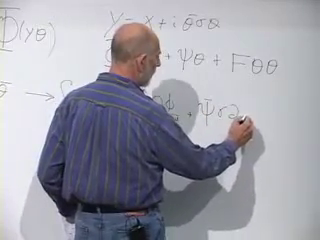
\includegraphics[width=0.76\textwidth]{lecture_09_figure_02.png}\lectureframe{00:27:36.000}\caption{La coordenada quiral y el desarrollo en componentes por encima de los términos del escalar, el fermión y el campo auxiliar.}\end{figure}

\section{Qué selecciona la integral en \texorpdfstring{\(d^2\theta\)}{d2-theta}}

Las interacciones y las masas surgen de una función holomorfa \(W(\Phi)\), el superpotencial:
\begin{equation}
S_W
=
\int d^4x
\left[
\int d^2\theta\,W(\Phi)
+\mathrm{h.c.}
\right].
\label{eq:l9-superpotential-action}
\end{equation}
Una expresión quiral no depende de forma independiente de \(\bar\theta\), de modo que integrarla respecto de las cuatro coordenadas impares daría cero. En cambio, la integral \(d^2\theta\) selecciona su componente \(\theta^2\).

Para ver la combinatoria antes de considerar una función general, sea \(W(\Phi)=\Phi^n\). En
\begin{equation}
(\phi+\sqrt2\,\theta\psi+\theta^2F)^n,
\end{equation}
hay dos maneras de obtener exactamente dos factores \(\theta\). Se puede elegir un solo \(F\theta^2\), o bien elegir dos factores fermiónicos.

\begin{classroomqa}
\audiencequestion{¿Cuántos términos contienen un \(F\theta^2\) elegido y, por lo demás, solo escalares: ¿\(n-1\) o \(n\)? \lecturetimestamp{00:31:33}}
\lecturerresponse{Hay \(n\). Cualquiera de los \(n\) factores puede aportar \(F\theta^2\); los \(n-1\) factores restantes aportan \(\phi\). La contribución es \(nF\phi^{n-1}\).}
\end{classroomqa}

\begin{classroomqa}
\audiencequestion{¿De cuántas maneras pueden dos factores aportar los dos fermiones? \lecturetimestamp{00:32:26}}
\lecturerresponse{Hay \(\binom n2=n(n-1)/2\) elecciones no ordenadas. La contracción de Grassmann fija el término \(\psi\psi\) correspondiente.}
\end{classroomqa}

Así, en la notación de la clase que omite los coeficientes,
\begin{equation}
\int d^2\theta\,\Phi^n+\mathrm{h.c.}
\;\leadsto\;
nF\phi^{n-1}
-\frac{n(n-1)}{2}\phi^{n-2}\psi\psi
+\mathrm{h.c.}
\label{eq:l9-power-extraction}
\end{equation}
El signo menos que se muestra aquí se deriva del desarrollo normalizado estándar y de la convención de Grassmann; al cambiar de convención, pueden cambiar signos aparentes.

\begin{classroomqa}
\audiencequestion{¿Qué ocurrió con el término \(\phi^n\), que no contiene ningún \(\theta\)? \lecturetimestamp{00:33:10}}
\lecturerresponse{Está presente en el producto, pero \(d^2\theta\) lo descarta. La flecha indica que la integración selecciona el coeficiente \(\theta^2\); no expresa una igualdad entre las expresiones completas.}
\end{classroomqa}

\begin{figure}[H]\centering
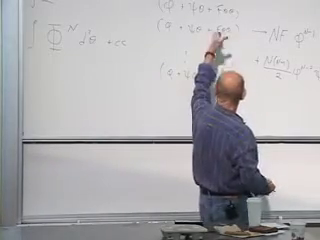
\includegraphics[width=0.82\textwidth]{lecture_09_figure_03.png}\lectureframe{00:33:38.000}\caption{Los factores de supercampo repetidos y la flecha de implicación, que extrae la componente de dos factores \(\theta\) en vez de igualarla a la expresión completa.}\end{figure}

Al sumar potencias con coeficientes arbitrarios, los factores combinatorios se convierten en derivadas:
\begin{equation}
\int d^2\theta\,W(\Phi)+\mathrm{h.c.}
\;\leadsto\;
F W'(\phi)
-\frac12 W''(\phi)\psi\psi
+\mathrm{h.c.}
\label{eq:l9-W-components}
\end{equation}

\begin{classroomqa}
\audiencequestion{¿Por qué el término fermiónico contiene \(\phi^{n-2}\), en vez de \(\phi^{n-1}\)? \lecturetimestamp{00:36:32}}
\lecturerresponse{Dos factores ya han aportado los fermiones, por lo que quedan \(n-2\) factores escalares. El coeficiente es la mitad de la segunda derivada \(W''(\phi)\).}
\end{classroomqa}

El término fermiónico es importante: da una masa cuando \(W''\) es constante y una interacción de Yukawa cuando \(W''\) depende de \(\phi\). Sin embargo, para analizar el vacío, el término auxiliar \(FW'\) proporciona la información inmediata.

\section{Eliminación del campo auxiliar}

Reunamos los términos que contienen \(F\):
\begin{equation}
\mathcal L_F
=
F^\ast F
+F W'(\phi)
+F^\ast \overline{W'(\phi)}.
\label{eq:l9-LF}
\end{equation}
Como no hay término \(\partial_\mu F\), la ecuación completa de Euler--Lagrange
\begin{equation}
\partial_\mu
\frac{\partial\mathcal L}{\partial(\partial_\mu F)}
-
\frac{\partial\mathcal L}{\partial F}
=0
\end{equation}
se reduce inmediatamente a una ecuación algebraica. Al tratar \(F\) y \(F^\ast\) como variables independientes, se obtiene
\begin{align}
\frac{\partial\mathcal L_F}{\partial F}
&=F^\ast+W'(\phi)=0,
&
\frac{\partial\mathcal L_F}{\partial F^\ast}
&=F+\overline{W'(\phi)}=0,
\label{eq:l9-F-eom}
\end{align}
y, por tanto,
\begin{equation}
F^\ast=-W'(\phi),
\qquad
F=-\overline{W'(\phi)}.
\label{eq:l9-F-solution}
\end{equation}

\begin{figure}[H]\centering
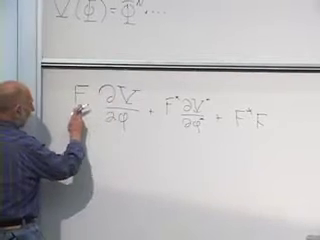
\includegraphics[width=0.82\textwidth]{lecture_09_figure_04.png}\lectureframe{00:39:40.000}\caption{La expresión completa del campo auxiliar y su ecuación de movimiento algebraica, visibles juntas tras despejar la pizarra de los elementos que las ocultaban.}\end{figure}

\begin{classroomqa}
\audiencequestion{¿No debería derivarse respecto de \(\phi\), en vez de respecto del campo conjugado que aparece escrito en la pizarra? \lecturetimestamp{00:41:21}}
\lecturerresponse{Sí. La corrección restablece el par conjugado en la ec.~\eqref{eq:l9-F-eom}: \(F^\ast=-W'(\phi)\) y \(F=-\overline{W'(\phi)}\).}
\end{classroomqa}

Al sustituir en la ec.~\eqref{eq:l9-LF} se obtiene
\begin{equation}
\mathcal L_F\big|_{\mathrm{on\ shell}}
=-|W'(\phi)|^2.
\end{equation}
Como un lagrangiano escalar tiene la forma energía cinética menos energía potencial, el potencial escalar ordinario es
\begin{equation}
\boxed{V(\phi,\phi^\ast)=|W'(\phi)|^2\ge0.}
\label{eq:l9-F-potential}
\end{equation}
Este \(V\) no es el superpotencial. Reservamos \(W\) para la función holomorfa del superspacio y \(V\) para la energía potencial ordinaria.

\subsection{Dos ejemplos inmediatos}

Con las normalizaciones convencionales exactas,
\begin{equation}
\begin{gathered}
W(\Phi)=\frac12m\Phi^2,\\
W'(\phi)=m\phi,
\qquad V=|m|^2|\phi|^2.
\end{gathered}
\label{eq:l9-quadratic-W}
\end{equation}
El mismo término da la masa del fermión
\(-\tfrac12m\psi\psi+\mathrm{h.c.}\), así que las masas del escalar y del fermión coinciden antes de que se rompa la supersimetría.

Para
\begin{equation}
W(\Phi)=\frac{g}{3}\Phi^3,
\end{equation}
se obtiene
\begin{equation}
\begin{gathered}
W'(\phi)=g\phi^2,
\qquad V=|g|^2|\phi|^4,\\
\mathcal L_{\mathrm{Yukawa}}
=-g\phi\psi\psi+\mathrm{h.c.}
\end{gathered}
\label{eq:l9-cubic-W}
\end{equation}
El vértice escalar cuártico describe la dispersión de dos escalares, mientras que el término de Yukawa es su complemento supersimétrico.

\section{Dos tipos de vacío}

El vacío es una configuración de campo constante en un mínimo de \(V\); sus términos con derivadas se anulan. Como la ec.~\eqref{eq:l9-F-potential} es no negativa, hay dos casos posibles.

\subsection{Un mínimo de energía nula}

Si existe algún \(\phi_0\) que satisfaga
\begin{equation}
W'(\phi_0)=0,
\end{equation}
entonces
\begin{equation}
V(\phi_0)=0,
\qquad
\langle F\rangle=0.
\label{eq:l9-unbroken-F}
\end{equation}
El vacío es supersimétrico. Es el análogo de la magnetización nula: ninguna componente auxiliar ha seleccionado una dirección en el superspacio.

\subsection{Un mínimo elevado}

Si las ecuaciones
\begin{equation}
W'(\phi)=0
\label{eq:l9-F-flatness}
\end{equation}
no tienen una solución simultánea en el mínimo, entonces
\begin{equation}
V_{\min}>0,
\qquad
\langle F\rangle\neq0,
\label{eq:l9-broken-F}
\end{equation}
y la supersimetría se rompe espontáneamente. La acción sigue siendo supersimétrica; su estado de menor energía, no.

\begin{figure}[H]\centering
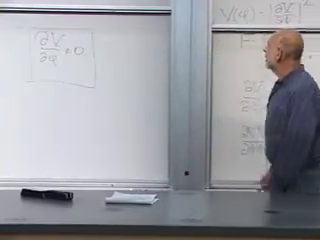
\includegraphics[width=0.88\textwidth]{lecture_09_figure_05.png}\lectureframe{00:52:09.960}\caption{La pizarra muestra el potencial positivo, la ecuación de \(F\) y la condición del vacío, y distingue las ecuaciones simétricas de una solución no simétrica.}\end{figure}

La afirmación sobre el parámetro de orden puede precisarse mediante la transformación del fermión:
\begin{equation}
\delta\psi_\alpha
=
i\sqrt2
(\sigma^\mu\bar\epsilon)_\alpha\partial_\mu\phi
+\sqrt2\,\epsilon_\alpha F.
\label{eq:l9-fermion-transformation}
\end{equation}
En un vacío homogéneo, el término con derivadas se anula. Si
\(\langle F\rangle\neq0\), la supersimetría desplaza el fermión en una cantidad constante distinta de cero, por lo que el vacío no puede ser invariante.\editorialnote{La ecuación~\eqref{eq:l9-fermion-transformation} es la forma estándar en componentes que explicita la afirmación de la clase de que las componentes del supercampo se transforman unas en otras.}

La misma conclusión se obtiene del superálgebra. En el sistema de referencia en reposo,
\begin{equation}
\{Q_\alpha,Q_{\dot\alpha}^\dagger\}
=2\sigma^0_{\alpha\dot\alpha}H.
\end{equation}
Tomar el valor esperado en el vacío expresa su energía como suma de normas de las supercargas actuando sobre él:
\begin{equation}
E_0\ge0,
\qquad
E_0=0
\ \Longleftrightarrow\
Q_\alpha|0\rangle
=Q_{\dot\alpha}^\dagger|0\rangle=0.
\label{eq:l9-algebra-vacuum-energy}
\end{equation}
Así pues, la energía positiva del vacío y la ruptura espontánea de la supersimetría son dos aspectos de una misma afirmación sobre la supersimetría global.

\begin{center}
\begin{tikzpicture}[x=1.2cm,y=1.0cm,>=Latex]
  \draw[->] (-3,0) -- (-0.2,0) node[right] {\(\phi\)};
  \draw[->] (-2.8,-0.15) -- (-2.8,2.1) node[above] {\(V\)};
  \draw[thick,teal!75!black,domain=-2.5:-0.5,samples=60]
    plot (\x,{0.65*(\x+1.5)^2});
  \fill (-1.5,0) circle (2pt);
  \node[below] at (-1.5,0) {\(F=0\)};
  \draw[->] (0.4,0) -- (3.2,0) node[right] {\(\phi\)};
  \draw[->] (0.6,-0.15) -- (0.6,2.1) node[above] {\(V\)};
  \draw[thick,orange!85!black,domain=0.9:2.9,samples=60]
    plot (\x,{0.55*(\x-1.9)^2+0.65});
  \fill (1.9,0.65) circle (2pt);
  \draw[dashed] (0.6,0.65) -- (1.9,0.65);
  \node[below] at (1.9,0.65) {\(F\neq0\)};
\end{tikzpicture}
\end{center}

\editorialnote{Una ilustración mínima es \(W=f\Phi\), para la que \(W'=f\) nunca se anula y \(V=|f|^2\). Este ejemplo de un solo campo tiene una dirección escalar plana; la ruptura estable y realista mediante términos \(F\) suele implementarse con varios campos quirales, como en los sectores ocultos de tipo O'Raifeartaigh.}

\section{Qué produce la ruptura de la supersimetría}

\subsection{Desdoblamiento de masas}

La analogía con el ferromagneto vuelve ahora a los espectros. Un campo magnético interno débil separa los niveles atómicos sin destruir la identidad del átomo. De modo similar, un parámetro de orden que rompe la supersimetría y se comunica débilmente separa los bosones y los fermiones que, de otro modo, pertenecerían a un mismo supermultiplete.

\begin{classroomqa}
\audiencequestion{¿Qué partículas se transforman unas en otras bajo la supersimetría y, por tanto, pierden la degeneración de masas cuando el vacío la rompe? \lecturetimestamp{00:51:40}}
\lecturerresponse{Los bosones y los fermiones. Sus masas ya no tienen por qué seguir siendo iguales cuando el estado deja de respetar la transformación que los relaciona.}
\end{classroomqa}

El desdoblamiento no se produce por \(\langle F\rangle\) de forma aislada; depende de los acoplamientos que transmiten la ruptura a los campos visibles. Si esos acoplamientos son débiles, las partículas visibles siguen siendo reconocibles y los desdoblamientos son pequeños en comparación con las escalas de gran unificación o de Planck. Si fueran fuertes, el análogo sería un átomo tan deformado por un campo magnético enorme que se convertiría en un objeto alargado e irreconocible.

\subsection{El goldstino}

Para un generador bosónico ordinario roto, \(J|0\rangle\) da un estado bosónico de Goldstone. Una supercarga es fermiónica y transforma estados bosónicos en fermiónicos. Como el vacío se considera bosónico, una supercarga rota crea un estado fermiónico de energía cero:
\begin{equation}
Q_\alpha|0\rangle
\sim
|\widetilde G_\alpha,\mathbf k=0\rangle.
\label{eq:l9-goldstino}
\end{equation}
Su continuación propagante es un fermión de Weyl sin masa, el fermión de Goldstone o goldstino.

\begin{classroomqa}
\audiencequestion{Si una transformación supersimétrica no deja invariante el vacío, ¿qué estado nuevo produce? \lecturetimestamp{00:53:24}}
\lecturerresponse{Un fermión sin masa. Se mantiene el patrón del teorema de Goldstone ordinario, pero un generador fermiónico transforma el vacío bosónico en el goldstino.}
\end{classroomqa}

Por tanto, la ruptura espontánea de la supersimetría global tiene dos señales inevitables:
\begin{equation}
\boxed{
V_{\min}>0
\qquad\text{and}\qquad
\text{a massless goldstino}.
}
\label{eq:l9-rigid-breaking-signatures}
\end{equation}

\section{El sector oculto}

Es útil considerar el átomo y el ferromagneto como dos sectores. El ferromagneto desarrolla el parámetro de orden; el átomo solo siente el campo que se le transmite. Cuando el acoplamiento es débil, manipular el átomo apenas excita un magnón y da poco acceso directo al medio magnético. En ese caso, el ferromagneto está oculto, aunque su presencia se infiere a partir de pequeños desdoblamientos espectrales.

La construcción de modelos supersimétricos emplea el mismo lenguaje. Campos adicionales de un sector oculto desarrollan valores esperados no nulos de términos \(F\) o \(D\). Las interacciones denominadas mecanismo de mediación comunican esa ruptura al sector visible y generan masas suaves para las supercompañeras. La transmisión débil explica cómo la teoría visible puede seguir siendo aproximadamente supersimétrica a una escala fundamental mucho más alta y, al mismo tiempo, no mostrar degeneración exacta entre bosones--fermiones a bajas energías.

La construcción no es automática. Hacen falta campos adicionales, un vacío de ruptura estable y un mecanismo de mediación controlado. Por eso, en la clase se describe la ruptura realista de la supersimetría como complicada y algo artificiosa, y no como una consecuencia única e inevitable del modelo mínimo.

\section{La gravedad modifica ambas señales}

\subsection{La energía del vacío se convierte en una fuente}

Sin gravedad, desplazar todas las energías en una constante no cambia los experimentos no gravitatorios. Con gravedad, la densidad de energía del vacío entra en la ecuación de Einstein como constante cosmológica. Un valor positivo de \(V_{\min}\) provoca una expansión acelerada. Si su escala fuera comparable a la escala de física de partículas necesaria para las masas de las supercompañeras, la curvatura resultante sería enormemente mayor que la observada.

\begin{classroomqa}
\audiencequestion{Una vez incluida la gravedad, ¿qué efecto tiene en el universo una energía del vacío positiva y distinta de cero? \lecturetimestamp{01:00:40}}
\lecturerresponse{Actúa como una constante cosmológica y provoca una expansión acelerada. A las escalas habituales de la física de partículas, el efecto sería intolerablemente grande.}
\end{classroomqa}

La supersimetría local, o supergravedad, modifica la fórmula de suma de cuadrados positivos. Para orientarnos, el potencial estándar de términos \(N=1\) \(F\) es
\begin{equation}
\begin{aligned}
V_F={}&e^{K/M_P^2}
\left(
K^{i\bar j}D_iW\,D_{\bar j}\overline W
-\frac{3|W|^2}{M_P^2}
\right),\\
D_iW={}&\partial_iW+\frac{\partial_iK}{M_P^2}W.
\end{aligned}
\label{eq:l9-sugra-potential}
\end{equation}
Debido al término negativo, en principio es posible cancelar parcialmente la energía positiva debida a la ruptura de la supersimetría. El residuo podría ser una constante cosmológica pequeña.

\editorialnote{La clase presenta intencionadamente solo una corrección esquemática y cuestiona explícitamente la ubicación de la masa de Planck. La ecuación~\eqref{eq:l9-sugra-potential} recoge la fórmula convencional para multipletes quirales con potencial de Kähler \(K\); los términos gauge \(D\) aportarían además una contribución no negativa. No explica el diminuto valor observado, que sigue siendo el problema de la constante cosmológica.}

\subsection{El mecanismo de super-Higgs}

El segundo efecto gravitatorio se entiende más fácilmente contando polarizaciones. Una partícula masiva de espín \(j\) tiene \(2j+1\) estados de espín en su sistema de referencia en reposo.

\begin{classroomqa}\audiencequestion{¿Cuántos estados de espín tiene una partícula masiva de espín \(j\)?\lecturetimestamp{01:05:16}}\lecturerresponse{\(2j+1\)En particular, una partícula masiva de espín uno tiene tres estados, mientras que un bosón gauge sin masa solo tiene helicidades \(+1\) y \(-1\).}\end{classroomqa}

La distinción es cinemática. Se puede impulsar una partícula masiva hasta el reposo y luego enviarla en una nueva dirección conservando la orientación de su espín, de modo que deben existir todas las proyecciones. No es posible adelantar a una partícula sin masa ni llevarla al reposo. Por tanto, solo puede tener las dos helicidades extremas.

Para el campo gauge electrodébil,
\begin{equation}
\underbrace{(+1,-1)}_{\text{massless vector}}
+
\underbrace{(0)}_{\text{Goldstone}}
\longrightarrow
\underbrace{(+1,0,-1)}_{\text{massive vector}}.
\label{eq:l9-higgs-count}
\end{equation}

\begin{classroomqa}
\audiencequestion{¿De dónde procede la polarización longitudinal de un \(W\) o un \(Z\) masivo? \lecturetimestamp{01:08:50}}
\lecturerresponse{Del bosón de Goldstone. El campo gauge lo absorbe, completando la representación masiva de espín uno con tres estados.}
\end{classroomqa}

La gravedad tiene un gravitón sin masa de espín dos. Su compañero supersimétrico es el gravitino sin masa de espín \(\tfrac32\).

\begin{classroomqa}
\audiencequestion{¿Cuál es el espín del gravitón y, por tanto, el de su supercompañero? \lecturetimestamp{01:10:24}}
\lecturerresponse{El gravitón tiene espín \(2\); su compañero fermiónico difiere en un medio y tiene espín \(3/2\).}
\end{classroomqa}

Un gravitino sin masa tiene helicidades \(\pm\tfrac32\), mientras que uno masivo también debe tener \(\pm\tfrac12\). El goldstino aporta precisamente esos estados que faltan:
\begin{equation}
\begin{gathered}
\underbrace{\left(+\frac32,-\frac32\right)}_{\text{massless gravitino}}
\oplus
\underbrace{\left(+\frac12,-\frac12\right)}_{\text{goldstino}}\\
\Downarrow\\
\underbrace{\left(+\frac32,+\frac12,-\frac12,-\frac32\right)}_{\text{massive gravitino}}.
\end{gathered}
\label{eq:l9-super-higgs}
\end{equation}
Este es el mecanismo de super-Higgs. Cuando la supersimetría es local, el goldstino es absorbido y deja de aparecer como una partícula independiente sin masa. El gravitino resultante interactúa gravitatoriamente y, por ello, es difícil de producir.

\section{Cambio de tema: ¿por qué \texorpdfstring{\(SU(5)\)}{SU(5)}?}

Ahora el formalismo de la supersimetría da paso a la gran unificación. El grupo gauge del modelo estándar es
\begin{equation}
G_{\mathrm{SM}}
=SU(3)_c\times SU(2)_L\times U(1)_Y.
\label{eq:l9-sm-group}
\end{equation}
Sus tres factores organizan por separado el color, el isoespín débil y la hipercarga débil. La pregunta sobre la unificación es si este producto es el subgrupo residual de un único grupo simple mayor, de modo que los multipletes de partículas y las fuerzas gauge aparentemente separados sean partes de una sola estructura. El candidato mínimo que se desarrolla aquí es \(SU(5)\).

\subsection{Elementos y generadores del grupo}

Para \(U\in SU(N)\),
\begin{equation}
U^\dagger U=\mathbf1,
\qquad
\det U=1.
\label{eq:l9-SUN-def}
\end{equation}
La primera condición expresa la unitariedad; la segunda es lo que significa ser especial. Escribamos un elemento infinitesimal como
\begin{equation}
U=\mathbf1+i\epsilon G+\mathcal O(\epsilon^2).
\label{eq:l9-infinitesimal-U}
\end{equation}
La unitariedad exige
\begin{equation}
G^\dagger=G,
\end{equation}
y
\begin{equation}
\det e^{i\epsilon G}
=e^{i\epsilon\operatorname{tr}G}=1
\end{equation}
exige
\begin{equation}
\operatorname{tr}G=0.
\end{equation}
Así pues, los generadores son matrices hermíticas sin traza.

Una matriz hermítica \(N\times N\) contiene \(N^2\) parámetros reales: \(N\) entradas diagonales reales y \(N(N-1)/2\) entradas complejas fuera de la diagonal. La condición de traza nula elimina uno. Por tanto,
\begin{equation}
\dim SU(N)=N^2-1,
\qquad
\dim SU(5)=24.
\label{eq:l9-SU5-dimension}
\end{equation}
A modo de comparación, \(SU(2)\) tiene tres generadores de Pauli y \(SU(3)\) tiene ocho generadores de color.

\section{Los bloques del modelo estándar dentro de \texorpdfstring{\(SU(5)\)}{SU(5)}}

Dividamos el espacio de cinco dimensiones en un bloque débil bidimensional y un bloque de color tridimensional:
\begin{equation}
\mathbf5=\mathbf2\oplus\mathbf3.
\end{equation}
Los generadores embebidos tienen las formas
\begin{align}
T^a_L
&=
\begin{pmatrix}
\tfrac12\tau^a&0\\
0&0_{3\times3}
\end{pmatrix},
&& a=1,2,3,
\label{eq:l9-SU2-block}\\
T^A_c
&=
\begin{pmatrix}
0_{2\times2}&0\\
0&\tfrac12\lambda^A
\end{pmatrix},
&& A=1,\ldots,8.
\label{eq:l9-SU3-block}
\end{align}
Las matrices de Pauli \(\tau^a\) generan el grupo débil \(SU(2)\); las matrices de Gell-Mann \(\lambda^A\) generan el grupo de color \(SU(3)\). Como los bloques no se superponen, los dos subgrupos conmutan.

Un generador diagonal adicional es proporcional a la identidad dentro de cada bloque y, por tanto, conmuta con ambos. En la representación fundamental, una convención conveniente para la hipercarga duplicada es
\begin{equation}
T_Y^{(\mathbf5)}=
\operatorname{diag}
\left(
1,1,-\frac23,-\frac23,-\frac23
\right).
\label{eq:l9-hypercharge-generator}
\end{equation}
Su traza se anula:
\begin{equation}
1+1-3\left(\frac23\right)=0.
\end{equation}
La representación conjugada de materia tiene los valores propios opuestos,
\begin{equation}
Y_{\overline{\mathbf5}}
=
\operatorname{diag}
\left(
-1,-1,\frac23,\frac23,\frac23
\right),
\label{eq:l9-fivebar-hypercharge}
\end{equation}
que son los valores escritos para la columna de materia en la clase. El signo global y la normalización son convencionales; estas entradas emplean la convención del modelo estándar
\begin{equation}
Q=T_3+\frac{Y}{2}.
\label{eq:l9-charge}
\end{equation}
Las ecuaciones~\eqref{eq:l9-SU2-block}--\eqref{eq:l9-hypercharge-generator} muestran
\begin{equation}
SU(3)_c\times SU(2)_L\times U(1)_Y
\subset SU(5).
\end{equation}

Los tres generadores débiles, los ocho generadores de color y el generador de hipercarga suman \(12\) de los \(24\) generadores de \(SU(5)\).\editorialnote{Los otros doce ocupan los bloques no diagonales \(2\times3\) y \(3\times2\). Sus bosones de gauge convierten componentes de tipo quark en componentes de tipo leptón, y viceversa; este es el origen estructural de las interacciones que cambian el número bariónico y leptónico, desarrolladas en la continuación.}

\begin{classroomqa}
\audiencequestion{¿Qué partículas de gauge corresponden a los generadores familiares del subgrupo? \lecturetimestamp{01:31:05}}
\lecturerresponse{Los ocho generadores de \(SU(3)\) dan lugar a los ocho gluones. Los tres generadores de \(SU(2)\) dan lugar a los campos de gauge débiles, que, tras la mezcla electrodébil, se convierten en \(W^\pm\) y en parte del sistema \(Z\)-fotón; el campo \(U(1)\) aporta la otra combinación neutra.}
\end{classroomqa}

\section{Una familia expresada en términos de campos izquierdos}

Centrémonos en la primera generación; el mismo patrón se repite para las generaciones del muón, el quark charm y el quark strange, y del tau, el quark top y el quark bottom. Lo más sencillo es contar cada campo de Weyl independiente como un campo izquierdo. Las partículas derechas se representan mediante sus campos conjugados de carga izquierdos:
\begin{equation}
Q_L=(u_L,d_L),\quad
L_L=(\nu_{eL},e_L),\quad
u^c_L,\quad d^c_L,\quad e^c_L.
\end{equation}
Sus multiplicidades son
\begin{equation}
\underbrace{6}_{Q_L}
+
\underbrace{2}_{L_L}
+
\underbrace{3}_{u^c_L}
+
\underbrace{3}_{d^c_L}
+
\underbrace{1}_{e^c_L}
=15.
\label{eq:l9-fifteen-fields}
\end{equation}

\editorialnote{El Modelo Estándar mínimo no contiene ningún campo de Weyl independiente de neutrino derecho, así que el recuento es \(15\). Este recuento, por sí solo, no afirma que el neutrino sea una partícula de Majorana. Al añadir un singlete \(\nu^c_L\), se obtienen \(16\) campos y se apunta de forma natural a \(SO(10)\), más allá de la construcción \(SU(5)\) que consideramos aquí.}

El multiplete de cinco dimensiones debe situar en las dos primeras posiciones los componentes de doblete débil sin color, y en las tres últimas, los singletes débiles con color.

\begin{classroomqa}
\audiencequestion{¿La columna propuesta contiene seis campos en vez de cinco? \lecturetimestamp{01:36:14}}
\lecturerresponse{No. Se tacha el quark up escrito en el primer intento. La columna contiene el neutrino, el electrón y tres copias de color del antiquark down: cinco componentes en total.}
\end{classroomqa}

Esto da
\begin{equation}
\overline{\mathbf5}
=
\begin{pmatrix}
\nu_{eL}\\
e_L\\
d^c_{rL}\\
d^c_{gL}\\
d^c_{bL}
\end{pmatrix}.
\label{eq:l9-fivebar}
\end{equation}
\editorialnote{La clase la denomina inicialmente, sin más, un multiplete de cinco dimensiones. En la notación estándar en la que todos los campos son izquierdos, las asignaciones de color e hipercarga la identifican como la representación conjugada \(\overline{\mathbf5}\) de \(SU(5)\).}
Los dos primeros componentes se transforman bajo \(SU(2)_L\), pero no llevan color. Los tres últimos se transforman como un antitriplete de color, pero son singletes débiles.

\begin{classroomqa}
\audiencequestion{Una vez que todos los campos se expresan como izquierdos, ¿qué quarks llevan color, pero no tienen número cuántico débil \(SU(2)_L\)? \lecturetimestamp{01:40:13}}
\lecturerresponse{Los conjugados de carga de los quarks derechos. Para este multiplete de cinco componentes, la condición de carga selecciona los tres campos de antiquark down \(d^c_{r,g,b}\).}
\end{classroomqa}

Las cargas eléctricas de la ecuación~\eqref{eq:l9-fivebar} suman cero:
\begin{equation}
0-1+\frac13+\frac13+\frac13=0.
\label{eq:l9-fivebar-charge-sum}
\end{equation}
Esto es necesario porque el operador de carga eléctrica es una combinación sin traza de generadores de \(SU(5)\).

\begin{classroomqa}
\audiencequestion{¿Por qué ocupan los tres espacios de color los antiquarks down y no los antiquarks up? \lecturetimestamp{01:43:38}}
\lecturerresponse{El neutrino y el electrón aportan una carga total de \(-1\). Los tres colores del antiquark down aportan \(+1\), con lo que la traza es cero. Tres campos de antiquark up darían una carga total incorrecta.}
\end{classroomqa}

Los diez campos izquierdos restantes son
\begin{equation}
Q_L\;(6)
\oplus
u^c_L\;(3)
\oplus
e^c_L\;(1),
\end{equation}
y encajan exactamente en la representación antisimétrica de rango dos
\begin{equation}
\mathbf{10}\cong\wedge^2\mathbf5,
\qquad
\dim\wedge^2\mathbf5=\binom52=10.
\label{eq:l9-ten-preview}
\end{equation}
La siguiente clase se ocupará de su ubicación explícita. El ajuste numérico
\begin{equation}
\overline{\mathbf5}\oplus\mathbf{10}
\end{equation}
en cada familia del Modelo Estándar constituye la primera evidencia notable de que la idea de \(SU(5)\) va más allá de un cambio de nombres arbitrario.

\begin{classroomqa}
\audiencequestion{Si el cinco y el diez son representaciones distintas, ¿significa eso que sus partículas no pueden interactuar? \lecturetimestamp{01:46:14}}
\lecturerresponse{No. Una transformación del grupo actúa dentro de cada representación irreducible, de modo que no rota directamente un elemento del cinco hasta uno del diez. Sin embargo, los dos conjuntos pueden interactuar emitiendo y absorbiendo bosones de gauge comunes, y los acoplamientos de Higgs también pueden conectar sus campos.}
\end{classroomqa}

\section{Perspectiva}

La clase ha seguido un mismo patrón a través de escalas muy distintas. La invariancia rotacional hace que los niveles atómicos sean degenerados; un campo magnético los desdobla. Un ferromagneto produce ese campo sin dejar de respetar la simetría de las leyes subyacentes, y sus magnones sin brecha revelan que la asimetría reside en el vacío. En una teoría supersimétrica quiral, el valor esperado del campo auxiliar desempeña el papel del parámetro de orden:
\begin{equation}
\begin{aligned}
\langle F\rangle=0
&\quad\Longleftrightarrow\quad
\text{unbroken supersymmetry},\\
\langle F\rangle\neq0
&\quad\Longrightarrow\quad
\text{spontaneous breaking}.
\end{aligned}
\end{equation}
En la supersimetría rígida, el vacío roto tiene energía positiva, desdobla los supermultipletes y genera un goldstino. La mediación débil motiva la introducción de un sector oculto; la gravedad convierte la energía del vacío en un problema cosmológico y absorbe el goldstino en un gravitino masivo.

La construcción de cierre con \(SU(5)\) plantea una pregunta nueva en lugar de resolverla. Los generadores hermíticos sin traza de \(5\times5\) contienen los bloques del Modelo Estándar, y los cinco primeros campos de materia encajan exactamente como \((\nu_e,e^-,d^c_r,d^c_g,d^c_b)\). Los diez restantes esperan en la representación antisimétrica. Ahí, en ese encaje aún incompleto, es donde comienza propiamente la gran unificación.

\chapter{Los multipletes de \texorpdfstring{\(SU(5)\)}{SU(5)}, los bosones gauge leptoquarks y la desintegración del protón}

\lectureoverview{La gran unificación se vuelve concreta cuando el grupo del Modelo Estándar se incorpora en \(SU(5)\). Para entender qué significa esta afirmación, primero desarrollamos la teoría de representaciones necesaria: la representación definitoria \(N\), su conjugada \(\overline N\), los productos tensoriales, los tensores simétricos y antisimétricos, y la representación adjunta. Una familia del Modelo Estándar queda entonces reunida en la combinación, inesperadamente económica, \(\overline{\mathbf 5}\oplus\mathbf{10}\). La misma simetría que hace bella esta organización también exige bosones gauge coloreados que convierten quarks en leptones. Su intercambio permite la desintegración del protón y obliga a situar la escala de unificación cerca de \(10^{15}\)--\(10^{16}\,\mathrm{GeV}\). Los acoplamientos gauge que evolucionan con la escala apuntan a una escala similar; la supersimetría reaparece al final porque hace mucho más precisa su coincidencia numérica.}

\section{¿Por qué empezar con las representaciones de grupo?}

Se han propuesto muchas teorías de gran unificación. En lugar de repasarlas, analizaremos un ejemplo y plantearemos tres preguntas: qué lo hace funcionar, qué nuevas partículas exige y dónde lo pone en peligro la experimentación. El grupo es \(SU(5)\), y su característica estructural definitoria es la inclusión
\begin{equation}
SU(3)_c\times SU(2)_L\times U(1)_Y
\subset SU(5).
\label{eq:l10-sm-embedding}
\end{equation}
Aquí \(SU(3)_c\) actúa sobre el color, \(SU(2)_L\) sobre el isospín débil y \(U(1)_Y\) sobre la hipercarga.

La supersimetría no es una premisa de esta construcción. Ni la supersimetría implica lógicamente la gran unificación ni ocurre lo contrario. La conexión entre ambas en esta lección es numérica: al incluir el espectro de supercompañeras en el cálculo del grupo de renormalización, los tres acoplamientos gauge se aproximan con mayor precisión a un valor común.

Las partículas que una simetría mezcla entre sí forman una representación del grupo de simetría. Por lo tanto, para clasificar los multipletes de partículas unificadas primero necesitamos algo de teoría de representaciones.

\subsection{El conocido ejemplo de \texorpdfstring{\(SU(2)\)}{SU(2)}}

El \(SU(2)\) asociado al momento angular ordinario está estrechamente relacionado con las rotaciones del espacio tridimensional. Más precisamente, \(SU(2)\) es el recubrimiento doble de \(SO(3)\). Sus representaciones irreducibles se etiquetan mediante
\begin{equation}
j=0,\frac12,1,\frac32,\ldots,
\qquad
\dim(j)=2j+1.
\label{eq:l10-su2-spins}
\end{equation}
Así, un escalar es un singlete, una partícula de espín \(\tfrac12\) es un doblete y una partícula de espín uno es un triplete. El grupo débil \(SU(2)_L\) es una simetría física distinta, aunque su teoría de grupos abstracta sea la misma.

\section{La representación definitoria y su conjugada}

Para \(SU(N)\), la representación definitoria es el espacio de columnas complejas con \(N\) componentes,
\begin{equation}
\psi=
\begin{pmatrix}
\psi_1\\
\psi_2\\
\vdots\\
\psi_N
\end{pmatrix},
\qquad
\psi'_i=U_i{}^j\psi_j,
\qquad
U\in SU(N).
\label{eq:l10-defining}
\end{equation}
Se denomina representación definitoria o, simplemente, \(\mathbf N\). Las matrices \(U\) son de tamaño \(N\times N\) y el espacio vectorial sobre el que actúan tiene dimensión \(N\).

La conjugación compleja da otra representación de dimensión \(N\),
\begin{equation}
\psi_i^*\longmapsto U_i{}^{j*}\psi_j^*,
\label{eq:l10-conjugate}
\end{equation}
denotada por \(\overline{\mathbf N}\). Para \(N>2\), las representaciones definitoria y conjugada no son equivalentes. Se puede intercambiar cuál se denomina representación de la partícula y cuál representación de la antipartícula, pero, una vez elegida una convención, hay que mantenerla.

\begin{classroomqa}
\audiencequestion{¿El \(N\) de \(SU(N)\) depende de que \(N\) sea par o impar, y se refiere a las matrices? \lecturetimestamp{00:07:33}}
\lecturerresponse{Aquí no hay ninguna restricción de paridad par--impar. \(N\) es el tamaño de las matrices definitorias y también la dimensión de su representación definitoria. Tanto \(\mathbf N\) como \(\overline{\mathbf N}\) tienen esa dimensión.}
\end{classroomqa}

La antipartícula de una antipartícula es la partícula original. Por eso, intercambiar los nombres \(\mathbf N\) y \(\overline{\mathbf N}\) cambia la convención, no la física.

\section{Productos tensoriales e irreducibilidad}

Supongamos que un objeto puede ocupar \(N\) estados internos y que otro objeto puede ocupar independientemente la misma cantidad. Si ignoramos la posición, el momento, el espín y todos los números cuánticos excepto esta etiqueta de \(SU(N)\), el par tiene
\begin{equation}
N\times N=N^2
\label{eq:l10-product-count}
\end{equation}
estados. Si el primer objeto está en el estado \(\psi_i\) y el segundo en el estado \(\phi_j\), su producto se puede escribir como
\begin{equation}
\Psi_{ij}=\psi_i\phi_j,
\qquad
\Psi'_{ij}=U_i{}^kU_j{}^\ell\Psi_{k\ell}.
\label{eq:l10-tensor-transform}
\end{equation}
Este es el producto tensorial \(\mathbf N\otimes\mathbf N\).

\begin{classroomqa}
\audiencequestion{¿Por qué el resultado es \(N^2\) en lugar de \(N^2-1\), y permitir que ambas partículas tengan la misma etiqueta interna viola el principio de exclusión? \lecturetimestamp{00:10:22}}
\lecturerresponse{Aquí los dos lugares son distinguibles: un objeto permanece fijo en una posición y el otro, en otra. El principio de Pauli impone restricciones al estado cuántico completo, incluida la posición. No elimina ninguna de estas \(N^2\) combinaciones de etiquetas internas. El número \(N^2-1\) aparecerá más adelante debido a una condición de traza nula en un producto distinto.}
\end{classroomqa}

En general, la representación producto de dimensión \(N^2\) es reducible. Una representación es reducible cuando contiene un subespacio propio que el grupo transforma en sí mismo. Se pueden separar los subespacios invariantes y tratarlos como representaciones más pequeñas; si no existe tal subespacio propio, la representación es irreducible.

\subsection{Tensores simétricos y antisimétricos}

Todo tensor de dos índices se descompone de manera única en
\begin{align}
\Psi_{ij}
&=\Psi^{(S)}_{ij}+\Psi^{(A)}_{ij},\\
\Psi^{(S)}_{ij}
&=\frac12(\Psi_{ij}+\Psi_{ji}),\\
\Psi^{(A)}_{ij}
&=\frac12(\Psi_{ij}-\Psi_{ji}).
\label{eq:l10-sym-anti}
\end{align}
Las dos partes satisfacen
\begin{equation}
\Psi^{(S)}_{ij}=\Psi^{(S)}_{ji},
\qquad
\Psi^{(A)}_{ij}=-\Psi^{(A)}_{ji}.
\end{equation}
La ecuación~\eqref{eq:l10-tensor-transform} conserva cada condición, por lo que las transformaciones del grupo nunca mezclan los sectores simétrico y antisimétrico.

\editorialnote{La lección deja como ejercicio el recuento general. Las dimensiones de los sectores simétrico y antisimétrico son \(N(N+1)/2\) y \(N(N-1)/2\), respectivamente, y su suma es \(N^2\).}

\begin{figure}[htbp]
\centering
\includegraphics[width=0.78\textwidth]{lecture_10_figure_02.png}
\lectureframe{00:17:57.500}
\caption{Descomposición completa en la pizarra de dos estados de espín \(\tfrac12\): tres estados simétricos y uno antisimétrico.}
\label{fig:l10-spin-decomposition}
\end{figure}

Para el doblete definitorio de \(SU(2)\),
\begin{equation}
\mathbf2\otimes\mathbf2=\mathbf3_S\oplus\mathbf1_A.
\label{eq:l10-two-two}
\end{equation}
Si escribimos los dos estados de la base como \(u\) y \(d\), el triplete simétrico es
\begin{align}
\ket{1,1}&=\ket{uu},\\
\ket{1,0}&=\frac{1}{\sqrt2}\bigl(\ket{ud}+\ket{du}\bigr),\\
\ket{1,-1}&=\ket{dd},
\end{align}
mientras que el singlete antisimétrico es
\begin{equation}
\ket{0,0}
=\frac{1}{\sqrt2}\bigl(\ket{ud}-\ket{du}\bigr).
\end{equation}
Esta es la conocida suma de dos momentos angulares de espín \(\tfrac12\): los cuatro estados iniciales se reorganizan en espín uno y espín cero.

\section{Una partícula y una antipartícula: la representación adjunta}

Ahora combinemos la representación definitoria con su conjugada. El producto sigue teniendo \(N^2\) componentes, pero se transforma como una matriz:
\begin{equation}
M_i{}^j\in\mathbf N\otimes\overline{\mathbf N},
\qquad
M\longmapsto U M U^\dagger.
\label{eq:l10-matrix-transform}
\end{equation}
A diferencia de \(\mathbf N\otimes\mathbf N\), no existe una simetría de intercambio significativa entre un índice fundamental y uno antifundamental. La descomposición natural es, en cambio,
\begin{equation}
M
=
\frac{\operatorname{tr}M}{N}\,\mathbf1_N
+
\left(M-\frac{\operatorname{tr}M}{N}\,\mathbf1_N\right).
\label{eq:l10-trace-split}
\end{equation}
El primer término es un singlete y la parte sin traza es la representación adjunta:
\begin{equation}
\mathbf N\otimes\overline{\mathbf N}
=\mathbf1\oplus\mathbf{Adj},
\qquad
\dim\mathbf{Adj}=N^2-1.
\label{eq:l10-adjoint}
\end{equation}

\begin{figure}[htbp]
\centering
\includegraphics[width=0.67\textwidth]{lecture_10_figure_04.png}
\lectureframe{00:23:47.500}
\caption{Conclusión en la pizarra para \(\mathbf N\otimes\overline{\mathbf N}\): sus \(N^2-1\) componentes sin traza forman la representación adjunta.}
\label{fig:l10-adjoint}
\end{figure}

Para \(SU(3)\), esto da el octete conocido,
\begin{equation}
\mathbf3\otimes\overline{\mathbf3}
=\mathbf8\oplus\mathbf1,
\end{equation}
y los ocho gluones se transforman según la representación adjunta. Para \(SU(2)\), la representación adjunta tiene dimensión tres y se transforma como el espín uno.

\section{Una familia del Modelo Estándar}

Se observan tres generaciones, pero \(SU(5)\) repite la misma construcción por separado para cada una. No explica por qué hay tres copias. Por eso nos centramos en la primera generación.

Todos los campos se escribirán como campos de Weyl levógiros. Un fermión dextrógiro se representa mediante su campo conjugado de carga levógiro:
\begin{equation}
u^c_L,\qquad d^c_L,\qquad e^c_L.
\label{eq:l10-left-handed-bookkeeping}
\end{equation}
El superíndice \(c\) denota conjugación de carga; por ejemplo, \(d^c_L\) es un campo de antiquark down levógiro con carga eléctrica \(+\tfrac13\).

En la notación estándar de \(SU(5)\), cinco de los quince campos levógiros caben en
\begin{equation}
\overline{\mathbf5}
=
\begin{pmatrix}
\nu_{eL}\\
e_L\\
d^c_{rL}\\
d^c_{gL}\\
d^c_{bL}
\end{pmatrix}.
\label{eq:l10-fivebar}
\end{equation}
Se ha elegido el orden de modo que aparezca primero un bloque bidimensional débil y después uno tridimensional de color. Las transformaciones débiles mezclan las dos primeras entradas, las transformaciones de color mezclan las tres últimas y los generadores \(SU(5)\) no diagonales conectan ambos bloques.

\editorialnote{La lección llama \(\mathbf5\) a la columna de la ecuación~\eqref{eq:l10-fivebar} y más adelante llama \(\overline{\mathbf{10}}\) al multiplete antisimétrico. Esta es la convención conjugada globalmente. Usamos la convención estándar moderna \(\overline{\mathbf5}\oplus\mathbf{10}\); conjugar todas las representaciones reproduce las etiquetas de la lección sin cambiar su física.}

El inventario mínimo completo de la primera generación es
\begin{equation}
\begin{gathered}
\underbrace{Q_L=(u_L,d_L)}_{6}
\oplus
\underbrace{L_L=(\nu_{eL},e_L)}_{2},\\
\underbrace{u^c_L}_{3}
\oplus
\underbrace{d^c_L}_{3}
\oplus
\underbrace{e^c_L}_{1},\\
6+2+3+3+1=15.
\end{gathered}
\label{eq:l10-fifteen}
\end{equation}
El Modelo Estándar mínimo no incluye un \(\nu^c_L\) independiente, por lo que no da una masa de neutrino renormalizable. Las oscilaciones de neutrinos muestran que esta descripción mínima es incompleta: la naturaleza tiene masas de neutrino pequeñas, pero distintas de cero, y se necesita una extensión.

\begin{classroomqa}
\audiencequestion{Cuando una masa fermiónica transforma un estado levógiro en uno dextrógiro, ¿también convierte la partícula en su antipartícula? \lecturetimestamp{00:34:00}}
\lecturerresponse{No. La masa del electrón conecta un electrón levógiro con un electrón dextrógiro de la misma carga eléctrica. En la notación con todos los campos levógiros, el segundo campo se representa mediante \(e^c_L\), pero la partícula de cuatro componentes sigue siendo un electrón. Solo un campo neutro puede tener una masa de Majorana que identifique la partícula con la antipartícula.}
\end{classroomqa}

\section{Bosones gauge visibles en el multiplete de cinco}

A cada generador de una simetría gauge le corresponde un campo gauge. En ~\eqref{eq:l10-fivebar} ya se reconocen las transiciones conocidas:
\begin{itemize}
\item los campos gauge débiles actúan entre \(\nu_{eL}\) y \(e_L\);
\item los gluones actúan entre los tres colores de \(d^c_L\);
\item los generadores neutros actúan diagonalmente;
\item los nuevos generadores no diagonales convierten una entrada leptónica en una entrada coloreada, o viceversa.
\end{itemize}

Se puede imaginar que el gluón lleva números cuánticos de color de quark--antiquark. La lección emplea el mnemónico habitual de las líneas de mundo: si seguimos hacia atrás una antiquark saliente a través del vértice de emisión, parece un quark que avanza. Por tanto, el campo emitido lleva los números cuánticos de un par quark--antiquark. En el lenguaje de las representaciones, esta es precisamente la parte sin traza de \(\mathbf3\otimes\overline{\mathbf3}\).

Para \(SU(5)\),
\begin{equation}
\dim\mathbf{Adj}_{SU(5)}=5^2-1=24.
\end{equation}
La descomposición de estos campos gauge bajo el subgrupo del Modelo Estándar es
\begin{equation}
\mathbf{24}
=
(\mathbf8,\mathbf1)_0
\oplus(\mathbf1,\mathbf3)_0
\oplus(\mathbf1,\mathbf1)_0
\oplus(\mathbf3,\mathbf2)_{-5/6}
\oplus(\overline{\mathbf3},\mathbf2)_{5/6},
\label{eq:l10-adjoint-sm}
\end{equation}
donde el par ordenado denota \(SU(3)_c\times SU(2)_L\) y el subíndice es la hipercarga.

\editorialnote{La ecuación~\eqref{eq:l10-adjoint-sm} hace explícita la estructura en bloques dibujada en la lección. Los tres primeros términos contienen los campos gauge conocidos del color y de la interacción electrodébil. Los dos últimos términos son los doce grados de libertad reales que convencionalmente se denominan bosones \(X\) y \(Y\).}

\begin{figure}[htbp]
\centering
\begin{tikzpicture}[x=1.05cm,y=0.82cm]
  \draw[thick] (0,0) rectangle (5,5);
  \draw[thick] (2,0) -- (2,5);
  \draw[thick] (0,3) -- (5,3);
  \fill[blue!9] (0,3) rectangle (2,5);
  \fill[orange!10] (2,0) rectangle (5,3);
  \fill[teal!9] (2,3) rectangle (5,5);
  \fill[teal!9] (0,0) rectangle (2,3);
  \node[align=center] at (1,4) {weak and\\neutral fields};
  \node[align=center] at (3.5,1.5) {gluons and\\neutral field};
  \node[align=center] at (3.5,4) {\(X,Y\)};
  \node[align=center] at (1,1.5) {\(\overline X,\overline Y\)};
  \node[above] at (1,5) {\(2\)};
  \node[above] at (3.5,5) {\(3\)};
\end{tikzpicture}
\caption{La estructura en bloques \(2\oplus3\) del campo gauge de \(SU(5)\). Los bloques no diagonales conectan leptones y campos coloreados.}
\label{fig:l10-gauge-blocks}
\end{figure}

Con \(Q=T_3+Y\), el doblete débil coloreado de ~\eqref{eq:l10-adjoint-sm} tiene cargas \(-\tfrac13\) y \(-\tfrac43\); su conjugado tiene cargas \(+\tfrac13\) y \(+\tfrac43\). La lección llama \(X\) y \(Y\) a estas partículas, pero se abstiene explícitamente de asignar cada nombre a una carga determinada. La transición y la carga son el contenido invariante.

\begin{classroomqa}
\audiencequestion{¿Hay tres versiones de cada nuevo bosón gauge \(X\) o \(Y\)? \lecturetimestamp{00:41:28}}
\lecturerresponse{Sí. Una transición conecta una entrada de quark coloreada con una entrada leptónica sin color, por lo que el bosón intercambiado debe llevar el color que falta. Los campos \(X/Y\) forman tripletes de color y pueden emitir o absorber gluones.}
\end{classroomqa}

No se observan partículas coloreadas como estados asintóticos aislados. Los nuevos bosones gauge deben desintegrarse o hadronizarse en combinaciones neutras de color, igual que los quarks.

\section{Por qué el multiplete contiene antiquarks down}

Los generadores de \(SU(N)\) son matrices hermíticas sin traza. Para ver la relación con la palabra «especial», escribamos un elemento infinitesimal del grupo como
\begin{equation}
U(\epsilon)=e^{i\epsilon T}.
\end{equation}
La unitariedad da \(T^\dagger=T\), mientras que
\begin{equation}
1=\det U=e^{i\epsilon\operatorname{tr}T}
\end{equation}
para \(\epsilon\) arbitrario da
\begin{equation}
\operatorname{tr}T=0.
\label{eq:l10-traceless-generator}
\end{equation}

La carga eléctrica es una combinación lineal de generadores. Sobre la columna de materia de ~\eqref{eq:l10-fivebar}, actúa como
\begin{equation}
Q_{\overline5}
=
\operatorname{diag}
\left(0,-1,\frac13,\frac13,\frac13\right),
\qquad
\operatorname{tr}Q_{\overline5}=0.
\label{eq:l10-charge-fivebar}
\end{equation}
Por tanto,
\begin{equation}
0-1+3\left(\frac13\right)=0.
\end{equation}
Si se reemplazaran los campos de antiquark down por campos de quark down, se obtendría, en cambio,
\begin{equation}
0-1+3\left(-\frac13\right)=-2,
\end{equation}
que no puede ser la traza de un generador de \(SU(5)\). Así, la aparentemente extraña asignación de antiquarks down viene impuesta por la estructura del grupo.

\section{Los diez fermiones restantes}

Los otros diez campos surgen de un tensor antisimétrico de dos índices. En la convención estándar, este es la parte antisimétrica de
\begin{equation}
\mathbf5\otimes\mathbf5
=\mathbf{15}_S\oplus\mathbf{10}_A.
\label{eq:l10-five-five}
\end{equation}
La lección lo construye escribiendo temporalmente los números cuánticos conjugados
\begin{equation}
\chi=
\begin{pmatrix}
\nu^c\\
e^c\\
d_r\\
d_g\\
d_b
\end{pmatrix}.
\label{eq:l10-aux-five}
\end{equation}
Se trata de un recurso contable para formar productos tensoriales de representaciones, no de afirmar que exista un segundo multiplete físico de cinco partículas compuestas.

Sea
\begin{equation}
\Psi^{ij}=-\Psi^{ji},
\qquad
i,j=1,\ldots,5.
\label{eq:l10-antisym-ten}
\end{equation}
Todas las entradas diagonales son nulas y las entradas del triángulo inferior quedan determinadas por las del triángulo superior. Por tanto,
\begin{equation}
\dim\mathbf{10}
=\binom52
=\frac{5\cdot4}{2}
=10.
\label{eq:l10-ten-count}
\end{equation}

La carga eléctrica de una entrada es la suma de las cargas de fila y columna en ~\eqref{eq:l10-aux-five}. De ahí se obtiene inmediatamente \(e^c\) en la posición débil--débil, los quarks down y up en los bloques débil--color, y los campos de anti-up en el bloque color--color.

\begin{classroomqa}
\audiencequestion{Al combinar las etiquetas del positrón y del quark down, ¿debería la entrada resultante ser un bosón \(X\)? \lecturetimestamp{00:53:08}}
\lecturerresponse{No. En esta etapa construimos la representación de los fermiones, no la representación adjunta de los bosones gauge. Las cargas se suman como \(1-\tfrac13=\tfrac23\), así que la entrada tiene los números cuánticos de un quark up.}
\end{classroomqa}

Una elección coherente de los signos de color es
\begin{equation}
\Psi^{ij}=
\begin{pmatrix}
0 & e^c & d_r & d_g & d_b\\
-e^c & 0 & u_r & u_g & u_b\\
-d_r & -u_r & 0 & u_b^c & -u_g^c\\
-d_g & -u_g & -u_b^c & 0 & u_r^c\\
-d_b & -u_b & u_g^c & -u_r^c & 0
\end{pmatrix}.
\label{eq:l10-ten-matrix}
\end{equation}
Cambiar las fases de los campos modifica algunos signos mostrados, pero no la representación ni el contenido de partículas.

\begin{figure}[htbp]
\centering
\includegraphics[width=0.83\textwidth]{lecture_10_figure_05.png}
\lectureframe{00:59:17.500}
\caption{La matriz antisimétrica de materia \(2\oplus3\), sin obstrucciones, una vez comprobadas en clase las entradas y las etiquetas de color.}
\label{fig:l10-ten-board}
\end{figure}

\begin{classroomqa}
\audiencequestion{¿Hay que escribir la representación de dimensión diez como una matriz o se puede escribir como una columna? \lecturetimestamp{00:56:24}}
\lecturerresponse{Se puede hacer de las dos maneras. Se pueden enumerar en una columna las diez componentes independientes, pero la matriz antisimétrica \(5\times5\) muestra cómo \(SU(5)\) actúa sobre sus dos índices y, por tanto, es mucho más informativa.}
\end{classroomqa}

\begin{classroomqa}
\audiencequestion{En el bloque color--color, ¿la entrada marcada \(u\) debería ser en realidad un campo de anti-up? \lecturetimestamp{00:57:51}}
\lecturerresponse{Sí. La etiqueta de la pizarra se corrige a \(u^c\), un campo de anti-up levógiro. La suma de las cargas de dos estados de la base de tipo down es \(-\tfrac23\), que es la carga eléctrica de un antiquark up.}
\end{classroomqa}

\begin{classroomqa}
\audiencequestion{Se omitieron los colores de varias entradas de la matriz. ¿Se conservan de todos modos? \lecturetimestamp{00:58:05}}
\lecturerresponse{Sí. Las tres posiciones de color son rojo, verde y azul. Las etiquetas se omitieron únicamente para reducir el desorden.}
\end{classroomqa}

Un par antisimétrico de fundamentales de color se transforma como un anticolor:
\begin{equation}
\wedge^2\mathbf3\simeq\overline{\mathbf3},
\qquad
(rg,rb,gb)\sim(\overline b,-\overline g,\overline r).
\label{eq:l10-anticolor}
\end{equation}
Por eso, las tres entradas independientes del bloque color--color forman precisamente el triplete de color de anti-up.

Ahora, una generación queda organizada como
\begin{equation}
\overline{\mathbf5}\oplus\mathbf{10}.
\label{eq:l10-family}
\end{equation}
Es notable que \(u_L\) y \(u^c_L\) aparezcan en un mismo multiplete irreducible, mientras que \(d_L\) y \(d^c_L\), o \(e_L\) y \(e^c_L\), pertenecen a multipletes distintos.

\begin{classroomqa}
\audiencequestion{Si las transformaciones gauge actúan solo dentro de cada representación, ¿cómo puede una masa conectar campos que pertenecen al cinco conjugado y al diez? \lecturetimestamp{01:00:40}}
\lecturerresponse{Los bosones gauge no transforman una representación irreducible de materia en la otra. Los campos de Higgs y los acoplamientos de Yukawa pueden conectar representaciones distintas y, a la vez, formar una interacción globalmente invariante bajo \(SU(5)\); cuando el campo de Higgs adquiere un valor esperado, esas interacciones generan masas.}
\end{classroomqa}

\section{Los bosones gauge actúan como desplazamientos}

Una vez ensamblada la representación, la acción de un bosón gauge se puede interpretar como un desplazamiento entre sus entradas. Un bosón neutro puede dejar una etiqueta sin cambios; un bosón débil desplaza entre posiciones débiles, un gluón entre posiciones de color y un bosón \(X/Y\) entre posiciones débiles y de color. Los bosones gauge cargados tienen antipartículas, por lo que cada desplazamiento cuenta con un proceso inverso.

En el caso del tensor antisimétrico, una transformación infinitesimal actúa sobre cualquiera de los dos índices:
\begin{equation}
\delta\Psi^{ij}
=
i\epsilon
\left(
T^i{}_k\Psi^{kj}
+
T^j{}_k\Psi^{ik}
\right).
\label{eq:l10-two-index-action}
\end{equation}
En la representación matricial, el primer término desplaza verticalmente y el segundo, horizontalmente. Las etiquetas de las partículas constituyentes usadas para construir el tensor son solo un recurso mnemotécnico; ~\eqref{eq:l10-two-index-action} es el enunciado exacto en términos de la teoría de grupos.

Los desplazamientos débiles transforman \(d\) en \(u\), el proceso a nivel de quarks que está detrás de la desintegración beta del neutrón. Los desplazamientos de color cambian rojo, verde y azul sin cambiar el sabor. Los desplazamientos no diagonales hacen algo nuevo:
\begin{equation}
\begin{aligned}
d^c&\longleftrightarrow e,
& d^c&\longleftrightarrow\nu,\\
d&\longleftrightarrow u^c,
& u&\longleftrightarrow e^c,
\end{aligned}
\label{eq:l10-leptoquark-shifts}
\end{equation}
con el campo \(X/Y\) apropiado llevando la diferencia de carga y de color.

\begin{classroomqa}
\audiencequestion{¿Qué representan los desplazamientos entre la cuarta y la quinta posición, y qué ocurre con un desplazamiento de la primera a la cuarta? \lecturetimestamp{01:10:36}}
\lecturerresponse{El desplazamiento de la cuarta--a la quinta cambia un color por otro y es una transición de gluón. El desplazamiento de la primera--a la cuarta cruza entre los bloques débil y de color y corresponde a una de las nuevas transiciones \(X/Y\).}
\end{classroomqa}

\begin{classroomqa}
\audiencequestion{¿Se puede rellenar explícitamente una entrada de la mitad inferior de la matriz antisimétrica? \lecturetimestamp{01:11:23}}
\lecturerresponse{Sí. Cada entrada del triángulo inferior es el negativo de la entrada transpuesta correspondiente del triángulo superior. Rellenar una hace visible la regla; rellenarlas todas no añade estados nuevos.}
\end{classroomqa}

\section{La peligrosa consecuencia: la desintegración del protón}

Un bosón \(X/Y\) puede acoplar un quark a un leptón en un vértice y dos campos de tipo quark en otro. Para momentos mucho menores que su masa, integrar el bosón pesado da una interacción de dimensión seis, de la forma esquemática
\begin{equation}
\mathcal L_{\mathrm{eff}}
\sim
\frac{g_5^2}{M_X^2}\,(qq)(q\ell)
+\text{h.c.}
\label{eq:l10-effective-proton}
\end{equation}
Esta interacción viola por separado los números bariónico y leptónico, a la vez que conserva las combinaciones que impone la interacción gauge unificada.

La pizarra sigue un quark down y un quark up a través del intercambio pesado. El quark down se convierte en un positrón, el quark up en un antiquark up y un segundo quark up actúa de espectador:
\begin{equation}
uud
\longrightarrow
e^++u\overline u.
\label{eq:l10-quark-decay}
\end{equation}
El estado inicial es un protón. El par \(u\overline u\) puede hadronizarse en un pión neutro, dando
\begin{equation}
p\longrightarrow e^++\pi^0.
\label{eq:l10-proton-pion}
\end{equation}

\begin{figure}[htbp]
\centering
\includegraphics[width=0.82\textwidth]{lecture_10_figure_06.png}
\lectureframe{01:16:02.500}
\caption{Construcción completa en la pizarra del intercambio de un bosón pesado dentro de un protón, donde se ven el quark up espectador y el canal del positrón.}
\label{fig:l10-proton-board}
\end{figure}

La lección también menciona \(p\to e^++\gamma\), en el que el par quark--antiquark se aniquila electromagnéticamente. Ese canal sufre una supresión electromagnética adicional respecto de la hadronización directa.

Esta posibilidad no es un adorno opcional del modelo. Cuando un grupo simple contiene generadores que conectan quarks y leptones, en general se esperan procesos que violan el número bariónico. Si ocurrieran en escalas de tiempo débiles o electromagnéticas ordinarias, no sobrevivirían los núcleos, el hidrógeno ni la materia macroscópica.

\section{¿Por qué el protón tiene una vida tan larga?}

\begin{classroomqa}
\audiencequestion{¿El acoplamiento que produce un bosón \(X\) es el mismo acoplamiento unificado que usa el resto del grupo? \lecturetimestamp{01:18:34}}
\lecturerresponse{Sí, a la escala de unificación. Una teoría gauge simple de \(SU(5)\) tiene un solo acoplamiento gauge \(g_5\). Los acoplamientos fuerte, débil y de hipercarga a baja energía difieren porque evolucionan de maneras distintas después de la ruptura de la simetría unificada.}
\end{classroomqa}

No se puede elegir un acoplamiento desmesuradamente pequeño sin abandonar la estructura unificada. La supresión disponible proviene del propagador pesado:
\begin{equation}
\mathcal A
\sim
\frac{g_5^2}{M_X^2}.
\label{eq:l10-amplitude}
\end{equation}
Al elevar al cuadrado la amplitud aparece \(g_5^4/M_X^4\). El análisis dimensional y el elemento de matriz del protón completan la estimación de la tasa de desintegración:
\begin{equation}
\Gamma_p
\sim
C_{\mathrm{had}}\,
\frac{\alpha_5^2\,m_p^5}{M_X^4},
\qquad
\alpha_5=\frac{g_5^2}{4\pi},
\label{eq:l10-rate}
\end{equation}
donde \(C_{\mathrm{had}}\) contiene factores de grupo, efectos de renormalización y el elemento de matriz hadrónico no perturbativo.

\editorialnote{La lección destaca la dependencia esencial en \(g^4/M_X^4\) y señala que se omiten los factores de masa del protón. La ecuación~\eqref{eq:l10-rate} restituye la dimensión de masa necesaria, sin pretender ofrecer un cálculo preciso de la vida media.}

\begin{classroomqa}
\audiencequestion{¿El pequeño factor \(g^4\), quizá del orden de \(10^{-8}\) según la estimación aproximada hecha en clase, basta ya para que la vida media sea lo bastante larga? \lecturetimestamp{01:25:13}}
\lecturerresponse{No. Ayuda, pero la diferencia entre un tiempo microscópico de interacción fuerte y el límite de vida media del protón abarca muchos más órdenes de magnitud. La cuarta potencia de la masa pesada debe proporcionar la supresión decisiva.}
\end{classroomqa}

Si todas las masas fueran del orden de la masa del protón, la unidad natural de tiempo sería aproximadamente el tiempo que tarda la luz en atravesar un protón:
\begin{equation}
t_p\sim\frac{1\ \mathrm{fm}}{c}\sim10^{-23}\ \mathrm{s}.
\label{eq:l10-proton-time}
\end{equation}
La mera existencia de protones primordiales ya muestra que su vida media supera la edad del universo, pero las búsquedas de laboratorio van muchísimo más lejos. La lección compara la estimación microscópica con el límite experimental citado entonces
\begin{equation}
\tau_p\gtrsim10^{33}\ \mathrm{yr}.
\label{eq:l10-lifetime-bound}
\end{equation}

No hace falta observar un solo protón durante tanto tiempo. Si la vida media fuera de \(10^{15}\) años, una muestra de \(10^{15}\) protones produciría aproximadamente un evento al año. En general, para \(N_p\) protones observados durante un tiempo \(T\), el número esperado de desintegraciones es
\begin{equation}
\langle n\rangle\simeq\frac{N_pT}{\tau_p}.
\label{eq:l10-event-count}
\end{equation}
Un detector con aproximadamente \(10^{33}\) protones es un tanque grande, no un objeto astronómico: los protones en sí tienen una masa del orden de \(10^6\) kilogramos. Observar una muestra así convierte una vida media individual enorme en una tasa de eventos medible o en un límite inferior más estricto.

Al combinar ~\eqref{eq:l10-rate} con la restricción sobre la vida media, la masa del bosón gauge leptoquark debe acercarse a
\begin{equation}
M_X\sim10^{15}\text{--}10^{16}\ \mathrm{GeV},
\label{eq:l10-mx}
\end{equation}
La lección utiliza \(10^{16}\,\mathrm{GeV}\) como la escala segura fácil de recordar. Está varios órdenes de magnitud por debajo de la escala de Planck y, por tanto, no es automáticamente incompatible con la teoría cuántica de campos.

\section{Ruptura de \texorpdfstring{\(SU(5)\)}{SU(5)} y escala de unificación}

Los campos \(X/Y\) comparten un multiplete adjunto de \(SU(5)\) con los campos gauge del Modelo Estándar. Una simetría gauge exacta y no rota no permitiría que algunos de sus miembros tuvieran masas cercanas a \(10^{16}\,\mathrm{GeV}\) mientras el fotón y los gluones permanecen sin masa. Por tanto, la simetría debe romperse espontáneamente.

\begin{classroomqa}
\audiencequestion{Si la simetría \(SU(5)\) no se rompiera, ¿serían sin masa todos sus bosones gauge? \lecturetimestamp{01:29:37}}
\lecturerresponse{Sí, en la teoría gauge que estamos considerando. La invariancia gauge prohíbe una masa común explícita. El mecanismo de Higgs puede dar masa a los bosones gauge asociados a generadores rotos y dejar sin masa los campos gauge del subgrupo no roto.}
\end{classroomqa}

El mecanismo de Higgs electrodébil ya ilustra este patrón: distingue el fotón de \(W^\pm\) y \(Z\). La gran unificación requiere un parámetro de orden independiente a alta escala, que distinga el bloque débil \(2\) del bloque de color \(3\) y haga extremadamente pesados los campos no diagonales \(X/Y\).

En comparación con \(10^{16}\,\mathrm{GeV}\), incluso una masa de bosón débil de \(100\,\mathrm{GeV}\) es despreciable. Muy por encima del umbral de masa pesada, se pueden despreciar todas las masas de los bosones gauge y la simetría completa \(SU(5)\) pasa a ser una buena aproximación. Esto es lo que significa una escala de unificación: no que el mundo de baja energía tenga manifiestamente \(SU(5)\), sino que los procesos a energías suficientemente altas se vuelven insensibles a las diferencias de masa debidas a la ruptura de simetría.

\section{Acoplamientos variables con la escala}

Los acoplamientos gauge dependen logarítmicamente de la escala de energía. Si definimos
\begin{equation}
\alpha_i(\mu)=\frac{g_i^2(\mu)}{4\pi},
\end{equation}
la evolución a un bucle tiene la forma
\begin{equation}
\alpha_i^{-1}(\mu)
=
\alpha_i^{-1}(\mu_0)
-\frac{b_i}{2\pi}
\ln\!\left(\frac{\mu}{\mu_0}\right).
\label{eq:l10-running}
\end{equation}
Los coeficientes \(b_i\) dependen del grupo gauge y de todas las partículas lo bastante ligeras como para circular en los bucles cuánticos pertinentes.

\editorialnote{Para comparar la hipercarga con los acoplamientos no abelianos dentro de \(SU(5)\), hay que dar a \(g_1\) la normalización convencional de gran unificación. Este es el origen de los factores numéricos de teoría de grupos mencionados en la lección.}

A energías de laboratorio, los inversos de los tres acoplamientos son distintos. Según el orden cualitativo expuesto en la clase, \(1/\alpha_1\) es el mayor porque la hipercarga es la interacción más débil; le sigue \(1/\alpha_2\), y \(1/\alpha_3\) es el menor porque la interacción fuerte es la más intensa. Las curvas a energías inaccesibles no se miden directamente. Se calculan a partir de los valores observados a baja energía, del espectro de partículas y de los diagramas de bucles que determinan las funciones beta. Con el contenido de partículas del Modelo Estándar, se vuelven casi rectas al representarlas frente a \(\log\mu\).

\begin{figure}[htbp]
\centering
\includegraphics[width=0.74\textwidth]{lecture_10_figure_07.png}
\lectureframe{01:36:32.500}
\caption{Gráfica dibujada en la pizarra que muestra cómo los acoplamientos de gauge inversos se aproximan entre sí cerca de \(10^{16}\,\mathrm{GeV}\). La región rodeada con un círculo señala que no llegan a coincidir exactamente.}
\label{fig:l10-running-board}
\end{figure}

Por debajo de la escala de unificación, la simetría está rota, el espectro ligero no completa multipletes degenerados de \(SU(5)\) y los tres coeficientes de las funciones beta son distintos. Por consiguiente, los acoplamientos evolucionan a ritmos diferentes. A la escala alta, cabe preguntarse si alcanzan un valor común:
\begin{equation}
\alpha_1(M_{\mathrm{GUT}})
\stackrel{?}{=}
\alpha_2(M_{\mathrm{GUT}})
\stackrel{?}{=}
\alpha_3(M_{\mathrm{GUT}}).
\label{eq:l10-unification-condition}
\end{equation}

Con solo el espectro del Modelo Estándar no supersimétrico, las líneas se aproximan entre sí en torno a \(10^{15}\)--\(10^{16}\,\mathrm{GeV}\), pero no llegan a coincidir: la discrepancia es apreciable; en la clase, el acuerdo se describe como de aproximadamente un quince por ciento. La coincidencia importante es que esta es también la escala que exige la estabilidad del protón.

\section{Una última pregunta sobre el neutrón}

\begin{classroomqa}
\audiencequestion{Si en el diagrama de desintegración del protón se sustituyera el quark up espectador por un quark down, ¿describiría esto la desintegración del neutrón? ¿Sería relevante el bosón \(X\)? \lecturetimestamp{01:36:40}}
\lecturerresponse{Definiría un canal de desintegración del neutrón propio de una teoría de gran unificación, como \(n\to e^++\pi^-\), pero no sería la desintegración conocida de un neutrón libre. La desintegración beta ordinaria del neutrón es \(n\to p+e^-+\overline\nu_e\) y ocurre mediante la interacción débil. Si se invirtiera el orden de masas entre el protón-- y el neutrón, también se invertiría la estabilidad frente a la desintegración beta, mientras que el canal de gran unificación, mucho más lento, podría seguir existiendo.}
\end{classroomqa}

Esta distinción separa la cinemática de la nueva interacción. Cuál de los dos nucleones se desintegra beta depende de la diferencia de masas entre el protón-- y el neutrón; la violación del número bariónico por intercambio de \(X/Y\) es un mecanismo independiente y enormemente suprimido.

\section{La supersimetría y una perspectiva más amplia}

La incorporación de un espectro de partículas supercompañeras modifica los coeficientes de las funciones beta en la ecuación~\eqref{eq:l10-running}. Según la explicación de la clase, entonces los tres acoplamientos extrapolados coinciden con una precisión de aproximadamente un uno por ciento. Esto no demuestra la supersimetría ni la gran unificación, pero sí explica por qué ambas ideas suelen tratarse conjuntamente.

Los multipletes de materia pueden unificarse aún más. Según
\begin{equation}
SO(10)\supset SU(5),
\end{equation}
una representación espinorial se descompone como
\begin{equation}
\mathbf{16}
\longrightarrow
\mathbf{10}\oplus\overline{\mathbf5}\oplus\mathbf1.
\label{eq:l10-so10}
\end{equation}
El singlete se identifica de forma natural con un antineutrino de quiralidad izquierda o, de manera equivalente, con el conjugado de carga de un neutrino de quiralidad derecha. Así, los dieciséis campos de una familia extendida caben en un único multiplete irreducible de \(SO(10)\).

Los experimentos de desintegración del protón siguen poniendo a prueba la idea: cuando no se observa ningún suceso, se eleva el límite inferior de su vida media. Los modelos supersimétricos de gran unificación no predicen una vida media única para el protón: los campos pesados adicionales y los operadores cuya forma depende de las partículas supercompañeras pueden modificar el canal dominante y la tasa en un amplio intervalo.

\editorialnote{En la gran unificación supersimétrica, el intercambio de Higgs con triplete de color puede generar operadores de dimensión cinco que violan el número bariónico, además del operador de dimensión seis mediado por bosones de gauge que se analiza aquí. Sus coeficientes dependen mucho del espectro pesado, de la estructura de sabores y de las masas de las partículas supercompañeras; esto explica la advertencia de la clase de que la supersimetría por sí sola no determina una vida media única.}

La lección que perdura es una tensión, no un veredicto. La teoría de grupos reúne quarks y leptones con una economía notable, la evolución de los acoplamientos apunta a una escala alta común y la supersimetría afina esa indicación numérica. Esta misma construcción también predice la peligrosa conversión de quarks en leptones. Por tanto, cualquier versión satisfactoria debe conservar la elegancia y, a la vez, mantener estable el protón durante un tiempo casi inconcebiblemente largo. Con el espíritu de las palabras finales de la clase: ojalá todos nuestros protones permanezcan estables.

\end{document}